%%%%%%%%%%%%%%%%%%%%%%%%%%%%%%%%%%%%%%%%%%%%%%%%%%%%%%%%%%%%%%%%%%%%%%%%%%%%%%
% INÍCIO DO ARQUIVO: PREÂMBULO E CONFIGURAÇÕES GERAIS
%%%%%%%%%%%%%%%%%%%%%%%%%%%%%%%%%%%%%%%%%%%%%%%%%%%%%%%%%%%%%%%%%%%%%%%%%%%%%%

\documentclass[
    12pt,                % Tamanho da fonte
    openright,           % Capítulos começam em página ímpar (insere página vazia, se necessário)
    oneside,             % Impressão apenas em frente
    a4paper,             % Tamanho do papel
    english,             % Idioma adicional para hifenização
    spanish,             % Idioma adicional para hifenização
    brazil               % Idioma principal do documento
]{ufscar}

% --- Pacotes Básicos e de Configuração ---
\usepackage[utf8]{inputenc}          % Codificação do documento
\usepackage[T1]{fontenc}            % Codificação das fontes
\usepackage{lmodern}                % Fontes Latin Modern
\usepackage{amsfonts, amsmath}        % Pacotes matemáticos
\usepackage{graphicx}                % Inclusão de gráficos
\usepackage{color}                   % Controle de cores
\usepackage{microtype}               % Melhora a justificação do texto
\usepackage{relsize}                 % Tamanho relativo da fonte
\usepackage{indentfirst}             % Indenta o primeiro parágrafo de cada seção

% --- Pacotes para Quadros, Tabelas e Algoritmos ---
\usepackage{mdframed}                % Criação de quadros
\usepackage{ragged2e}                % Justificação do texto
\usepackage{pdfpages}                % Inclusão de PDFs (ficha catalográfica, folha de aprovação)
\usepackage[ruled,vlined,linesnumbered,portuguese]{algorithm2e}

% Definições dos comandos para o ambiente algorithm2e:
\SetKwInput{KwEntrada}{Entrada}         % Define a palavra-chave para a entrada
\SetKwInput{KwSaida}{Saída}               % Define a palavra-chave para a saída
\SetKwFor{Enquanto}{enquanto}{fazer}{fim enquanto}  % Define o laço de repetição "enquanto"
\SetKwFor{Para}{para}{fazer}{fim para}     % Define o laço de repetição "para"
\SetKwIF{Se}{SenaoSe}{Senao}{se}{então}{senão se}{senão}{fim se}  % Define a estrutura condicional "se"
\SetKw{Retorne}{retorne}                 % Define o comando para retorno

% Caso os comandos não sejam definidos automaticamente, defina-os:

% --- Pacotes para Citações ---
\usepackage[brazilian,hyperpageref]{backref}  % Retorna as páginas das citações na bibliografia
\usepackage[alf]{abntex2cite}                 % Estilo de citações ABNT

% --- Pacotes para Tabelas e Outros Elementos ---
\usepackage{multirow}                % Mesclar linhas em tabelas
\usepackage[flushleft]{threeparttable}  % Tabelas com notas
\usepackage{subcaption}              % Subfiguras e sublegendas
\usepackage{lscape}                  % Páginas em modo paisagem
\usepackage{longtable}               % Tabelas que se estendem por várias páginas
\usepackage{tabularx}
\usepackage{array}
\usepackage[table]{xcolor}           % Cores em tabelas

% --- Definições e Comandos Personalizados ---
\providecommand{\textnumero}{N\textsuperscript{\underline{o}}}  % Define se não estiver definido

% Definição de cores
\definecolor{lightgray2}{RGB}{238,238,238}
\definecolor{blue}{RGB}{41,5,195}

% --- Ajuste para Elementos Flutuantes ---
\makeatletter
\setlength{\@fptop}{5pt} % Define a distância do topo da página até o primeiro elemento flutuante
\makeatother

% --- Definições para Quadros e Lista de Quadros ---
\newcommand{\quadroname}{Quadro}
\newcommand{\listofquadrosname}{Lista de quadros}
\newfloat[chapter]{quadro}{loq}{\quadroname}
\newlistof{listofquadros}{loq}{\listofquadrosname}
\newlistentry{quadro}{loq}{0}
\setfloatadjustment{quadro}{\centering}
\counterwithout{quadro}{chapter}
\renewcommand{\cftquadroname}{\quadroname\space}
\renewcommand*{\cftquadroaftersnum}{\hfill--\hfill}
\setfloatlocations{quadro}{hbtp}

\addto\captionsbrazil{%
  \renewcommand{\partname}{Capítulo}
}

% --- Espaçamentos ---
\setlength{\parindent}{1.3cm}  % Indentação do parágrafo
\setlength{\parskip}{0.2cm}    % Espaço entre parágrafos

% --- Índice ---
\makeindex

% --- Dados para Capa, Folha de Rosto e Metadados ---
\titulo{PROTOCOLO DE GÊMEO DIGITAL AUTÔNOMO NO PROCESSO DA MISTURA DE ALGODÃO NA FIAÇÃO TÊXTIL COM APRENDIZADO POR REFORÇO E SIMULAÇÃO DE EVENTOS DISCRETOS}
\autor{FELIPE PAPA CAPALBO}
\local{SÃO CARLOS - SP}
\data{2025}
\orientador[\textbf{Orientador:}]{Prof. Dr. Victor Claudio Bento de Camargo}
\instituicao{%
  UNIVERSIDADE FEDERAL DE SÃO CARLOS
  \par
  CENTRO DE CIÊNCIAS EXATAS E DE TECNOLOGIA \\
  DEPARTAMENTO DE ENGENHARIA DE PRODUÇÃO}
\tipotrabalho{Dissertação (Trabalho de Conclusão de Curso)}
\preambulo{Monografia apresentada ao Departamento de Engenharia de Produção da Universidade Federal de São Carlos (UFSCar), Campus São Carlos, como parte dos requisitos para obtenção do título de bacharel em Engenharia de Produção.}

% --- Configurações dos Metadados do PDF ---
\makeatletter
\newcommand{\PROTOCOLO}{PROTOCOLO DE GÊMEO DIGITAL AUTÔNOMO NO PROCESSO DA MISTURA DE ALGODÃO NA FIAÇÃO TÊXTIL COM APRENDIZADO POR REFORÇO E SIMULAÇÃO DE EVENTOS DISCRETOS}
\newcommand{\AUTOR}{Felipe Papa Capalbo}
\makeatother

\hypersetup{
    %pagebackref=true,  % Descomente se desejar a listagem das páginas de citações
    pdftitle={\PROTOCOLO},
    pdfauthor={\AUTOR},
    pdfsubject={\imprimirpreambulo},
    pdfcreator={Felipe Papa Capalbo},
    pdfkeywords={Gêmeo Digital Autônomo, aprendizado por Reforço, Simulação de Eventos Discretos, Fiação Têxtil, Mistura de Algodão, Poximal Policy Optimization, Programação Inteira Mista},
    colorlinks=true,      % true: links coloridos
    linkcolor=blue,
    citecolor=blue,
    filecolor=magenta,
    urlcolor=blue,
    bookmarksdepth=4
}

%%%%%%%%%%%%%%%%%%%%%%%%%%%%%%%%%%%%%%%%%%%%%%%%%%%%%%%%%%%%%%%%%%%%%%%%%%%%%%
% INÍCIO DO DOCUMENTO
%%%%%%%%%%%%%%%%%%%%%%%%%%%%%%%%%%%%%%%%%%%%%%%%%%%%%%%%%%%%%%%%%%%%%%%%%%%%%%

\begin{document}

% --- Seleção do Idioma e Espaçamento ---
\selectlanguage{brazil}
\frenchspacing  % Remove o espaço extra após pontos finais

% --- ELEMENTOS PRÉ-TEXTUAIS ---


% Capa com Moldura
\begin{center}
    {\fontsize{16pt}{16pt}\selectfont \textbf{UNIVERSIDADE FEDERAL DE SÃO CARLOS}}\\[10pt]
    
    {\fontsize{14pt}{14pt}\selectfont CENTRO DE CIÊNCIAS EXATAS E DE TECNOLOGIA}\\[10pt]
    
    {\fontsize{14pt}{14pt}\selectfont DEPARTAMENTO DE ENGENHARIA DE PRODUÇÃO}\\
    
    \vspace*{\fill}
    
    
\includegraphics[width=0.8\textwidth]{figures/UFSCar.png}  % Verifique o caminho da imagem
    
    \vspace*{\fill}
    
    {\fontsize{14pt}{14pt}\selectfont \textbf{\PROTOCOLO}}\\
    
    \vspace*{\fill}
    
    {\fontsize{14pt}{14pt}\selectfont \AUTOR}\\
    
    \vspace*{\fill}
    
    {\fontsize{12pt}{12pt}\selectfont \textbf{MONOGRAFIA EM ENGENHARIA DE PRODUÇÃO}}

    \vspace*{\fill}
    
\end{center}

\cleardoublepage  % Garante que os próximos elementos iniciem em nova página

\cleardoublepage  % Garante que os próximos elementos iniciem em nova página

% Folha de Rosto
\imprimirfolhaderosto

% Ficha Catalográfica (modelo, descomente a inclusão do PDF se disponível)
\begin{fichacatalografica}
    % \includepdf{ficha_catalografica.pdf}
\end{fichacatalografica}

% Folha de Aprovação (modelo, descomente a inclusão do PDF se disponível)
\begin{folhadeaprovacao}
    % \includepdf{folha-de-aprovacao.pdf}
\end{folhadeaprovacao}

% ---
% Dedicatoria (em página exclusiva, posicionados na parte inferior)
% ---
\cleardoublepage % Inicia uma nova página
\vspace*{\fill} % Empurra o conteúdo para a parte inferior da página
\begin{flushright}
    \begin{minipage}{0.6\textwidth} % Define a largura como metade da página
        \justifying % Justifica o texto dentro da minipage
        \textbf{Dedico} este trabalho à ``Dedé'', meu exemplo de criatividade, inteligência e liberdade. Obrigado por estar comigo do começo até o fim.
    \end{minipage}
\end{flushright}
% ---

\cleardoublepage % Garante que a epígrafe começa em uma nova página


% ---
% Agradecimentos (em página exclusiva, posicionados na parte inferior)
% ---
\cleardoublepage % Inicia uma nova página
\vspace*{\fill} % Empurra o conteúdo para a parte inferior da página
\begin{flushright}
    \begin{minipage}{0.6\textwidth} % Define a largura como metade da página
        \justifying % Justifica o texto dentro da minipage
        \textbf{Agradeço} àqueles que me trouxeram até aqui.
      
        À minha família: pela vida, cuidados e sacrifícios.

        Ao meu professor Victor: pelo tempo, confiança e sabedoria investidos. 

        À FlexSim Brasil: Michael Machado, pela visão, recursos e parceria.
    \end{minipage}
\end{flushright}
% ---

\cleardoublepage % Garante que a epígrafe começa em uma nova página

% ---
% Epígrafe (em página exclusiva, posicionada na parte inferior)
% ---

\vspace*{\fill} % Empurra o conteúdo para a parte inferior da página
\begin{flushright}
    
        \centering % Justifica o texto dentro da minipage
        Bloco 882.488; 97.244. \\
        05/02/2025
\end{flushright}

% ---

\cleardoublepage % Garante que o resumo começa em uma nova página


% ---
% RESUMOS
% ---

% resumo em português
\setlength{\absparsep}{18pt} % ajusta o espaçamento dos parágrafos do resumo
\begin{resumo}

A melhoria do processo de mistura de algodão na fiação têxtil envolve desafios, em grande parte devido à variabilidade nas propriedades físicas e químicas da fibra de algodão, assim como nas condições operacionais do processo. Esses fatores, influenciados por aspectos ambientais e logísticos, tornam o planejamento dos fardos adequados uma tarefa complexa, especialmente em cenários incertos. Historicamente, métodos de programação matemática são empregados para abordar essas questões; entretanto, a introdução do Aprendizado por Reforço, aliado à Simulação de Eventos Discretos, oferece novas possibilidades para a proposição de soluções em ambientes dinâmicos e estocásticos, além de viabilizar a integração de dados físicos em tempo real.
O objetivo deste trabalho é propor um protocolo de Gêmeo Digital Autônomo, integrando Aprendizado por Reforço, Simulação de Eventos Discretos e outras ferramentas de conectividade, para encontrar boas soluções para a mistura de algodão, considerando incertezas e variabilidades do processo produtivo real. A solução proposta permite lidar com múltiplas fontes de incerteza, incluindo a variabilidade nas propriedades do algodão, como grau de “amarelamento” (+b), refletância total (rd) e \textit{Micronaire} - que impactam diretamente na qualidade do fio e no custo da produção - e também aspectos logísticos externos, como a procedência desconhecida dos fardos de algodão entregues ao longo do tempo.
O protocolo incorpora um Sistema de Informações Gerenciais, um Banco de Dados Relacional e um simulador de processos para capturar e processar dados do ambiente físico. Implementa o algoritmo \textit{Proximal Policy Optimization} (PPO), que realiza atualizações incrementais e estáveis na política do agente, garantindo maior eficiência na adaptação a cenários de incerteza. O \textit{FlexSim} é o ambiente utilizado para a simulação do processo, enquanto o protocolo \textit{MODBUS}, o Banco de Dados \textit{PostgreSQL} e a aplicação desenvolvida em \textit{Flask} asseguram a integração entre as diversas camadas do sistema.
Os resultados obtidos incluem a comparação entre as soluções propostas pelo Aprendizado por Reforço e as soluções ótimas, propostas por um modelo de Programação Inteira Mista, além da extrapolação para cenários dinâmicos, com aleatoriedade. O trabalho avança no uso dos Gêmeos Digitais Autônomos como ferramenta estratégica para o setor têxtil.

\textbf{Palavras-chave}: Gêmeo Digital Autônomo, Aprendizado por Reforço, Simulação de Eventos Discretos, Fiação Têxtil, Mistura de Algodão, \textit{Proximal Policy Optimization}, Programação Inteira Mista.


\end{resumo}

% resumo em inglês
\begin{resumo}[Abstract]
 \begin{otherlanguage*}{english}

Improving the cotton blending process in textile spinning poses challenges, largely due to the variability in the physical and chemical properties of cotton fibers, as well as operational conditions. These factors, influenced by environmental and logistical aspects, make planning the appropriate cotton bales a complex task, especially in uncertain scenarios. Traditionally, mathematical programming methods have been employed to address these issues; however, the introduction of Reinforcement Learning, combined with Discrete Event Simulation, offers new possibilities for proposing solutions in dynamic and stochastic environments, in addition to enabling the integration of real-world data in real time.
The objective of this work is to propose an Autonomous Digital Twin protocol by integrating Reinforcement Learning, Discrete Event Simulation, and other connectivity tools to find suitable solutions for cotton blending, taking into account the uncertainties and variabilities of the actual production process. The proposed solution can handle multiple sources of uncertainty, including variability in the properties of cotton—such as the degree of “yellowness” (+b), total reflectance (rd), and Micronaire, which directly affect yarn quality and production costs—and external logistical factors, such as the unknown provenance of cotton bales delivered over time.
The protocol incorporates a Management Information System, a Relational Database, and a process simulator to capture and process data from the physical environment. It implements the Proximal Policy Optimization (PPO) algorithm, which performs incremental and stable updates to the agent’s policy, ensuring greater efficiency in adapting to stochastic scenarios. FlexSim is used as the environment for process simulation, while the MODBUS protocol, the PostgreSQL database, and an application developed in Flask ensure integration across the various layers of the system.
The results obtained include a comparison between the solutions proposed by Reinforcement Learning and the optimal solutions proposed by a Mixed Integer Programming model, as well as extrapolation to dynamic and stochastic scenarios. The work advances the use of Autonomous Digital Twins as a strategic tool for the textile sector.

\textbf{Keywords}: Autonomous Digital Twin, Reinforcement Learning, Discrete Event Simulation, Textile Spinning, Cotton Blending, Proximal Policy Optimization, Mixed Integer Programming.


 \end{otherlanguage*}
\end{resumo}

% ---

% ---
% inserir lista de ilustrações
% ---
\pdfbookmark[0]{\listfigurename}{lof}
\listoffigures*
\cleardoublepage
% ---


% ---
% inserir lista de tabelas
% ---
\pdfbookmark[0]{\listtablename}{lot}
\listoftables*
\cleardoublepage
% ---

% ---
% inserir o sumario
% ---
\pdfbookmark[0]{\contentsname}{toc}
\tableofcontents*
\cleardoublepage
% ---


% ----------------------------------------------------------
% ELEMENTOS TEXTUAIS
% ----------------------------------------------------------
\textual

% ----------------------------------------------------------
% Capitulo 1 - Introdução
% ----------------------------------------------------------

\chapter{INTRODUÇÃO}

A mistura de algodão na fiação têxtil é influenciada por múltiplas fontes de variabilidade, incluindo as propriedades físico-químicas da fibra e as condições operacionais do processo produtivo. A incerteza na composição dos fardos e nas dinâmicas produtivas exige estratégias que conciliem previsibilidade e flexibilidade na tomada de decisão. Diferentes métodos são empregados para lidar com essas questões, desde abordagens tradicionais, baseadas na Pesquisa Operacional, até técnicas baseadas em Aprendizado por Reforço. Neste capítulo, são discutidos os desafios do problema, as ferramentas adotadas e os fundamentos que estruturam a pesquisa.

\section{CARACTERIZAÇÃO DO TEMA}

Segundo relatório da \citeonline{USDA_brazil_2024}, ``O Brasil está projetado para exportar 12,3 milhões de fardos no ano comercial de 2023/24, tornando-se o maior exportador global de algodão pela primeira vez. A produção mais que dobrou nos últimos 7 anos, atingindo um recorde de 14,6 milhões de fardos em 2023/24''. O algodão, como recurso natural, apresenta variabilidade em suas propriedades físicas e químicas, o que pode introduzir desafios adicionais no processo de fiação. No entanto, quando as propriedades de algodão de diferentes procedências são combinadas, o resultado dessa mistura pode ser tratado de forma linear, como mostrado por \citeonline{waters_effect_1961}.

Essa variabilidade nas propriedades do algodão não se restringe apenas à sua procedência, mas também é influenciada por fatores ambientais como temperatura e umidade, que afetam diretamente características essenciais da fibra, incluindo resistência, uniformidade e comprimento. Estudos indicam que, por exemplo, temperaturas mais altas durante o desenvolvimento das cápsulas aumentam a resistência da fibra, enquanto temperaturas noturnas mais elevadas podem melhorar sua estrutura, embora essas mesmas condições possam restringir seu comprimento \cite{istipliler_impact_2024}, tornando as propriedades de interesse da matéria-prima significativamente incertas, mesmo entre fardos da mesma origem.

Métodos tradicionais de programação matemática já foram validados para lidar com a otimização do processo de fiação, como demonstrado por \citeonline{greene_cotton_blending_1965}, entretanto, oportunidades na aplicação de métodos alternativos que ofereçam boas soluções e maior simplicidade para o processo de modelagem, como será demonstrado no trabalho, revelam-se possíveis. 

O Aprendizado de Máquina (AM) abrange um conjunto de ferramentas que sistematicamente vêm impactando desde a ciência de dados, até a indústria de processos. O Aprendizado por Reforço, subcampo do AM, emerge como uma ferramenta útil para propor soluções simples para problemas com combinações de diferentes fontes de incerteza \cite{sutton_reinforcement_2014}, bem como para integrar-se com outras ferramentas da ``Indústria 4.0” \cite{del_real_torres_review_2022}.

Entre os algoritmos de Aprendizado por Reforço, destaca-se o \textit{Proximal Policy Optimization} (PPO), pensado para aprimorar a tomada de decisão por meio de um processo de ajustes sucessivos. Em cada nova tentativa, pequenas mudanças são feitas com base em experiências anteriores, permitindo que o modelo se adapte de forma controlada e estável às variabilidades inerentes ao processo estudado e às consequências das decisões tomadas \cite{schulman_proximal_2017}. Assim, o algoritmo se destaca pela eficiência na adaptação a cenários complexos com múltiplas incertezas, as quais foram representadas e analisadas estatisticamente por meio da Simulação de Eventos Discretos (SED).

A SED permite a modelagem e análise de processos, incorpora variabilidades e incertezas probabilísticas, introduz a criação de diferentes cenários que refletem parte das condições reais do processo produtivo e facilita a avaliação e o ajuste de estratégias operacionais antes de sua implementação no ambiente real \cite{banks_discrete-event_2010}. O \textit{FlexSim}, neste mesmo sentido, é o ambiente virtual a ser utilizado no trabalho, graças à sua conectividade, representatividade visual e robustez estatística. Trata-se de um \textit{software} 3D de Gêmeos Digitais com ênfase em SED, onde a modelagem estatística e conceitual do problema será desenvolvida. Para implementar a melhoria com AR, a conexão com o \textit{Python} e algumas bibliotecas é feita através dos \textit{sockets}. 

A biblioteca \textit{Stable-Baselines3} fornece implementações padronizadas de algoritmos de Aprendizado por Reforço, enquanto a \textit{Gymnasium} (antiga \textit{OpenAI Gym}) oferece uma API (\textit{Application Programming Interface}) para a criação de ambientes de simulação e interação do agente com o ambiente. Para visualizar as melhorias implementadas, através dos resultados do treinamento e da inferência do modelo treinado, as bibliotecas \textit{Tensorboard} e \textit{MatPlotLib} são utilizadas.

Por fim, para possibilitar a conectividade entre o ambiente físico, o simulador e o Aprendizado por Reforço, um Banco de Dados Relacional, alimentado por um Sistema de Informações Gerenciais, é implementado. O protocolo do Banco de Dados a ser utilizado é o \textit{PostgreSQL}, por se tratar de um sistema estável e de código aberto \cite{PostgreSQL}. O Sistema de Informações Gerenciais será implementado em \textit{Python}, utilizando a biblioteca \textit{Flask} para executar a interface e manipular os dados entre os diferentes componentes do sistema.

\section{FORMULAÇÃO DO PROBLEMA E OBJETIVO DA PESQUISA}

Para tornar as características do produto mais previsíveis, uma mistura de fardos diversos, com características conhecidas, é feita, antes da fiação propriamente dita \cite{zago_2005}. As características escolhidas para quantificar cada mistura variam entre cada empresa, a depender de seus objetivos específicos \cite{camargo2012}. Estes podem ser desde a minimização do custo da mistura, restrito por valores fixos nas propriedades do algodão, até a minimização da diferença dos valores das propriedades entre misturas, atual e anterior, como será destrinchado posteriormente.

Neste trabalho, são exploradas as seguintes características do algodão: 
\begin{itemize}
    \item {+b} (grau de “amarelamento”), que mede a intensidade da tonalidade marrom nas fibras. Valores mais altos de +b indicam uma coloração mais amarelada, o que pode influenciar o processo de tingimento e a percepção visual do tecido; 
    \item {rd} (Refletância Total), que mede a refletância total da fibra de algodão, representando o quão clara ou escura a fibra aparece. Valores mais altos de rd indicam fibras mais claras; 
    \item {\textit{Micronaire}}, que é uma medida combinada de finura e maturidade da fibra de algodão. Essa propriedade impacta diretamente a processabilidade da fibra durante a fiação e a qualidade do fio produzido. Fibras com \textit{Micronaire} baixo tendem a ser finas e frágeis, enquanto valores elevados podem indicar fibras mais grossas e imaturas \cite{fang_physical_2018}.
\end{itemize}

\citeonline{takahashi_2016} propõe soluções para a problemática descrita a partir de métodos exatos e heurísticos, em um contexto no qual se trabalha apenas com variáveis determinísticas e valores conhecidos para o estoque inicial, que não é renovado, e características dos fardos. No entanto, a ausência de uma abordagem que considere a incerteza associada ao fluxo contínuo de fardos e às variações do ambiente produtivo limita a capacidade desses métodos de lidarem com cenários dinâmicos.

Para superar essas limitações, a abordagem proposta neste trabalho inclui a utilização de um Sistema de Informações Gerenciais (SIG) para registrar as informações de estoque em um Banco de Dados relacional, \textit{PostgreSQL}, que alimenta o simulador de processos. Esse simulador é integrado a um algoritmo de Aprendizado por Reforço, o \textit{Proximal Policy Optimization} (PPO), que ajusta as decisões de mistura de acordo com as condições do momento. Diferentemente dos métodos tradicionais, essa abordagem permite não apenas considerar restrições fixas, mas também aprender padrões e responder às incertezas de forma adaptativa. A Simulação de Eventos Discretos (SED) é utilizada para modelar as variações do processo produtivo e a influência das decisões sobre ele, permitindo a avaliação da robustez das estratégias propostas antes de sua implementação real. Após determinar a solução para a composição da mistura, o simulador transmite os dados de volta ao SIG por meio do protocolo \textit{MODBUS}, possibilitando a execução das decisões no ambiente físico em tempo real.

Assim, restam os questionamentos:

\begin{itemize}
    \item Quais diferenças em modelagens e soluções na resolução do problema da mistura de algodão na fiação têxtil utilizando Aprendizado por Reforço e métodos tradicionais?
    \item Ao considerar eventos estocásticos no problema da mistura de algodão na fiação têxtil, o Aprendizado por Reforço em conjunto com a Simulação de Eventos Discretos pode ser utilizado como método de soluções? 
    \item Quais são os requisitos de um protocolo de Gêmeo Digital Autônomo, ao integrar dados do ambiente físico em tempo real, estando ele a montante e a jusante?
\end{itemize}

Em consequência, revela-se que o objetivo da pesquisa é propor um protocolo integrado de Gêmeo Digital Autônomo para o aprimoramento do processo de mistura de algodão na fiação têxtil. Este protocolo abrange desde métodos alternativos de aprimoramento, considerando abordagens estáticas e determinísticas, até soluções dinâmicas e estocásticas, incorporando a integração de dados em tempo real.

\section{JUSTIFICATIVA DA PESQUISA}

A otimização do processo de mistura de algodão na indústria têxtil é fundamental não apenas para aprimorar a qualidade do produto, mas também para reduzir custos operacionais e aumentar a eficiência produtiva. A variabilidade intrínseca das matérias-primas e as exigências de um mercado globalizado impõem desafios constantes à indústria têxtil.

A integração de ferramentas de conectividade, como o Aprendizado por Reforço e a Simulação de Eventos Discretos, oferece uma abordagem promissora para enfrentar esses desafios. Essas ferramentas permitem modelar e analisar processos complexos, considerando as variabilidades inerentes à produção têxtil. Ao implementar essas metodologias, é possível desenvolver estratégias de tomada de decisão mais robustas e adaptativas, resultando em processos mais eficientes e produtos de qualidade superior. Além disso, a adoção dessas tecnologias contribui para a sustentabilidade da produção, otimizando o uso de recursos e minimizando desperdícios, aspectos essenciais para a competitividade no mercado atual.

\chapter{REVISÃO DE LITERATURA}

Este capítulo apresenta o embasamento teórico deste trabalho por meio de uma revisão bibliográfica que introduz os conteúdos específicos de forma contextualizada e abrangente. O objetivo é fundamentar as propriedades do algodão como matéria-prima e sua relevância para a indústria têxtil; o Aprendizado por Reforço e o algoritmo \textit{Proximal Policy Optimization} (PPO), utilizado no protocolo proposto; a Simulação de Eventos Discretos (SED) como ambiente de simulação e treinamento escolhido; e, por fim, a integração do sistema como um Gêmeo Digital Autônomo, detalhando como a conexão entre o simulador e o Sistema de Informações Gerenciais é estabelecida, incluindo o uso do Banco de Dados relacional \textit{PostgreSQL} e do protocolo \textit{MODBUS}.

\section{PROCESSO DE FIAÇÃO NA INDÚSTRIA TÊXTIL}

O algodão, como matéria-prima, possui propriedades intrínsecas que afetam diretamente o desempenho no processo de fiação e a qualidade do fio. Entre essas propriedades, podemos destacar aquelas que têm um caráter mais funcional para a fiação, como \textit{Micronaire} (indicador combinado de finura e maturidade da fibra), comprimento, resistência, uniformidade e índice de maturidade das fibras \cite{waters_effect_1961}. Além disso, características visuais, como as diferentes tonalidades de cor, também desempenham um papel fundamental, pois influenciam o tingimento e a aparência do tecido \cite{fang_physical_2018}.

Para garantir um desempenho adequado no processo produtivo, a avaliação da finura e da maturidade da fibra se torna essencial, sendo frequentemente realizada por meio do teste \textit{Micronaire}. Esse teste mede a permeabilidade ao ar através de um \textit{plug} de fibras compactadas e é amplamente utilizado na indústria têxtil devido à sua praticidade. No entanto, sua interpretação exige cuidado, pois o valor do \textit{Micronaire} resulta da interação entre a finura e a maturidade da fibra \cite{lord19562}. Enquanto fibras finas e maduras proporcionam melhor desempenho na fiação, fibras finas e imaturas podem gerar maior irregularidade no fio. Da mesma forma, fibras com \textit{Micronaire} elevado tendem a ser mais grossas, o que favorece a resistência mecânica do fio, mas pode comprometer sua maleabilidade e uniformidade \cite{montalvo2005relationships}.

Diante da variabilidade dessas propriedades, a mistura de diferentes tipos de algodão é uma estratégia fundamental para equilibrar custo e qualidade. Esse equilíbrio pode ser alcançado tanto para minimizar os custos da matéria-prima sem comprometer as especificações desejadas quanto para reduzir incertezas inerentes ao processo produtivo, garantindo maior consistência no produto \cite{takahashi_2016}. Para atender a essas demandas, métodos de otimização vêm sendo amplamente aplicados na definição da composição ideal da mistura, levando em conta restrições operacionais e metas de desempenho do fio.

Um dos primeiros trabalhos de otimização voltados ao Problema da Mistura na Fiação Têxtil foi proposto por \citeonline{greene_cotton_blending_1965}, utilizando um modelo de programação linear. Esse modelo possibilita a avaliação simultânea de múltiplos fatores, como preço, propriedades físicas das fibras e disponibilidade de diferentes fardos de algodão, permitindo a formulação de misturas de menor custo que atendam às especificações desejadas. Como as características do algodão apresentam comportamento linear após a mistura \cite{waters_effect_1961}, a programação linear pode ser utilizada para ajustar as proporções desses atributos, garantindo que a composição final atenda às necessidades pré-estabelecidas.

Além de permitir a definição de misturas balanceadas, a aplicação de modelos de programação linear também facilita a adaptação a condições de mercado variáveis. Mudanças no preço e na disponibilidade do algodão podem ser incorporadas no modelo, permitindo ajustes estratégicos que maximizem a eficiência produtiva. Como destacado por \citeonline{mogahzy_1992}, essa abordagem não apenas minimiza custos ao possibilitar a substituição de fibras mais caras por alternativas viáveis, mas também garante maior previsibilidade na qualidade do fio ao controlar rigorosamente as proporções dos componentes na mistura. 

\section{PROCESSO DE DECISÃO DE MARKOV}

O Processo de Decisão de Markov (MDP) é uma estrutura matemática utilizada para modelar a tomada de decisão em ambientes incertos. Um MDP consiste em um sistema que evolui ao longo do tempo, controlado por um agente que toma decisões observando o estado atual do sistema. 

Entende-se como agente a entidade que toma decisões dentro do sistema. No contexto de AR e MDP, um agente observa o estado do ambiente e escolhe ações com o objetivo de maximizar uma função de recompensa cumulativa ao longo do tempo. O agente interage com o ambiente, tomando ações que afetam o estado futuro do sistema, e ajusta suas decisões com base nas recompensas que recebe após cada ação.

A estrutura do MDP se destaca quando há incertezas sobre o futuro, e as decisões devem ser tomadas com base no estado presente, sem depender de eventos passados, caracterizando a propriedade de Markov \cite{puterman_chapter_1990}.

Um MDP foi formalmente definido por:

\begin{itemize}
    \item \( T \): o conjunto de épocas de decisão ou estágios nos quais o agente observa o estado do sistema e decide suas ações;
    \item \( S_t \): o conjunto de estados possíveis em um tempo \( t \);
    \item \( A_{s,t} \): o conjunto de ações disponíveis após observar o estado \( s \) no tempo \( t \);
    \item \( P_t (j \mid s, a) \): as probabilidades de transição para o estado \( j \) em \( t+1 \), dado o estado atual \( s \) e a ação \( a \) escolhida em \( t \);
    \item A recompensa imediata \( r_t (s,a) \) em um determinado estado \( s \), após realizar uma ação \( a \), é calculada como a soma ponderada das recompensas \( r_t (s,a,j) \) associadas à transição para o próximo estado \( j \), multiplicada pela probabilidade \( P_t (j \mid s,a) \) dessa transição ocorrer. Portanto, a recompensa esperada pode ser representada por:
    \begin{equation}
        r_t\left(s,a\right) = \sum_{j \in S_{t+1}} r_t\left(s,a,j\right)P_t\left(j \mid s,a\right)
    \end{equation}
\end{itemize}

Esses componentes servem de base para modelar sistemas complexos, onde o agente busca uma política ótima que maximize a soma das recompensas esperadas ao longo do tempo. Essa política define a melhor ação para cada estado, visando o maior retorno possível.

A Figura \ref{figure:markov} ilustra os componentes do MDP em um ambiente estocástico. As probabilidades atribuídas a cada ação estão representadas, associadas aos estados resultantes e suas respectivas recompensas.

\begin{figure}[hbt]
\centering
  \caption{Ilustração do Processo de Decisão de Markov} 
  \label{figure:markov}
  \includegraphics[width=1\textwidth]{figures/Imagem Processo Decisão de Markov.png} 
\end{figure}


\section{APRENDIZADO POR REFORÇO}

O Aprendizado por Reforço (AR) é um paradigma de aprendizado baseado em tentativa e erro, no qual um agente aprende a interagir com o ambiente para maximizar recompensas ao longo do tempo. Diferentemente do aprendizado supervisionado, que utiliza exemplos rotulados para indicar as ações corretas, o AR permite que o agente ajuste suas ações com base em um sinal de recompensa recebido em resposta às interações realizadas \cite{sutton_reinforcement_2014}.

No AR, os conceitos fundamentais incluem:

\begin{itemize}
    \item {Agente}: é a entidade responsável por tomar decisões. Em intervalos discretos de tempo \(t = 0, 1, 2, \dots\), o agente observa o estado do ambiente (\(s_t \in S\)), toma uma ação (\(a_t \in A(s_t)\)) e recebe uma recompensa (\(r_{t+1} \in R\)) associada à ação escolhida. A interação contínua entre agente e ambiente permite o aprendizado com base em experiências passadas.
    
    \item {Ambiente}: é o sistema com o qual o agente interage. Ele informa o estado atual (\(s_t\)) e fornece a recompensa (\(r_{t+1}\)) com base na ação tomada pelo agente. É também no ambiente que ocorrem as transições de estados, formando o espaço de estados acessíveis.
    
    \item {Ação}: representa a decisão tomada pelo agente em determinado estado do ambiente. Cada ação gera recompensas específicas, sendo o objetivo do agente selecionar a ação que maximize o retorno acumulado ao longo do tempo.
    
    \item {Recompensa}: \textit{feedback} numérico que o agente recebe para avaliar os resultados de suas ações. Ela direciona o aprendizado do agente, incentivando escolhas que resultem em maiores retornos acumulados no futuro, mesmo que uma ação de curto prazo possa não gerar um benefício imediato.
    
    \item {Política (\(\pi\))}: estratégia que mapeia estados para ações. Em termos formais, é uma função probabilística \(\pi(s, a)\) que define a probabilidade de tomar a ação \(a\) dado o estado \(s\). A política pode ser ajustada com base nas experiências acumuladas pelo agente.
    
    \item {Função de valor}: quantifica o benefício esperado de estar em um estado específico ou de tomar uma ação, com base na política atual do agente. Ela auxilia o agente a prever recompensas futuras e a melhorar sua política.

    \item {Episódio}: representa uma sequência finita de interações entre o agente e o ambiente, iniciando em um estado inicial e terminando quando uma condição de término é atingida. Durante um episódio, o agente executa ações, recebe recompensas e transita entre estados, acumulando experiência, ao atualizar a política. O término pode ocorrer devido a critérios definidos pelo ambiente, como alcançar um estado objetivo, exceder um número máximo de passos ou entrar em um estado terminal. Após o encerramento de um episódio, o agente pode reiniciar o processo, utilizando as informações coletadas para ajustar sua política e melhorar seu desempenho ao longo do tempo.

\end{itemize}

O AR baseia-se em dois princípios: o \textit{trial-and-error search}, que permite ao agente aprender explorando diferentes ações, e o conceito de recompensa atrasada (\textit{delayed reward}), em que o impacto de uma ação pode não ser imediato, mas influenciar resultados futuros \cite{sutton_reinforcement_2014}. Esse paradigma exige que o agente equilibre ``exploração'' (buscar novas ações para melhorar sua política) e ``explotação'' (usar ações conhecidas para maximizar recompensas).

A estabilidade do treinamento e a eficiência na utilização de amostras são fatores determinantes no AR, impactando diretamente a viabilidade de sua aplicação em sistemas produtivos. Algoritmos como o \textit{Proximal Policy Optimization} (PPO) implementam restrições para controlar a magnitude das atualizações, reduzindo oscilações e tornando o treinamento mais estável \cite{schulman_proximal_2017}. Em contrapartida, abordagens baseadas em \textit{Deep Q-Network} (DQN) e \textit{Double DQN} (DDQN) focam na eficiência da amostragem por meio da reutilização de experiências armazenadas, mitigando a superestimação dos valores de ação \cite{hasselt2015deep}. 

A aplicação do AR em sistemas produtivos tem se mostrado uma abordagem promissora para o aprimoramento de processos industriais complexos. Um exemplo é o trabalho de \citeonline{FlexSim_RL_2023}, que utilizou o AR para aprimorar a logística de dispositivos de armazenamento em fábricas. O estudo demonstrou que a utilização dessa técnica em simulações de fábricas inteligentes permite aprimorar a eficiência de processos produtivos por meio da tomada de decisão autônoma e adaptativa. Essa capacidade de adaptação tem impulsionado sua adoção em diferentes domínios industriais, permitindo melhorias na gestão de recursos e na otimização de operações.

Nesse contexto, o AR tem se consolidado como uma ferramenta presente entre ambientes industriais informatizados, viabilizando a automação inteligente de processos produtivos e logísticos. Segundo \citeonline{kegyes_2021}, sua integração com esses ambientes aprimora a capacidade de resposta em tempo real, possibilitando ajustes dinâmicos conforme mudanças no ambiente produtivo.

\subsection{\textit{TRUST REGION POLICY OPTIMIZATION}}

O algoritmo \textit{Trust Region Policy Optimization} (TRPO) foi concebido para otimizar políticas em problemas de AR ao garantir melhorias monotônicas na performance. A ideia central do TRPO é limitar a divergência entre a nova política e a anterior, mantendo as atualizações dentro de uma ``região de confiança''. Para isso, impõe restrições explícitas durante o processo de atualização dos parâmetros da política, evitando mudanças abruptas que possam comprometer a estabilidade do treinamento.

O TRPO utiliza a divergência de \textit{Kullback-Leibler} (KL) como critério para garantir que cada atualização resulte em uma melhoria ou, no mínimo, não reduza o desempenho da política. Essa restrição é aplicada por meio de uma função objetivo \textit{surrogate}, que estima como a política pode ser aprimorada sem exigir a coleta contínua de novos dados do ambiente. Em vez de realizar atualizações arbitrárias nos parâmetros da rede neural, o TRPO resolve um problema de otimização restrita, no qual as modificações da política são mantidas dentro de um limite pré-definido da divergência KL. Isso assegura que o treinamento ocorra de forma estável, evitando oscilações indesejadas na tomada de decisão \cite{schulman_trust_2015}.

Uma das principais vantagens do TRPO está na sua robustez para lidar com espaços de ação contínuos e ambientes altamente dinâmicos, sendo amplamente utilizado em aplicações que exigem controle fino e adaptação a condições variáveis. Ele tem sido aplicado com sucesso em tarefas que requerem tomada de decisão em tempo real, como controle de robôs, aprendizado de locomoção e jogos do Atari. Em experimentos com agentes aprendendo a nadar, andar e pular, o TRPO demonstrou ser capaz de desenvolver comportamentos complexos por meio da análise de interações sucessivas com o ambiente \cite{schulman_trust_2015}.

No entanto, apesar de sua eficácia, o TRPO apresenta desafios computacionais que limitam sua escalabilidade. A imposição rígida da divergência KL pode restringir o tamanho das atualizações, reduzindo a taxa de aprendizado em ambientes de alta complexidade. Além disso, a necessidade de resolver um problema de otimização com restrições em cada iteração adiciona um custo computacional significativo ao treinamento. Métodos mais recentes, como o \textit{Proximal Policy Optimization} (PPO), foram desenvolvidos para contornar essas limitações, introduzindo restrições mais adaptativas que permitem atualizações mais eficientes sem comprometer a estabilidade do aprendizado \cite{schulman_proximal_2017}.



\subsection{\textit{PROXIMAL POLICY OPTIMIZATION}}

O \textit{Proximal Policy Optimization} (PPO) \cite{schulman_proximal_2017} constitui um algoritmo de AR fundamentado em gradiente de política, projetado para balancear a complexidade computacional, a estabilidade durante o treinamento e a eficiência na utilização das amostras. Trata-se de uma evolução do \textit{Trust Region Policy Optimization} (TRPO), apresentando um refinamento na otimização da política ao restringir a magnitude das atualizações da política, mitigando oscilações abruptas e promovendo um aprendizado mais robusto e confiável. Para alcançar essa estabilidade, o algoritmo utiliza o gradiente de política, que ajusta diretamente os parâmetros da política do agente na direção que maximiza a recompensa esperada, garantindo uma adaptação eficiente ao ambiente sem comprometer a consistência do aprendizado.

A função objetivo do PPO regula a atualização da política ao restringir mudanças abruptas que possam comprometer a estabilidade do aprendizado. Para isso, utiliza uma razão de probabilidade que compara a política atual com a anterior, limitando o quanto a política pode se afastar da versão anterior por meio de um fator de \textit{clipping} \cite{schulman_proximal_2017}. Esse mecanismo evita que grandes variações prejudiquem a eficiência do aprendizado, garantindo um ajuste progressivo e reduzindo oscilações no comportamento do agente.

A função objetivo do PPO pode ser representada da seguinte forma:

\begin{equation}
L_{CLIP}\left(\theta\right) = \mathbb{E}_t \left[ \min \left( r_t\left(\theta\right)\widehat{A_t}, \, \text{CLIP}\left(r_t\left(\theta\right), 1 - \epsilon, 1 + \epsilon\right)\widehat{A_t} \right) \right]
\end{equation}

Nesta equação:

\begin{itemize}
    \item \( r_t(\theta) \) representa a razão de probabilidade entre a nova e a antiga política:
    \begin{equation}
    r_t(\theta) = \frac{\pi_{\theta}(a_t|s_t)}{\pi_{\theta_{old}}(a_t|s_t)}
    \end{equation}

    \begin{itemize}
        \item \( \pi_{\theta}(a_t|s_t) \) é a nova política, que define a probabilidade de escolher a ação \( a_t \) dado o estado \( s_t \).
        \item \( \pi_{\theta_{old}}(a_t|s_t) \) é a política antes da atualização.
    \end{itemize}

    \item \( \widehat{A_t} \) é a vantagem estimada, que quantifica o impacto da ação \( a_t \) em relação ao esperado, definida como:
    \begin{equation}
    \widehat{A_t} = Q(s_t, a_t) - V(s_t)
    \end{equation}

    \begin{itemize}
        \item \( Q(s_t, a_t) \) estima o retorno esperado ao executar a ação \( a_t \) no estado \( s_t \).
        \item \( V(s_t) \) estima o valor do estado \( s_t \) seguindo a política atual.
    \end{itemize}
\end{itemize}

A principal característica do PPO é o uso da técnica de \textit{clipping}, representada pela função:
\begin{equation}
\text{CLIP}\left(r_t(\theta), 1 - \epsilon, 1 + \epsilon\right)
\end{equation}

O \textit{clipping} limita a razão de probabilidade \( r_t(\theta) \) dentro do intervalo \( [1 - \epsilon, 1 + \epsilon] \), onde \( \epsilon \) é um hiperparâmetro que define a tolerância para variações. Isso impede que a política seja atualizada de forma excessiva, o que poderia levar a mudanças abruptas e instabilidade no treinamento. Assim, o PPO equilibra exploração e explotação, garantindo que as atualizações ocorram de forma progressiva e controlada. Ao longo do trabalho este hiperparâmetro será contextualizado à luz do problema.

Como descrito a seguir, no Algoritmo~\ref{alg:aprendizado_reforco}, o processo de aprendizado é iterativo, envolvendo múltiplos episódios.

\begin{algorithm}[H]
\caption{Pseudocódigo do funcionamento do AR}
\label{alg:aprendizado_reforco}
\KwEntrada{Ambiente, Agente}
\KwSaida{Agente treinado com a política aprendida}
Inicialize(Agente)\;
\Enquanto{$t \leq \text{maxTimeStep}$}{
    $s_t, r_t \gets$ Inicialize(Ambiente)\;
    \Enquanto{Finaliza(Ambiente) = falso}{
        Agente $\gets$ atualizePolítica($s_t, r_t$)\;
        $a_t \gets$ escolhaAção(Agente, $s_t$)\;
        Execute(Ambiente, $a_t$)\;
        $s_{t+1}, r_{t+1} \gets$ Observe(Ambiente)\;
        $s_t, r_t \gets s_{t+1}, r_{t+1}$\;
        $t \gets t + 1$\;
    }
    Finalize(Ambiente)\;
}
\Retorne{Agente}\;
\textbf{fim}
\end{algorithm}

\begin{enumerate}
    \item Inicialização do agente e do ambiente: O algoritmo inicia configurando o agente e preparando o ambiente para o estado inicial, estabelecendo as condições necessárias para o começo do primeiro episódio.
    
    \item Laço principal (enquanto \( t \leq \text{maxTimeStep} \)): Este laço externo controla a execução de múltiplos episódios, garantindo que o aprendizado ocorra por um número predefinido de iterações. Cada iteração deste laço representa um episódio completo.
    
    \item Inicialização do episódio: Antes de cada episódio, o ambiente é reinicializado, e os valores iniciais do estado (\( s_t \)) e da recompensa (\( r_t \)) são definidos para dar início às interações dentro do episódio.
    
    \item Laço interno de execução do episódio (enquanto o ambiente não finalizar): O laço interno controla as interações entre o agente e o ambiente durante um episódio, repetindo as ações até que o critério de término do episódio seja atingido.
    
    \item Atualização da política: Com base no estado atual (\( s_t \)) e na recompensa recebida (\( r_t \)), o agente ajusta sua política. Essa atualização visa aprimorar a tomada de decisão para interações futuras.
    
    \item Escolha e execução da ação: O agente seleciona a próxima ação (\( a_t \)) de acordo com a política atual e executa essa ação no ambiente, o que resulta na modificação do estado do mesmo.
    
    \item Execução no ambiente: Ao executar a ação, o ambiente sofre uma alteração que leva à transição para um novo estado.
    
    \item Observação do ambiente: Após a execução da ação, o agente observa o novo estado (\( s_{t+1} \)) e a recompensa resultante (\( r_{t+1} \)), informações que serão utilizadas na próxima iteração.
    
    \item Atualização das variáveis: Os valores do estado e da recompensa são atualizados: \( s_t \) passa a assumir o valor de \( s_{t+1} \) e \( r_t \) o de \( r_{t+1} \).
    
    \item Incremento do contador de tempo: O contador \( t \) é incrementado, sinalizando o avanço para a próxima interação.
    
    \item Finalização do episódio: Ao atingir o critério de término, o episódio é finalizado. O ambiente é encerrado e os recursos utilizados são liberados, preparando o sistema para o início de um novo episódio.
    
    \item Retorno do agente treinado: Após a conclusão de todos os episódios, o algoritmo retorna o agente treinado, que agora possui uma política ajustada para tomar decisões de forma otimizada.
\end{enumerate}

\subsection{AMBIENTE DE APRENDIZADO}

O ambiente no AR define o espaço onde o agente interage, determinando os estados, ações e recompensas que guiam sua aprendizagem. Segundo \cite{sutton_reinforcement_2014}, sua modelagem deve representar com precisão as dinâmicas do sistema analisado, garantindo que as transições de estado e os efeitos das ações sejam condizentes com o problema estudado.

Uma abordagem para estruturar essas interações de forma controlada e replicável é a Simulação de Eventos Discretos (SED). Essa técnica permite representar a evolução do sistema por meio de mudanças discretas no tempo, possibilitando a análise de cenários dinâmicos sem necessidade de intervenção direta em um sistema real. Como a SED é amplamente utilizada para modelar processos produtivos \cite{banks_discrete-event_2010}, sua integração com AR permite que o agente aprenda a tomar decisões a partir de uma representação estruturada do ambiente, onde cada evento influencia a transição entre estados.

\section{SIMULAÇÃO DE EVENTOS DISCRETOS}

A Simulação de Eventos Discretos (SED) é uma técnica utilizada para modelar sistemas nos quais as mudanças de estado ocorrem em momentos específicos, desencadeadas por eventos discretos. Diferentemente de sistemas contínuos, onde as variáveis evoluem de forma ininterrupta ao longo do tempo, na SED as transições acontecem em pontos bem definidos, como a chegada de um cliente a um serviço ou a conclusão de uma etapa em um processo produtivo. A simulação rastreia essas mudanças e avalia seu impacto no desempenho do sistema, permitindo a análise de cenários sob diferentes condições operacionais.

De acordo com \citeonline{banks_discrete-event_2010}, a SED é amplamente utilizada em setores como manufatura, logística, sistemas de saúde, telecomunicações e redes de computadores. Muitos processos produtivos podem ser modelados como uma sequência de eventos discretos interdependentes, influenciando variáveis como tempo de espera, alocação de recursos e eficiência operacional. Essa característica torna a SED uma alternativa viável para representar o ambiente de aprendizado no AR, permitindo que o agente interaja com uma modelagem estruturada do sistema.

O processo de modelagem em SED envolve a definição de eventos, entidades, atributos e recursos do sistema. Um evento é qualquer ocorrência que altera o estado do sistema, como a chegada de um cliente ou a conclusão de um processamento. As entidades representam os objetos de interesse (clientes, produtos, máquinas), enquanto os atributos descrevem suas características, como o tempo de serviço ou prioridade na fila. Os recursos são os elementos necessários para a execução das atividades, como operadores ou equipamentos.

A análise dos modelos de eventos discretos é realizada por meio de simulações numéricas, em vez de soluções analíticas exatas. O modelo é executado várias vezes por meio de um \textit{software}, registrando os resultados para posterior análise estatística. Essa abordagem permite avaliar o desempenho do sistema sob diferentes condições de incerteza, possibilitando a identificação de padrões e a tomada de decisões informadas para aprimorar a eficiência operacional.

O \textit{FlexSim}, por sua vez, é um \textit{software} construído sob a programação orientada a objetos, utilizado para modelar, simular, visualizar e monitorar processos de fluxo dinâmico. Ele permite a obtenção de dados simulados, validados estatisticamente, aplicados a sistemas complexos e incertos, possibilitando a identificação de melhorias por meio de simulações detalhadas e experimentação virtual. O \textit{FlexSim} é amplamente empregado em setores como manufatura, logística, manuseio de materiais e controle de processos. Além disso, o software oferece suporte à criação de modelos em \textit{2D}, \textit{3D} e realidade virtual, facilitando a análise visual e o entendimento das operações simuladas \cite{nordgren_flexsim_2003}.

Dentro do \textit{software}, temos o \textit{FlexScript}, uma biblioteca baseada em C++ pré-compilada, que permite que o usuário desenvolva aplicações completas e customize interfaces gráficas de usuário e bibliotecas de objetos específicos.

Graças ao seu grau de liberdade para customização, é possível estabelecer conexões externas ao \textit{software}, de envio e recebimento de dados, com o \textit{Python}, por exemplo, expandindo a capacidade analítica das modelagens. Para tal, a comunicação com \textit{sockets}, que será explorada ao longo do trabalho, é utilizada.

\subsection{PRECISÃO ESTATÍSTICA NA SED}

A precisão estatística dos resultados de uma simulação depende da quantidade de réplicas e da variabilidade dos dados obtidos \cite{banks_discrete-event_2010}. Em contextos como a mistura de algodão na fiação têxtil, a variabilidade das propriedades dos fardos e das condições operacionais pode impactar diretamente a qualidade final do fio. Assim, definir corretamente o número de réplicas na Simulação de Eventos Discretos (SED) é essencial para garantir que as estimativas reflitam adequadamente o comportamento do processo produtivo.

Para estimar a média de uma métrica de interesse, como a refletância total (\textit{RD}) de um lote de algodão após a mistura, o número mínimo de réplicas \(n\) pode ser calculado por:

\begin{equation}
n = \left( \frac{Z_{\alpha/2} \, S}{E} \right)^2
\label{eq:n_replicas}
\end{equation}

Onde:
\begin{itemize}
    \item \(Z_{\alpha/2}\) é o valor crítico da distribuição normal (ex.: \(1{,}96\) para um nível de confiança de 95\%);
    \item \(S\) é o desvio padrão estimado da variável analisada a partir de uma fase piloto;
    \item \(E\) é a margem de erro desejada na estimativa da média.
\end{itemize}

Por exemplo, suponha-se que uma execução piloto com 10 réplicas forneceu um desvio padrão de \(S = 2{,}3\) para a refletância total (\textit{RD}) da mistura, e deseja-se uma margem de erro \(E = 0{,}5\) com nível de confiança de 95\% (\(Z_{0,025} = 1{,}96\)). Aplicando na equação:

\begin{equation}
n = \left( \frac{1{,}96 \times 2{,}3}{0{,}5} \right)^2 = \left( \frac{4{,}508}{0{,}5} \right)^2 \approx (9{,}016)^2 \approx 81{,}3
\end{equation}

Arredondando, são necessárias 82 réplicas para garantir que a média da refletância total seja estimada com a precisão desejada.

Quando o número de réplicas é pequeno, o intervalo de confiança para a média utiliza a distribuição \textit{t} de \textit{Student}, dada por:

\begin{equation}
\bar{X} \pm t_{\alpha/2,\, n-1}\frac{S}{\sqrt{n}}
\label{eq:ci_t}
\end{equation}

Onde \(t_{\alpha/2,\, n-1}\) é o valor crítico para \(n-1\) graus de liberdade. Suponha que \(n = 10\), \(S = 2{,}3\) e o nível de confiança seja 95\%, resultando em \(t_{0,025,9} \approx 2{,}262\):

\begin{equation}
E = 2{,}262 \times \frac{2{,}3}{\sqrt{10}} \approx 2{,}262 \times 0{,}727 \approx 1{,}645
\end{equation}

Ou seja, com apenas 10 réplicas, a incerteza da estimativa é maior, exigindo um intervalo de confiança mais amplo.

Além da média, a variância da métrica também pode ser analisada. O intervalo de confiança para a variância \(\sigma^2\) é expresso como:

\begin{equation}
\left( \frac{(n-1)S^2}{\chi^2_{1-\alpha/2,\, n-1}}, \frac{(n-1)S^2}{\chi^2_{\alpha/2,\, n-1}} \right)
\label{eq:ci_variancia}
\end{equation}

Onde \(\chi^2_{\alpha/2,\, n-1}\) e \(\chi^2_{1-\alpha/2,\, n-1}\) são quantis da distribuição qui-quadrado com \(n-1\) graus de liberdade. Para \(n = 10\) e \(S^2 = (2{,}3)^2 \approx 5{,}29\), considerando um nível de confiança de 95\% com \(\chi^2_{0,025,9} \approx 19{,}0\) e \(\chi^2_{0,975,9} \approx 2{,}7\), os limites do intervalo são:

\begin{align}
\text{Limite inferior} &= \frac{9 \times 5{,}29}{19{,}0} \approx 2{,}505, \\
\text{Limite superior} &= \frac{9 \times 5{,}29}{2{,}7} \approx 17{,}63.
\end{align}

Isso significa que a variância real da refletância total (\textit{rd}) da mistura está entre 2,505 e 17,63, com 95\% de confiança.

A importância da aplicação rigorosa desses métodos estatísticos para a validação dos resultados da simulação é enfatizada em \citeonline{law_simulation_2014} e \citeonline{sargent_verification_2013}, os quais reforçam o uso de análises estatísticas robustas na determinação do número de réplicas e na avaliação de medidas de desempenho.

\section{SIMULAÇÃO DE EVENTOS DISCRETOS E APRENDIZADO POR REFORÇO}

A integração entre AR e SED tem se mostrado uma abordagem promissora para resolver problemas complexos em ambientes estocásticos, como pôde-se observar na alocação de itens para armazenagem \cite{FlexSim_RL_2023}. A SED oferece uma representação precisa das operações produtivas, permitindo a simulação do fluxo de produtos, dados e recursos em um sistema. Quando integrada ao AR, essa abordagem possibilita que agentes aprendam estratégias de controle e tomada de decisão por meio de interações iterativas com o ambiente simulado, ajustando suas políticas conforme a resposta do sistema.

Um exemplo dessa abordagem é apresentado por \cite{Damian_2024}, onde um Gêmeo Digital baseado em SED foi utilizado como ambiente de treinamento para um agente de Aprendizado por Reforço em um sistema de produção. O estudo abordou o problema de alocação de processos em linhas de produção paralelas, onde a sequência de execução dos produtos impacta diretamente na eficiência operacional. O modelo desenvolvido permitiu que o agente, treinado com os algoritmos \textit{Asynchronous Advantage Actor–Critic} (A3C) e \textit{Proximal Policy Optimization} (PPO), interagisse com o ambiente simulado para aprimorar a alocação de tarefas. 

Os resultados mostraram que a política aprendida superou regras tradicionais de despacho, melhorando o balanceamento de carga entre as linhas e reduzindo tempos ociosos. Além disso, a estrutura baseada em Gêmeo Digital permitiu a adaptação do modelo a diferentes condições operacionais, garantindo maior flexibilidade na resposta a variações da demanda e na disponibilidade de recursos. 

A comunicação entre um ambiente de simulação e um sistema de treinamento de AR requer a troca contínua de informações, permitindo que o agente interaja com o modelo simulado e ajuste suas decisões com base no comportamento observado. Para viabilizar essa interação, utilizam-se \textit{sockets}, que estabelecem canais de comunicação entre diferentes processos ou aplicações. Esses canais operam sobre protocolos como \textit{TCP/IP}, garantindo a transmissão de dados de forma estruturada e bidirecional.

No contexto da integração entre AR e SED, a implementação de um \textit{socket} permite que o agente receba o estado do ambiente simulado, tome decisões e envie as ações de volta ao simulador. Essa estrutura viabiliza o treinamento em tempo real, onde as políticas são ajustadas iterativamente à medida que novas interações ocorrem. Além disso, a separação entre ambiente de simulação e algoritmo de aprendizado proporciona flexibilidade na modelagem do problema, possibilitando a substituição ou ajuste de componentes sem comprometer a estrutura geral do sistema.

O uso dessa abordagem é particularmente relevante em cenários onde a modelagem direta do ambiente real não é viável, seja por questões operacionais, custos ou riscos associados à experimentação.

Na Figura \ref{figure:sockets}, há uma representação visual de como essa conexão ocorre, orientada ao AR.

\begin{figure}[hbt]
\centering
  \caption{Representação da estrutura na conexão entre AR e \textit{FlexSim}.}    \label{figure:sockets}
  \includegraphics[width=1\textwidth]{figures/Imagem Python Sockets FlexSim RL.png} % Define a largura como 60% da largura do texto
\end{figure}


\section{GÊMEO DIGITAL}

O conceito de Gêmeo Digital foi originalmente proposto por Michael Grieves em 2002, durante uma apresentação na Universidade de Michigan sobre \textit{Product Lifecycle Management} (PLM), onde foi denominado como \textit{``Mirrored Spaces Model''} e, posteriormente, \textit{``Information Mirroring Model''} \cite{grieves_digital_2016}. Desde então, esse conceito evoluiu significativamente e passou a ser amplamente adotado em diversas indústrias. Inicialmente, o Gêmeo Digital foi aplicado em áreas como militar e aeroespacial, sendo adotado pela NASA em projetos de exploração espacial e veículos de próxima geração. Atualmente, o conceito é amplamente utilizado em setores como manufatura, energia e infraestrutura urbana, integrando o mundo físico e digital de maneira robusta.

Essa tecnologia permite a criação de uma réplica digital de um sistema físico, possibilitando monitoramento, simulação e otimização em tempo real, o que resulta em maior eficiência operacional e redução de custos. Nos últimos anos, a relevância do Gêmeo Digital tem sido amplamente reconhecida, sendo destacada como uma das principais tendências tecnológicas estratégicas.

Em relação à sua caracterização, podemos pensá-lo em relação à sua dimensão, assim como é proposto por \citeonline{tao_digital_2022}: 

\begin{itemize}
    \item Dimensão Geométrica: Representa a forma, o tamanho e a estrutura do objeto no ambiente virtual;
    \item Dimensão Física: Inclui as propriedades físicas do objeto, como massa, resistência e outras características relacionadas ao desempenho no mundo real;
    \item Dimensão Comportamental: Refere-se à resposta do sistema a estímulos e eventos, tanto em condições normais quanto em situações não usuais;
    \item Dimensão de Regras: Baseia-se em dados históricos e conhecimento acumulado, permitindo ao Gêmeo Digital identificar padrões, prever eventos e otimizar processos.
\end{itemize}


A funcionalidade de um Gêmeo Digital, entretanto, não se limita à sua representação geométrica, física, comportamental ou lógica. Seu impacto depende do nível de integração com o sistema físico e da capacidade de interpretar dados para gerar \textit{insights} relevantes. Nesse sentido, sua aplicabilidade é determinada pelo grau de maturidade do modelo, que define a extensão da conectividade e do controle sobre o ambiente real.


 \subsection{MATURIDADE DO GÊMEO DIGITAL}

Os níveis de maturidade de um Gêmeo Digital variam conforme o desenvolvimento das capacidades associadas ao uso de dados e ao controle do processo físico representado. De acordo com \citeonline{metcalfe_digital_2023}, esses níveis estão estruturados de forma progressiva, indo de uma fase inicial, onde há pouca ou nenhuma conexão entre o sistema físico e o digital, até um estágio avançado de autonomia total. São cinco os níveis principais de maturidade que descrevem a evolução de um Digital Twin.

O conceito de Gêmeo Digital é comumente descrito como uma representação virtual de um ativo físico, integrando dados e processos bidirecionais entre ambos \cite{JONES202036}. Essa definição reforça a ideia de um ciclo contínuo de coleta, processamento e aplicação de informações, destacando os níveis progressivos de maturidade.

No nível 0, \textit{``No Twin''}, o Gêmeo Digital não está implementado. Há medições disponíveis, mas elas são isoladas e sem integração entre sensores e dados do mundo físico. Modelos teóricos ou físicos podem existir, mas sem conexão com dados reais, limitando sua aplicabilidade operacional.

No nível 1, \textit{``Status''}, o Gêmeo Digital é descritivo, coletando dados em tempo real e apresentando informações sobre o estado atual do ativo físico. Essa fase limita-se à visualização de dados, sem análise avançada.

No nível 2, ``Informativo'', o Gêmeo Digital combina dados históricos e em tempo real. Essa integração permite identificar tendências e comparar o desempenho com padrões ou metas previamente estabelecidas, fornecendo mais contexto para a tomada de decisão.

No nível 3, ``Preditivo'', o Gêmeo Digital utiliza modelos matemáticos ou de aprendizado de máquina para prever o comportamento futuro do ativo com base em dados coletados. Essa etapa permite antecipar falhas e aprimorar, ou otimizar, decisões por meio de simulações.

No nível 4, ``Exploratório'', o Gêmeo Digital avalia cenários hipotéticos, ajudando a analisar o impacto de diferentes decisões. Nesta fase, o sistema suporta a escolha das melhores ações, ajustando parâmetros operacionais conforme necessário.

No nível 5, ``Autônomo'', o Gêmeo Digital atua de forma independente, realizando previsões, aprimorando ou otimizando processos e executando ações automaticamente para atingir os melhores resultados. Essa fase elimina a necessidade de intervenção humana direta no controle do processo de tomada de decisão.

\section{SISTEMA DE INFORMAÇÕES GERENCIAIS}

A fim de centralizar, automatizar e atualizar as informações dos fardos em estoque e as misturas passadas e futuras, um Sistema de Informações Gerenciais é proposto. Este sistema integra os processos de registro, análise e distribuição das informações.

Sistemas de informações gerenciais representam uma abordagem centrada na arquitetura para o desenvolvimento de sistemas de informações empresariais. Eles incorporam três principais visões: funcional, estrutural e comportamental. A visão funcional descreve o comportamento externo do sistema, enquanto a visão estrutural representa os componentes internos do sistema e suas inter-relações. A visão comportamental captura os aspectos dinâmicos do sistema, demonstrando como os objetos e componentes interagem para realizar os processos de negócios \cite{dennis_systems_2009}.

\subsection{DIAGRAMA SEQUENCIAL}

Os diagramas de sequência representam a interação temporal entre os componentes de um sistema em um cenário específico. Para o Sistema de Informações Gerenciais, o diagrama sequencial desempenha as seguintes funções:

\begin{itemize}
    \item Representar as trocas de informações entre os componentes do sistema (ex.: Banco de Dados, \textit{FlexSim}, SIG e Misturador);
    \item Demonstrar o fluxo operacional, do registro de fardos até a atualização dos estoques;
    \item Identificar gargalos ou falhas na comunicação entre os sistemas, como atrasos na transmissão de dados via protocolos como \textit{MODBUS} ou \textit{SQLAPI++};
    \item Alinhar os aspectos funcionais, estruturais e comportamentais do sistema, garantindo a modelagem de acordo com os requisitos do negócio.
\end{itemize}

O diagrama sequencial para o Sistema de Informações Gerenciais está apresentado na Figura \ref{figure:SIG}. Ele mostra o ciclo completo de operações, desde o registro dos fardos pelo funcionário até a execução da mistura no misturador e a subsequente atualização dos estoques no Banco de Dados.

% @startuml
% !theme reddress-lightorange
% actor "Funcionário" as Employee
% participant "Sistema de Gestão de Fardos" as BaleManagement
% database "Banco de Dados Central" as DB
% participant "FlexSim" as FlexSimSystem
% participant "CLP" as PLC
% participant "Misturador" as Mixer

% Employee -> BaleManagement : Registrar Fardos Recebidos
% BaleManagement -> DB : Atualizar Informações dos Box
% DB -> FlexSimSystem : Dados Atualizados [via SQLAPI++]
% FlexSimSystem -> FlexSimSystem : Processar Solução (Aprendizado por Reforço)
% FlexSimSystem -> PLC : Enviar Solução de Mistura [via MODBUS]
% PLC -> Mixer : Executar Mistura
% note right of Mixer : Mistura realizada
% FlexSimSystem -> DB : Atualizar Estoques com Fardos Consumidos
% DB -> BaleManagement : Informações Atualizadas
% @enduml


Os Diagramas Sequenciais permitem aos analistas representarem o comportamento dinâmico de um sistema, enfocando a interação temporal entre os objetos envolvidos. Eles são utilizados para modelar a colaboração entre atores e objetos, facilitando a validação de casos de uso e requisitos funcionais \cite{dennis_systems_2009}.

Um diagrama de sequência, no contexto do trabalho, é composto por:

\begin{itemize}
    \item Atores e objetos: representam as entidades que participam da interação. No sistema, incluem-se o Funcionário, o Banco de Dados Central, o \textit{FlexSim}, o SIG e o Misturador;
    \item Mensagens: indicam as interações entre os componentes, como consultas ao Banco de Dados ou comandos enviados via protocolo \textit{MODBUS};
    \item Linha de Vida: denota a existência de um objeto durante a sequência de interações;
    \item Retângulos de Execução: indicam quando um objeto está ativo, enviando ou processando mensagens.
\end{itemize}

As etapas representadas são:

\begin{enumerate}
    \item O funcionário registra os fardos no Sistema de Gestão de Fardos;
    \item O sistema atualiza o Banco de Dados Central com as informações dos fardos;
    \item O Banco de Dados transmite os dados atualizados para o \textit{FlexSim}, que processa a solução de mistura usando AR;
    \item A solução é enviada ao SIG, que é consultado para arranjar o Misturador, que executará a mistura;
    \item Após a execução, o \textit{FlexSim} atualiza os estoques no Banco de Dados, reiniciando o ciclo.
\end{enumerate}


\section{PROTOCOLOS DE COMUNICAÇÃO EM GÊMEOS DIGITAIS}

O protocolo \textit{MODBUS}, por exemplo, é amplamente utilizado em indústrias para facilitar a comunicação entre dispositivos, como Controladores Lógicos Programáveis (CLPs) e sistemas de supervisão. Ele é um protocolo de comunicação serial aberto, desenvolvido em 1979, que se destaca por ser simples de implementar e por ser compatível com diversas mídias de comunicação, como \textit{RS-232}, \textit{RS-485}, \textit{Ethernet} e até mesmo redes sem fio \cite{tamboli_implementation_2015}.

A comunicação \textit{MODBUS} pode ser realizada de duas formas principais: \textit{MODBUS RTU} e \textit{MODBUS TCP}. O \textit{MODBUS RTU} opera em redes seriais, utilizando geralmente \textit{RS-232} ou \textit{RS-485} como meio físico. No \textit{RS-232}, a comunicação ocorre de maneira duplex (envio e recebimento simultâneos), enquanto no \textit{RS-485}, a comunicação é \textit{half-duplex}, ou seja, envio e recebimento ocorrem de forma alternada. Já o \textit{MODBUS TCP}, aplicado no trabalho, utiliza o protocolo \textit{TCP/IP} sobre redes \textit{Ethernet}, permitindo uma comunicação mais rápida e eficiente, especialmente em grandes redes industriais.

Um aspecto importante da implementação do \textit{MODBUS} é o modelo cliente-servidor. No \textit{MODBUS TCP}, o cliente é quem solicita informações ou envia comandos, enquanto o servidor responde a essas solicitações. Essa relação pode ser flexível e, em muitos casos, reversível, dependendo do contexto de uso. Como dito, essa relação será explorada em ambas as vias.

\chapter{MÉTODO DE PESQUISA}

A pesquisa deste trabalho fundamenta-se na abordagem de Modelagem e Simulação, amplamente aplicada na Engenharia de Produção e na Gestão de Operações \cite{ganga_metodologia_2011}. Esta metodologia permite analisar, projetar e aprimorar sistemas produtivos de bens e serviços, garantindo robustez e flexibilidade na tomada de decisão. 

Para representar as etapas do processo de pesquisa empregados no presente trabalho, etapas exclusivas do Método de Modelagem foram usadas em conjunto com etapas exclusivas do Método de Simulação:

\begin{enumerate}
    \item Definição do Problema: um dos objetivos é propor um método alternativo à programação matemática para resolver o problema da mistura de algodão na fiação têxtil. Para isso, algoritmos de Aprendizado por Reforço (AR) como DQN, A3C e TRPO foram considerados, mas, devido à sua robustez em ambientes incertos, o PPO foi o escolhido. Sabe-se que, quando o PPO é aplicado em ambientes estáticos, seu desempenho é inferior ao observado em ambientes dinâmicos.

    \item Coleta de Dados e Definição do modelo Conceitual: os dados usados no modelo estático são aqueles do trabalho de \citeonline{takahashi_2016}. Para o modelo dinâmico, os mesmos dados foram usados, porém incorporando aleatoriedades de diferentes naturezas. 
    
    \item Construção do modelo: as restrições do modelo matemático original foram incorporadas implicitamente ao AR, direcionando o comportamento do agente por meio das recompensas, que por sua vez foram definidas com base na função objetivo do problema analisado. A simulação, por sua vez, foi construída incorporando características comuns à organização do processo produtivo.
    
    \item Solução do modelo: o PPO, utilizando o modelo de simulação como ambiente de aprendizado, resolve o problema de forma iterativa.
    
    \item Validação do modelo: o modelo matemático apresenta soluções ótimas para o problema, é possível comparar diretamente o desempenho do AR e avaliar sua performance em relação ao modelo exato.
    
    \item Implementação da Solução: no protocolo de Gêmeo Digital Autônomo proposto, a implementação final consiste na inferência do modelo de AR treinado, processando novos fardos de algodão registrados no sistema.
\end{enumerate}

\begin{figure}[hbt]
\centering
  \caption{Fluxo do Método de Pesquisa}
  \label{figure:MetodoPesquisa}
  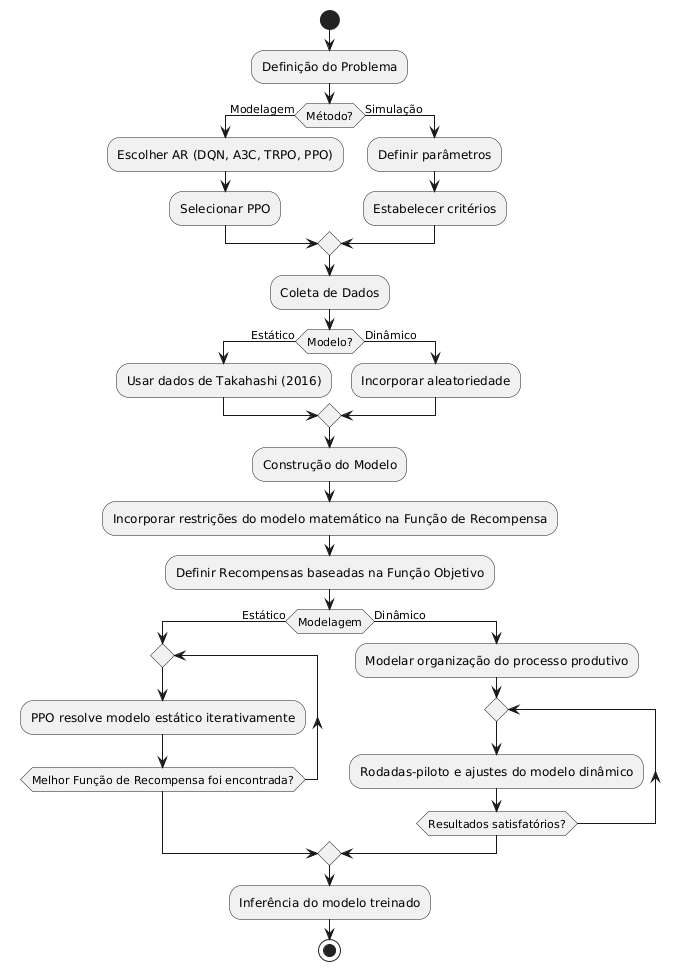
\includegraphics[width=0.9\textwidth]{figures/Metodo de pesquisa.png}
\end{figure}

\chapter{MODELO MATEMÁTICO}

A fim de validar o método alternativo de aprimoramento a ser proposto, emprega-se o modelo matemático desenvolvido por \citeonline{takahashi_2016} como parâmetro de comparação. Esse modelo fornece soluções ótimas ao problema e será usado como \textit{benchmark} para avaliar a eficácia da abordagem alternativa proposta.

Entre as diversas formulações apresentadas no referido trabalho, opta-se especificamente por aquela dedicada a auxiliar a decisão na escolha de fardos em estoque com base em características não categorizáveis. Essa seleção justifica-se porque tais características exercem impacto direto na qualidade final do produto e exigem maior precisão no momento da mistura.

Em seguida, detalham-se os tipos de características do algodão classificados como não categorizáveis. Cada uma dessas propriedades deve ser considerada e respeitada em sua média na mistura, de modo que o resultado atenda às especificações pré-estabelecidas pela empresa.

O objetivo consiste em fazer com que a média de cada característica atinja um valor-alvo específico, de forma a minimizar a diferença entre as médias obtidas na mistura e o alvo, garantindo que o produto atenda aos padrões de qualidade definidos.

Considerando as características $+b$, $rd$ e $Micronaire$ a serem controladas, definem-se os seguintes elementos do modelo:

Parâmetros:

\begin{itemize}
    \item $+b_p$ = valor de $+b$ nos fardos da procedência $p$.
    \item $rd_p$ = valor de $rd$ nos fardos da procedência $p$.
    \item $m_p$ = valor de $m$ (\textit{Micronaire}) nos fardos da procedência $p$.
    \item $E_p$ = quantidade de fardos de procedência $p$ em estoque.
    \item $D_k$ = número total de fardos utilizados na mistura $k$.
    \item $Q_k$ = quantidade de repetições na mistura $k$.
    \item $(+b)$ = valor-alvo para a característica $+b$ na mistura.
    \item $(rd)$ = valor-alvo para a característica $rd$ na mistura.
    \item $(m)$ = valor-alvo para a característica $m$ (\textit{Micronaire}) na mistura.
    \item $\lambda^{+b}$ = peso de normalização da característica $+b$.
    \item $\lambda^{rd}$ = peso de normalização da característica $rd$.
    \item $\lambda^{m}$ = peso de normalização da característica $m$.
\end{itemize}

Variáveis de decisão:
\begin{itemize}
    \item $X_{pk}$ = quantidade de fardos de procedência $p$ utilizados na mistura $k$.
    \item $A_k$ = diferença absoluta entre a média de $+b$ na mistura $k$ e o valor-alvo.
    \item $B_k$ = diferença absoluta entre a média de $rd$ na mistura $k$ e o valor-alvo.
    \item $C_k$ = diferença absoluta entre a média de $m$ na mistura $k$ e o valor-alvo.
\end{itemize}

A seguir, apresentam-se as diferenças entre as médias de cada característica para uma mistura $k$. O termo dentro do valor absoluto é a subtração entre a média da nova mistura (primeiro termo) e o valor-alvo que se deseja atingir (segundo termo). 

\begin{equation}
\left| \frac{\sum_{p=1}^{P} (+b_p * X_{pk})}{D_k} - (+b) \right| = A_k 
\end{equation}

\begin{equation}
\left| \frac{\sum_{p=1}^{P} (rd_p * X_{pk})}{D_k} - (rd) \right| = B_k 
\end{equation}

\begin{equation}
\left| \frac{\sum_{p=1}^{P} (m_p * X_{pk})}{D_k} - (m) \right| = C_k 
\end{equation}

Como $A_k$, $B_k$ e $C_k$ são resultados de grandezas distintas, torna-se imprescindível ponderar cada diferença para evitar que uma característica sobreponha as outras na busca pela solução ótima. Para tanto, atribuem-se pesos de normalização, conforme segue:

\begin{itemize}
    \item $\lambda^{+b}$ = peso para normalizar a grandeza $+b$.
    \item $\lambda^{rd}$ = peso para normalizar a grandeza $rd$.
    \item $\lambda^{m}$ = peso para normalizar a grandeza $m$.
\end{itemize}

Para definição desses pesos, utiliza-se a média da característica observada nos fardos em estoque:

\begin{equation}
\lambda = \frac{1}{\text{média da característica nos fardos em estoque}} 
\end{equation}

A função objetivo minimiza as diferenças absolutas entre as médias das características $+b$, $rd$ e $m$ nas misturas e os valores-alvo, ponderadas pelos pesos normalizadores $\lambda$. É definida como:

\begin{equation}
\text{Minimizar } \sum_{k=1}^{K} \left( \lambda^{+b} \cdot A_k + \lambda^{rd} \cdot B_k + \lambda^{m} \cdot C_k \right) \cdot Q_k
\end{equation}


As diferenças absolutas das características $+b$, $rd$ e $m$ em relação aos valores-alvo são definidas pelas seguintes restrições:

\begin{equation}
A_k \geq \frac{\sum_{p=1}^{P} (+b_p \cdot X_{pk})}{D_k} - (+b), \quad \forall k
\end{equation}

\begin{equation}
A_k \geq (+b) - \frac{\sum_{p=1}^{P} (+b_p \cdot X_{pk})}{D_k}, \quad \forall k
\end{equation}

\begin{equation}
A_k \geq 0, \quad \forall k
\end{equation}

\begin{equation}
B_k \geq \frac{\sum_{p=1}^{P} (rd_p \cdot X_{pk})}{D_k} - (rd), \quad \forall k
\end{equation}

\begin{equation}
B_k \geq (rd) - \frac{\sum_{p=1}^{P} (rd_p \cdot X_{pk})}{D_k}, \quad \forall k
\end{equation}

\begin{equation}
B_k \geq 0, \quad \forall k
\end{equation}

\begin{equation}
C_k \geq \frac{\sum_{p=1}^{P} (m_p \cdot X_{pk})}{D_k} - (m), \quad \forall k
\end{equation}

\begin{equation}
C_k \geq (m) - \frac{\sum_{p=1}^{P} (m_p \cdot X_{pk})}{D_k}, \quad \forall k
\end{equation}

\begin{equation}
C_k \geq 0, \quad \forall k
\end{equation}

As restrições de demanda e estoque garantem que o total de fardos utilizados satisfaça a demanda e respeite os limites do estoque disponível:

\begin{equation}
\sum_{p=1}^{P} X_{pk} = D_k, \quad \forall k
\end{equation}

\begin{equation}
\sum_{k=1}^{K} (X_{pk} \cdot Q_k) \leq E_p, \quad \forall p
\end{equation}

Por fim, o domínio das variáveis define que $X_{pk}$, a quantidade de fardos de procedência $p$ na mistura $k$, seja um número inteiro não negativo:

\begin{equation}
X_{pk} \in \mathbb{Z}^+, \quad \forall p, \forall k
\end{equation}

\section{ATUALIZAÇÃO DO ESTOQUE}

No modelo matemático empregado, a otimização busca determinar a mistura ideal com base exclusivamente no estoque disponível no momento da resolução, sem considerar a evolução dos estoques ou decisões em períodos futuros.

Em cada iteração, o modelo resolve o problema de mistura, calculando as quantidades de fardos \(X_{pk}\) a serem utilizados. Após a obtenção da solução, os estoques são ajustados, subtraindo-se os fardos consumidos, e o processo é repetido até que não haja mais uma solução factível, com os resultados sendo registrados a cada etapa.

\section{REPETIÇÃO DAS MISTURAS}

O parâmetro \( Q_k \) define o número de vezes que uma determinada mistura \( k \) deve ser repetida. Alterar o valor de \( Q_k \) possibilita diferentes estratégias de otimização. Por exemplo, ao definir \( Q_k > 1 \), impõe-se uma repetição fixa para cada mistura, o que pode ser útil em cenários onde se busca uniformidade na produção ou quando há restrições logísticas que favoreçam um número constante de misturas. Por outro lado, valores menores de \( Q_k \), como \( Q_k = 1 \), flexibilizam a abordagem, permitindo maior variação nas combinações e adaptando as misturas conforme a disponibilidade de estoque e as condições de qualidade exigidas.

Além disso, controlar \( Q_k \) pode impactar diretamente na estabilidade das características médias ao longo do processo produtivo. Um \( Q_k \) maior tende a gerar lotes mais homogêneos ao custo de reduzir a diversidade de misturas. Já \( Q_k \) menores promovem maior variação, o que pode ser vantajoso em situações onde a prioridade é atender à demanda com máxima eficiência no uso dos estoques disponíveis.

Na solução alternativa proposta, bem como na configuração do modelo matemático, opta-se por definir \( Q_k = 1 \). Dessa forma, não se estabelece um número fixo de repetições para as misturas, permitindo que estas possam se repetir, mas sem que isso seja uma restrição no modelo.

\section{ESTOQUE INICIAL E VALOR-ALVO}

A Tabela \ref{tab:valores_lambda} apresenta a média aritmética para todas as procedências em estoque, para cada característica estudada (\textit{rd}, \textit{\(+b\)} e \textit{Micronaire}), o valor-alvo adotado (definido internamente pela empresa estudada, no trabalho de \citeonline{takahashi_2016}) e os respectivos pesos normalizadores, obtidos a partir do inverso das médias de cada uma das características, a fim de remover as diferentes ordens de grandeza para a formulação da função objetivo. 

\begin{table}[htp]
    \centering
    \caption{Cálculo das médias, valores-alvo e pesos normalizadores (\(\lambda\)).}
    \begin{tabular}{c c c c}
         Característica & Média no Estoque & Valor Alvo & \(\lambda\) \\
         \hline
         \(rd\)         & 73,90  & 74,35  & 0,0135318 \\ 
         \(+b\)         & 9,98   & 9,34   & 0,1001669 \\ 
         \(Micronaire\) & 3,88   & 3,90   & 0,2535018 \\ 
         \hline
    \end{tabular}
    \label{tab:valores_lambda}
\end{table}

\chapter{MODELO DE APRENDIZADO POR REFORÇO}

Diferentemente da programação matemática, o AR resolve problemas explorando o ambiente por tentativa e erro, sem restrições explícitas. O comportamento do agente é guiado por uma função de recompensa, que avalia suas ações com base em condições pré-estabelecidas e atribui um \textit{feedback} correspondente. As restrições do problema são implicitamente representadas pela função de recompensa: ações que levam a soluções infactíveis recebem \textit{feedbacks} negativos, enquanto as factíveis são positivamente recompensadas, proporcionalmente ao objetivo do problema.

A função objetivo de um modelo matemático pode ser representada na função de recompensa do AR, retornando valores que reflitam o objetivo do problema. Embora o AR não exija estritamente que esses valores sejam contínuos, ele se beneficia significativamente dessa característica. Por exemplo, em um problema de otimização de custos, uma função de recompensa que atribui valores proporcionais ao custo total da solução — quanto menor o custo, maior a recompensa — facilita que o agente ajuste suas ações progressivamente, identificando políticas mais eficientes ao longo do tempo.

Se a recompensa for discretizada, como ao atribuir ``1'' para ações viáveis e ``0'' para inviáveis, o agente ainda pode aprender, mas sua capacidade de distinguir soluções boas de ótimas será reduzida, potencialmente retardando a convergência para uma solução de alta qualidade. 

\section{DISCRETIZAÇÃO}

Por ser um método iterativo de melhoria que utiliza a simulação de eventos discretos como ambiente de aprendizado, a demanda computacional é significativa. Para isso, testes computacionais foram realizados para encontrar o valor mínimo de discretização viável. 

O problema, em sua forma integral, considera 150 fardos em cada mistura, resultando em 150 variáveis de decisão no campo das ações e, para cada uma delas, 60 valores de procedências possíveis. Para reduzir a demanda computacional, foram testadas discretizações reduzindo a quantidade de fardos por mistura, com valores de 75 fardos (\(D=2\)), 50 fardos (\(D=3\)), 30 fardos (\(D=5\)), 25 fardos (\(D=6\)) e 15 fardos (\(D=10\)). Para preservar a natureza do problema, a quantidade de itens em estoque para cada procedência também foi proporcionalmente reduzida, dividindo-a pelo valor de \(D\).


\section{ABORDAGEM ESTÁTICA E DETERMINÍSTICA}

Para validar diretamente as soluções encontradas pelo AR em relação ao modelo matemático, o problema é modelado com premissas estáticas e determinísticas.

Nesse cenário, o estoque inicial é fixo, sem renovação, e todas as variáveis do processo são consideradas conhecidas e imutáveis, eliminando incertezas. Os mesmos dados utilizados no modelo matemático são reaproveitados, incluindo os valores de estoque das procedências, suas respectivas características e os valores-alvo previamente definidos.

Dito isso, o problema é tratado, inicialmente, da seguinte forma:
\begin{itemize}
    \item Ações: escolha das procedências dos fardos a serem misturados (150 no total) no período $t$.
    \item Observações: registro dos fardos escolhidos no período anterior ($t-1$).
    \item Recompensa: valor inversamente proporcional à função objetivo, variando entre 0 e 1.
\end{itemize}

A recompensa é definida como:

\begin{equation}
    R = \frac{1}{1 + \text{FO}}
\end{equation}

$\text{FO}$ representa o valor da função objetivo, calculado com base na diferença do valor das propriedades $rd$, $+b$ e $Micronaire$ em relação aos valores-alvo. Quando $\text{FO}$ é igual a zero, as propriedades atingem exatamente os valores-alvo, resultando no valor máximo de $R = 1$. À medida que $\text{FO}$ aumenta, indicando desvios crescentes em relação aos alvos, o valor de $R$ tende a zero, desincentivando soluções distantes dos objetivos estabelecidos.

Do ponto de vista das restrições do problema, no AR, não se pode impô-las diretamente ao agente, como ocorre em modelos matemáticos. Ao contrário disso, a função de recompensa e o ambiente de aprendizado devem ser construídos para representar as limitações e requisitos do problema real.

Em um modelo matemático, as restrições são definidas de forma exata: soluções que violam essas restrições são automaticamente descartadas pelo otimizador, garantindo que apenas resultados factíveis sejam considerados. Por exemplo, se uma restrição determina que a soma das variáveis deve ser menor ou igual a um limite específico, qualquer solução que exceda esse limite será rejeitada sem uma avaliação gradual.

No AR, adotar essa abordagem direta é contraproducente para o aprendizado do agente. Se todas as violações forem tratadas como igualmente infactíveis, atribuindo-se um mesmo valor de punição a todas elas, o agente não consegue distinguir entre violações graves e leves. Isso dificulta sua capacidade de ajustar as ações para se aproximar de soluções factíveis.

Para contornar esse problema, a função de recompensa deve incluir incentivos graduais que penalizem o agente proporcionalmente à gravidade das violações das restrições.

\subsection{RL I: FUNÇÃO DE RECOMPENSA PADRÃO}

Nesta abordagem inicial, a recompensa é definida como inversamente proporcional à função objetivo (\( \text{FO} \)), que mede os desvios das características \(rd\), \(+b\), e \(Micronaire\) em relação aos valores-alvo. Adicionalmente, uma penalização fixa de \(-1\) é aplicada quando a mistura contém menos fardos do que o esperado (\(D_k < \text{Esperado}\)). A recompensa é representada por:

\begin{equation}
R = \frac{1}{1 + \text{FO}} - \delta(D_k < \text{Esperado})
\end{equation}

O termo \(\delta(D_k < \text{Esperado})\) é definido como:
\[
\delta(D_k < \text{Esperado}) =
\begin{cases} 
1, & \text{se } D_k < \text{Esperado}, \\
0, & \text{caso contrário.}
\end{cases}
\]

A natureza binária da penalização reflete diretamente a implementação no código, onde uma instrução condicional (\texttt{if}) avalia se a quantidade de fardos na mistura está abaixo do valor esperado. 

\subsection{RL II: PUNIÇÃO PROPORCIONAL ÀS PROPRIEDADES DISTANTES DO ALVO E OBSERVAÇÃO DO ESTOQUE}

Nesta versão, além das características do RL I, é adicionada uma penalização proporcional à distância percentual de cada propriedade (\(+b\), \(rd\) e \(Micronaire\)) em relação aos valores-alvo. Adicionalmente, o agente recebe como observação a quantidade de fardos restantes no estoque para cada procedência, permitindo melhores ajustes considerando o horizonte de planejamento, de forma que irá associar determinadas ações às condições do estoque após o treinamento. A recompensa é reformulada como:

\begin{equation}
R = \frac{1}{1 + \text{FO}} - \delta(D_k < \text{Esperado}) - \sum_{i \in \{rd, +b, m\}} \Delta_i
\end{equation}

Onde:
\begin{equation}
\Delta_i =
\begin{cases} 
\frac{x}{100}, & \text{se } \left| \text{Propriedade}_{\text{atual}} - \text{Propriedade}_{\text{alvo}} \right| > x\%, \\
0, & \text{caso contrário.}
\end{cases}
\end{equation}

Essa modificação incentiva o agente a minimizar gradativamente os desvios das propriedades-alvo e a respeitar os limites de quantidade de fardos esperados, enquanto a observação do estoque possibilita decisões mais informadas. Ademais, ainda é possível definir qual o melhor valor de \textit{x} para o aprendizado do agente.

\subsection{RL III: AUMENTO DA PUNIÇÃO PARA SOLUÇÕES INFACTÍVEIS}

Com base no RL II, esta versão aumenta a penalização para misturas que contenham menos fardos do que o esperado, passando de \(-1\) para \(-2\). Esse ajuste reforça a importância de atender à restrição de quantidade total de fardos, diferenciando-a das penalizações proporcionais associadas aos desvios das características \(rd\), \(+b\) e \(Micronaire\). A recompensa é reformulada como:

\begin{equation}
R = \frac{1}{1 + \text{FO}} - \delta(D_k < \text{Esperado}) \cdot 2 - \sum_{i \in \{rd, +b, m\}} \Delta_i
\end{equation}

A principal modificação em relação ao RL II é o aumento da penalização fixa para soluções infactíveis relacionadas à quantidade total de fardos. Essa distinção atribui maior prioridade a essa restrição, indicando que, no contexto do problema, soluções com menos fardos que o esperado são significativamente mais prejudiciais ao sistema do que desvios moderados nas características-alvo. 

\subsection{RL IV: INCLUSÃO DE DOIS PERÍODOS DE DEFASAGEM NAS OBSERVAÇÕES}

Neste modelo, o histórico de decisões do agente é expandido para incluir informações do período anterior (\(t-2\)), além do período mais recente (\(t-1\)). Isso permite que o agente aprenda padrões mais complexos e ajuste ações com base em decisões passadas. 

\subsection{RL V: AUMENTO EXTREMO DAS PUNIÇÕES EM SOLUÇÕES INFACTÍVEIS}

Nesta versão, a penalização fixa para misturas com menos fardos do que o esperado é elevada de \(-2\) para \(-33\). Esse valor é suficientemente alto para que soluções infactíveis com relação à quantidade de fardos no misturador neutralizem todas as recompensas acumuladas em outras soluções factíveis. O objetivo é forçar o agente a evitar completamente soluções que violem esta restrição crítica. A recompensa é formulada como:

\begin{equation}
R = \frac{1}{1 + \text{FO}} - \delta(D_k < \text{Esperado}) \cdot 33 - \sum_{i \in \{rd, +b, m\}} \Delta_i
\end{equation}

\subsection{RL VI: RECOMPENSA EXTRA PARA FO = 0}

Nesta versão, um incentivo adicional é introduzido para reforçar soluções que atingem exatamente os valores-alvo das propriedades (\(rd\), \(+b\) e \(Micronaire\)), ou seja, quando \(\text{FO} = 0\). Este incremento adiciona uma recompensa fixa de \(+2\), criando um estímulo significativo para que o agente priorize a busca por soluções ótimas nas misturas iniciais. A recompensa é formulada como:

\begin{equation}
R = \frac{1}{1 + \text{FO}} + \beta(\text{FO} = 0) \cdot 2 - \delta(D_k < \text{Esperado}) \cdot 2 - \sum_{i \in \{rd, +b, m\}} \Delta_i
\end{equation}

O incentivo adicional para \(\text{FO} = 0\) diferencia soluções ótimas de outras factíveis, incentivando o agente a maximizar a qualidade das misturas.

\subsection{RL VII: OBSERVAÇÃO BINÁRIA DO ESTOQUE}

Nesta versão, a observação do ambiente foi ajustada para incluir uma variável binária associada a cada procedência, indicando a presença (\(1\)) ou ausência (\(0\)) de fardos em estoque. Esse ajuste foi implementado para comparar o desempenho do modelo ao utilizar essa representação binária com a abordagem anterior, que fornecia as quantidades de fardos restantes em valores inteiros.

A estrutura da recompensa segue a mesma do RL VI, com o incentivo para soluções ótimas e penalizações por desvios e soluções infactíveis.


\subsection{TESTES COM O HIPERPARÂMETRO \textit{clip\_range}}

No PPO, o hiperparâmetro \textit{clip\_range}, correlato à técnica de \textit{clipping}, influencia diretamente a estabilidade e a eficiência do treinamento. Este parâmetro controla o tamanho máximo da atualização permitida na política do agente, evitando alterações que poderiam levar a instabilidades ou perda de desempenho durante o aprendizado \cite{schulman_proximal_2017}.

O \textit{clip\_range} define o intervalo permitido para o valor da razão entre as probabilidades da política atual e da política anterior para as ações realizadas. Se essa razão ultrapassar o limite definido (\(1 \pm \epsilon\), onde \(\epsilon\) é o valor de \textit{clip\_range}), a atualização é truncada para evitar mudanças excessivas.

Para avaliar o impacto do \textit{clip\_range} no desempenho do agente, testes foram realizados utilizando o modelo RL III com os seguintes valores: \(0,1\), \(0,2\) (padrão), \(0,5\) e \(1,0\). 

\section{ABORDAGEM DINÂMICA E ESTOCÁSTICA}

O estoque inicial, anteriormente conhecido, passa a ser construído de forma aleatória. As quantidades totais de fardos em estoque permanecem inalteradas; no entanto, as proporções de cada procedência são definidas por meio de um sorteio. Além disso, é estabelecido um tempo de processamento para o processo de mistura, que consome o estoque disponível, bem como um intervalo entre cada reposição desse estoque. Ambas as taxas são fictícias, sendo modeladas por uma distribuição \textit{Normal} de probabilidade, com o mesmo desvio padrão e uma média ajustada de modo a manter o equilíbrio do sistema ao longo do tempo, considerando misturas com quantidades factíveis de fardos.

O equilíbrio do sistema é definido por:

\begin{itemize}
    \item \( C \) – número fixo de fardos consumidos por mistura;
    \item \( T_m \) – tempo médio de processamento de uma mistura;
    \item \( T_r \) – tempo médio entre reposições do estoque;
    \item \( R \) – número de fardos repostos por chegada.
\end{itemize}

Embora \( R \) seja sorteado a cada reposição, a longo prazo, sua média tende a uma expectativa estatística baseada na distribuição do estoque inicial. Assim, o equilíbrio é expresso por:

\begin{equation}
    \frac{C}{T_m} = \frac{\mathbb{E}[R]}{T_r}
\end{equation}

Isolando \( T_r \), obtém-se:

\begin{equation}
    T_r = \frac{\mathbb{E}[R]}{C} \cdot T_m
\end{equation}

Logo, para manter o sistema balanceado, o tempo entre reposições \( T_r \) deve ser ajustado proporcionalmente ao tempo de mistura \( T_m \), levando em conta a expectativa da quantidade de fardos repostos.

Assumindo que \( R \) segue uma distribuição normal \( \mathcal{N}(\mu_R, \sigma^2) \), a relação esperada entre os tempos é:

\begin{equation}
    \mu_{T_r} = \frac{\mu_R}{C} \cdot \mu_{T_m}
\end{equation}

Onde \( \mu_{T_r} \) representa a média do tempo entre reposições e \( \mu_{T_m} \) a média do tempo de mistura.

A chegada de novos fardos, por sua vez, utiliza a distribuição do estoque inicial como referência para definir as probabilidades de seleção das procedências. No modelo estático e determinístico, o estoque inicial era previamente conhecido, contendo 60 procedências, cada uma com quantidades distintas. No entanto, no modelo atual, a chegada de fardos é aleatória, sorteando-se \( X \) procedências e suas respectivas quantidades a cada chegada.

A quantidade de procedências \( X \) sorteadas em cada chegada é definida de modo a respeitar o equilíbrio do sistema a longo prazo, conforme estabelecido pela relação entre o tempo de processamento das misturas \( T_m \) e o tempo entre reposições \( T_r \).

As propriedades dos fardos escolhidos, como \textit{rd}, \textit{+b} e \textit{Micronaire}, são ajustadas de forma aleatória dentro de uma faixa de variação de \(-10\%\) a \(+10\%\) em relação aos valores originais.

\begin{equation}
    P = P_0 + U(-0.1 P_0, 0.1 P_0)
\end{equation}

Onde:

\begin{itemize}
    \item \( P \) – valor ajustado da propriedade do fardo;
    \item \( P_0 \) – valor original da propriedade;
    \item \( U(-0.1 P_0, 0.1 P_0) \) – variação aleatória uniforme de até \( \pm 10\% \) do valor original.
\end{itemize}


\section{MODELO DE SIMULAÇÃO}

A fim de integrar todas as premissas propostas para o ambiente de aprendizado, bem como outras ferramentas de conectividade de dados, o simulador de eventos discretos e gêmeo digital \textit{FlexSim} é utilizado.

Por se tratar de um \textit{software} com permissividade de representação gráfica tridimensional do processo, é possível incorporar customizações visuais que aproximam a simulação do contexto real, facilitando a compreensão das soluções propostas a posteriori.

Nesta seção, será tratado apenas do modelo de simulação referente à segunda abordagem discutida, que incorpora a aleatoriedade ao processo. 

Na Figura \ref{figure:estoqueemisturador} temos a representação de um fardo de algodão e de parte do processo de fiação têxtil, considerando 34 baias de estoque (\textit{Box}) e um misturador.

\begin{figure}[hbt]
\centering
  \caption{Representação 3D do processo e do fardo de algodão.}
  \label{figure:estoqueemisturador}
  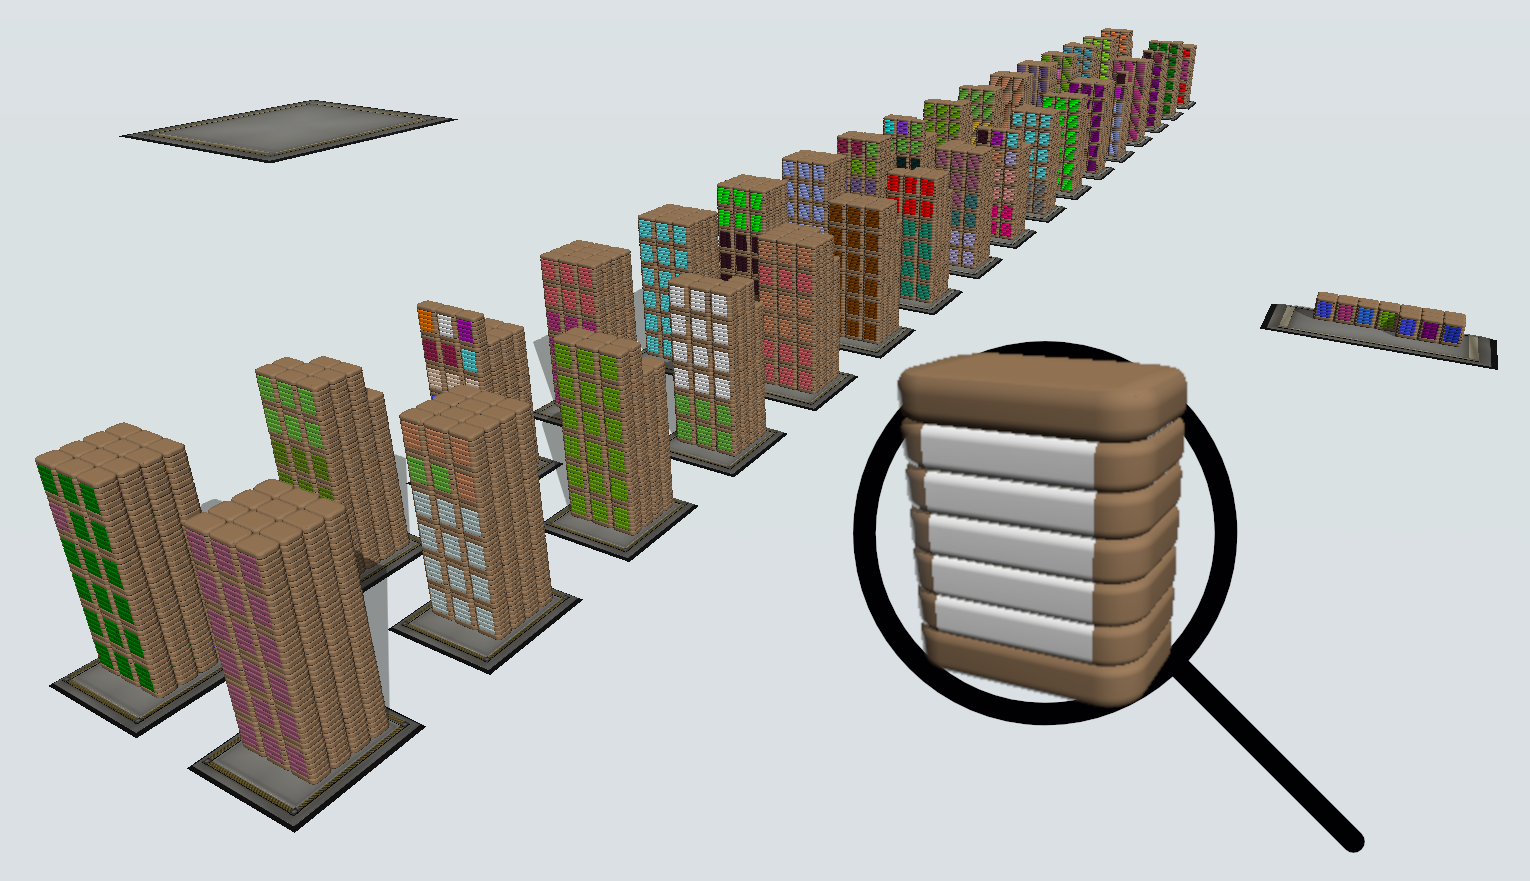
\includegraphics[width=1\textwidth]{figures/simulação.png}
\end{figure}

O simulador se divide em duas partes distintas: \textit{Model 3D} e \textit{Process Flow}. Ambas seguem os princípios da Programação Orientada a Objetos \cite{poo_1982}, sendo a primeira voltada a objetos físicos tridimensionalmente representados e conectados por um fluxo, enquanto a segunda é abstrata, organizada por blocos e complementar à primeira.

Dado que o \textit{Process Flow} permite maior liberdade para a modelagem da simulação, o \textit{Model 3D} se restringe apenas para às lógicas de direcionamento do fluxo visto na Figura \ref{figure:fluxoUML}.

\begin{figure}[hbt]
\centering
  \caption{Fluxo dos fardos no processo.}
  \label{figure:fluxoUML}
  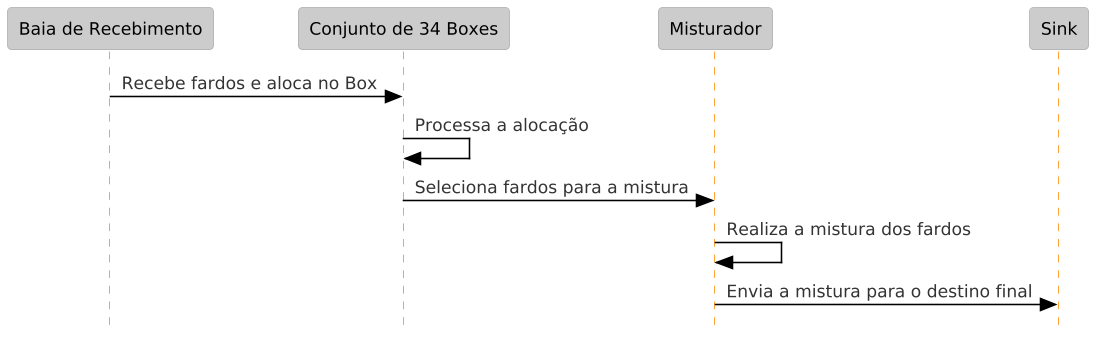
\includegraphics[width=1\textwidth]{figures/fluxoUML.png}
\end{figure}

Para dar início ao fluxo, os fardos são gerados a partir do \textit{Process Flow}, onde lógicas de sorteio e atribuição de propriedades são ativadas por um \textit{token} circulante. O fluxo é estruturado em duas partes principais: a primeira reproduz o estoque inicial da abordagem estática e determinística, além de gerar novas chegadas ao longo do tempo, realizando o sorteio dos fardos e de suas respectivas propriedades; a segunda gerencia as portas de entrada e saída dos \textit{boxes} e do misturador, garantindo a sincronização do fluxo sequencial dos estados do sistema e sua integração com os gatilhos do AR. Na Figura \ref{figure:ProcessFlow}, isso pode ser observado.

\begin{figure}[hbt]
\centering
  \caption{\textit{Process Flow} para gerenciamento do fluxo.}
  \label{figure:ProcessFlow}
  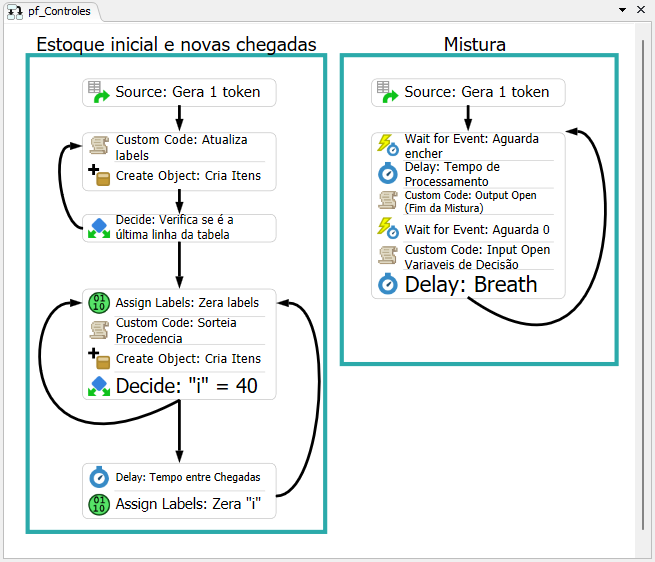
\includegraphics[width=1\textwidth]{figures/ProcessFlow.png}
\end{figure}

Assim que os fardos são gerados como objetos na simulação, eles são alocados nas baias de armazenamento de acordo com uma lógica que busca racionalizar a organização dos \textit{boxes} de estoque e seus respectivos fardos. 

Inicialmente, verifica-se se existe uma baia que já contenha itens da mesma procedência do novo item. Caso exista e a quantidade de itens nessa baia esteja dentro do limite permitido, o item é alocado nela. Caso contrário, busca-se uma baia vazia para armazená-lo. Se não houver baias vazias disponíveis, o item é direcionado para a baia que possui a menor quantidade de itens, garantindo uma distribuição equilibrada da carga de armazenamento. O Algoritmo \ref{alg:alocacao_balanceada} evidencia essas relações.

\begin{algorithm}[H]
\caption{Pseudocódigo da lógica de alocação de fardos nos \textit{boxes}}
\label{alg:alocacao_balanceada}
\KwEntrada{Item \(it\), Lista de \textit{boxes} \(bx\)}
\KwSaida{Índice da baia selecionada \(selBx\)}

\(nBx \gets \text{tamanho}(bx)\)\;
\(selBx \gets 0\)\;
\(limite \gets 2 \times nBx\)\;
\(proc \gets it.proc\)\;
\(minQtd \gets \infty\)\;

\Para{\(i \gets 1\) \textbf{até} \(nBx\) }{
    \(b \gets bx[i]\)\;
    \Se{\(possuiProc(b, proc)\) \textbf{e} \(\text{tamanho}(b) < limite\)}{
        \(selBx \gets i\)\;
        \Retorne{\(selBx\)}\;
    }
}
\Para{\(i \gets 1\) \textbf{até} \(nBx\) }{
    \Se{\(\text{tamanho}(bx[i]) = 0\)}{
        \(selBx \gets i\)\;
        \Retorne{\(selBx\)}\;
    }
}
\Para{\(i \gets 1\) \textbf{até} \(nBx\) }{
    \Se{\(\text{tamanho}(bx[i]) < minQtd\)}{
        \(minQtd \gets \text{tamanho}(bx[i])\)\;
        \(selBx \gets i\)\;
        \Retorne{\(selBx\)}\;
    }
}

\end{algorithm}

O algoritmo recebe um item \(it\) e uma lista de baias \(bx\), retornando o índice do \textit{box} selecionado \(selBx\). Inicialmente, são definidas as seguintes variáveis:
\begin{itemize}
    \item \(nBx\): número total de \textit{boxes} contidos na lista \(bx\);
    \item \(selBx\): inicialmente definido como 0, indicando que nenhum box foi escolhido;
    \item \(limite\): calculado como o dobro do número total de \textit{boxes}, estabelecendo o teto de ocupação aceitável para um \textit{box};
    \item \(proc\): procedência do item \(it\);
    \item \(minQtd\): inicializado com \(\infty\), utilizado para identificar o \textit{box} com a menor quantidade de itens.
\end{itemize}

Em seguida, o algoritmo utiliza três critérios para selecionar a baia:
\begin{itemize}
    \item Critério 1 – Alocação por procedência:
    O algoritmo percorre a lista de \textit{boxes} e, para cada \textit{box} \(b\), verifica se ela já contém itens com a mesma procedência do item (através da função \(possuiProc(b, proc)\)) e se a quantidade de itens no \textit{box}, obtida por \(\text{tamanho}(b)\), é inferior ao limite estabelecido. Se ambas as condições forem satisfeitas, o \textit{box} é imediatamente selecionado e seu índice é retornado. 

    \item Critério 2 – Busca por \textit{box} vazio: 
    Se nenhum \textit{box} atender ao Critério 1, o algoritmo procura por um \textit{box} que esteja completamente vazio, isto é, para o qual \(\text{tamanho}(bx[i]) = 0\). A escolha de um \textit{box} vazio permite iniciar a alocação sem interferência de itens previamente alocados.

    \item Critério 3 – Seleção pela menor ocupação:  
    Caso os dois primeiros critérios não resultem na seleção de um \textit{box}, o algoritmo percorre novamente todos os \textit{boxes} para identificar aquele com a menor quantidade de itens. Durante essa etapa, a variável \(minQtd\) é atualizada e o \textit{box} com a menor carga é selecionado.
\end{itemize}

Por fim, o algoritmo retorna o índice da baia selecionada (\(selBx\)), determinando assim onde o item \(it\) deverá ser alocado. As funções \(tamanho(bx[i])\) e \(possuiProc(b, proc)\) são responsáveis, respectivamente, por retornar a quantidade de itens presentes em uma baia e por verificar se a procedência \(proc\) já se encontra na baia \(b\). 

\chapter{SISTEMA DE INFORMAÇÕES GERENCIAIS}

O sistema de informações gerenciais desempenha um papel essencial neste protocolo, pois, após o treinamento do agente por meio da simulação para tomar decisões informadas, busca-se a incorporação de dados reais do sistema. Nesse estágio, a aleatoriedade inerente à simulação é substituída pelo comissionamento virtual, permitindo uma operação baseada em informações concretas e representativas do ambiente real.

Como visto na Figura \ref{figure:SIG}, o SIG se relaciona com o protocolo como uma interface entre o ambiente físico e o digital, sendo por ele que se introduz e recebe as informações pertinentes ao auxílio na tomada de decisão. 

\begin{figure}[hbt]
\centering
  \caption{Diagrama Sequencial do protocolo proposto.}
  \label{figure:SIG}
  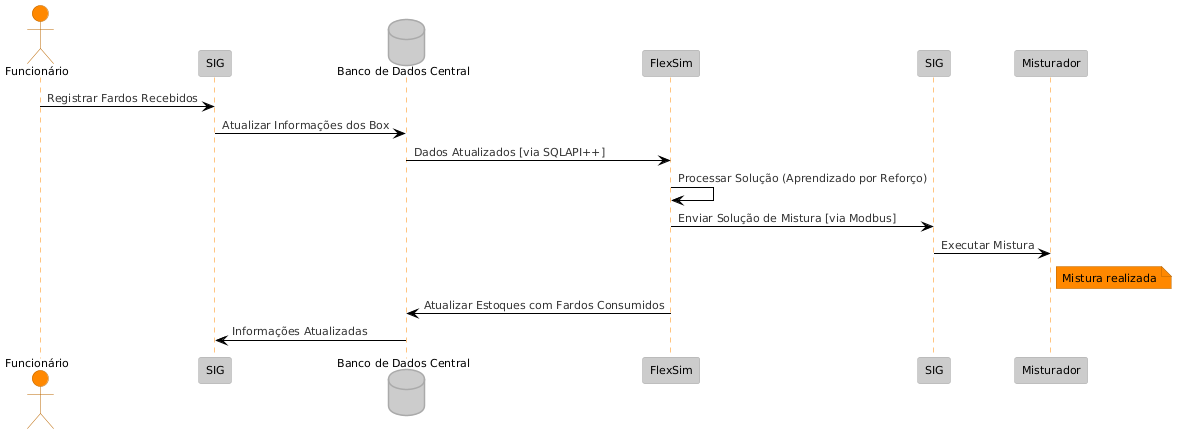
\includegraphics[width=1\textwidth]{figures/SIG.png}
\end{figure}

O sistema em \textit{Python} utiliza \textit{Flask}, \textit{SQLAlchemy} e um servidor \textit{MODBUS} para gerenciar procedências e estoques. Uma aplicação \textit{web} recebe inserções de dados, consolidando ocorrências de mesma procedência em uma estrutura de Banco de Dados \textit{PostgreSQL}. O servidor \textit{MODBUS}, executado em paralelo, disponibiliza um conjunto de registros para troca de informações, sendo o SIG desempenhando papel de cliente e o modelo de simulação o servidor. Os dados entram no \textit{FlexSim} a partir da sincronização do Banco de Dados \textit{PostgreSQL} com o modelo de simulação, por meio da \textit{SQLAPI++}. Conectado via protocolo \textit{MODBUS}, o \textit{FlexSim} obtém os valores necessários do sistema e retorna resultados de simulações ou execuções associadas às procedências.

Em paralelo, ocorre a execução do modelo treinado por AR, que ajusta a tomada de decisão a partir das interações com o ambiente simulado no \textit{FlexSim}, atualizado pelo ambiente real.


\section{ENTRADA DE DADOS}

Em um contexto operacional, no qual novos fardos chegam periodicamente e se deseja registrá-los de maneira simplificada, o colaborador responsável abriria a aplicação \textit{web} (Figura \ref{figure:TelaInput}) em qualquer dispositivo. Nessa aplicação, ele selecionaria as procedências e a quantidade de fardos a serem adicionados ao Banco de Dados. Ainda nessa interface, existe a opção de zerar todos os registros ou, por fins didáticos, replicar o perfil de estoque ilustrado na Tabela~\ref{tab:estoque_inicial}.

\begin{figure}[hbt]
\centering
  \caption{Tela de registro dos novos fardos.}
  \label{figure:TelaInput}
  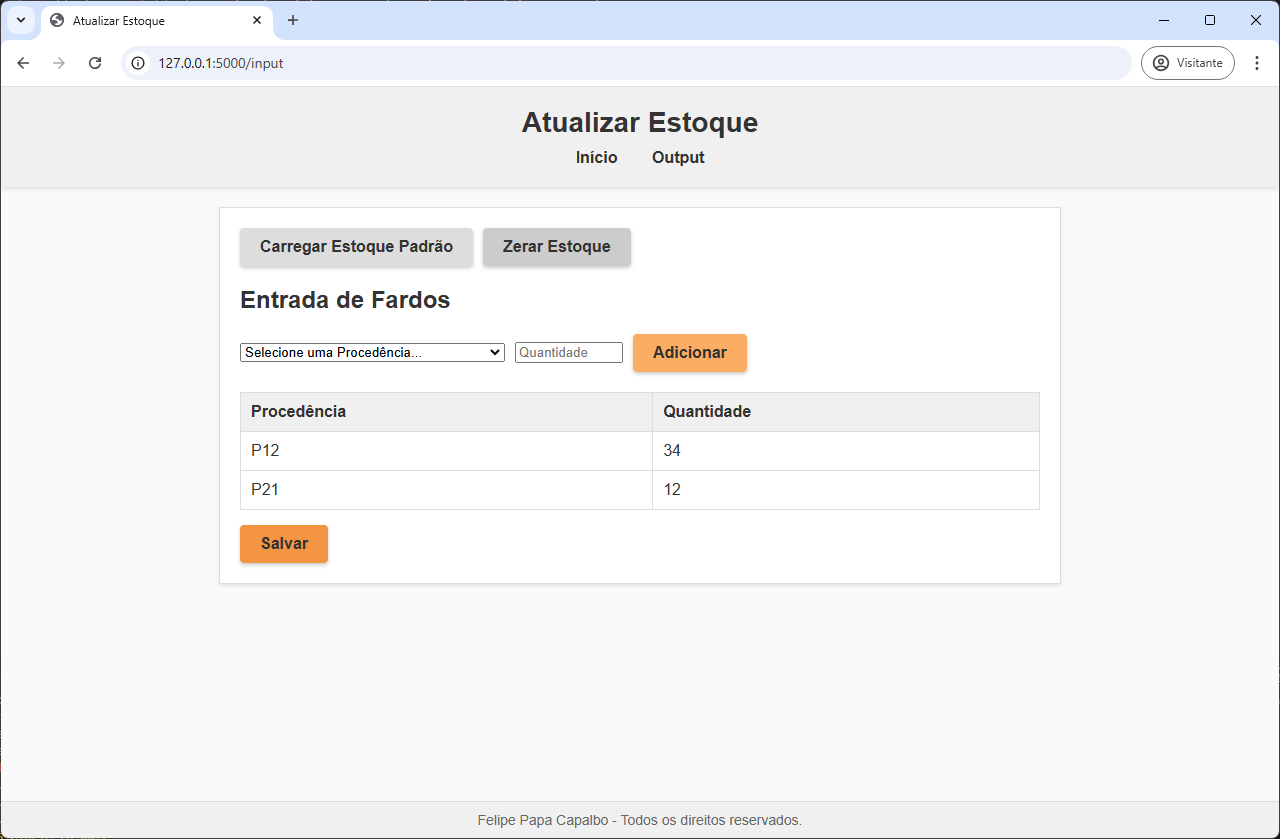
\includegraphics[width=1\textwidth]{figures/TelaInput.png}
\end{figure}

\section{BANCO DE DADOS RELACIONAL}

Para armazenar as informações de estoque e registrar quais fardos foram efetivamente utilizados em cada mistura, concebe-se um esquema de Banco de Dados relacional que se baseia em três tabelas interligadas. A tabela Estoque armazena as procedências e suas características (como quantidade, rd, +b, Micronaire), enquanto a tabela Mistura identifica cada evento ou processo de mistura que ocorre ao longo do tempo (com data, observações e demais atributos). Para relacionar os fardos escolhidos a cada mistura, define-se uma terceira tabela, MisturaEstoque, que funciona como uma ligação entre Mistura e Estoque, descrevendo quantos fardos de determinada procedência foram aplicados em cada mistura.

\begin{table}[htp]
    \centering
    \caption{Tabela Estoque, responsável por manter o estado atual de cada procedência.}
    \begin{tabular}{c c c c c}
         ID & estoque\_inicial & rd & +b & Micronaire \\ \hline
         PK, Inteiro & Inteiro, Default 0 & Float & Float & Float \\
    \end{tabular}
    \label{tab:tb_estoque}
\end{table}

\begin{table}[htp]
    \centering
    \caption{Tabela Mistura, que registra cada evento de mistura e suas informações gerais.}
    \begin{tabular}{c c c}
         ID & data\_hora & observacao \\ \hline
         PK, Inteiro & \textit{DateTime} & Texto, Opcional \\
    \end{tabular}
    \label{tab:tb_mistura}
\end{table}

\begin{table}[htp]
    \centering
    \caption{Tabela intermediária MisturaEstoque, que liga fardos (Estoque) às misturas (Mistura).}
    \begin{tabular}{c c c c}
         ID & mistura\_id & estoque\_id & quantidade \\ \hline
         PK, Inteiro & FK em Mistura.id & FK em Estoque.id & Inteiro \\
    \end{tabular}
    \label{tab:tb_mistura_estoque}
\end{table}

No \textit{script} em \textit{Python}, cada uma dessas tabelas é criada com o \textit{SQLAlchemy}. A Estoque guarda o estado atual de cada procedência (por exemplo, quantos fardos existem de uma dada origem, quais os valores de rd e +b). A Mistura representa o evento em si (data e observações). Por fim, a MisturaEstoque define quantos fardos de cada procedência foram empregados em determinada mistura, ligando Mistura (por meio de mistura\_id) à Estoque (via estoque\_id).

\section{SAÍDA DE DADOS}

As decisões produzidas pelo \textit{FlexSim} e obtidas por meio do protocolo \textit{MODBUS} são apresentadas em uma interface \textit{web}, por intermédio do mesmo \textit{script} em \textit{Python}. Na aplicação desenvolvida com \textit{Flask}, o servidor \textit{MODBUS} executa em paralelo, armazenando em registros específicos as informações retornadas pelo \textit{FlexSim}, como a procedência selecionada, eventuais ajustes na quantidade de fardos ou outra variável operacional. Esses registros são atualizados constantemente, de modo que a aplicação consiga refletir o estado atual do sistema.

A Figura~\ref{figure:TelaOutput} ilustra a tela de saída, onde as soluções provenientes do \textit{FlexSim} são exibidas. Cada atualização no \textit{FlexSim} escreve valores nos registradores \textit{MODBUS}, e o \textit{script} em \textit{Python} coleta esses valores e os organiza em elementos de visualização. Dessa forma, o colaborador consegue acompanhar a evolução das variáveis de interesse, além de verificar possíveis ajustes sugeridos pelo AR.

\begin{figure}[hbt]
\centering
  \caption{Tela de saída com informações recebidas do \textit{FlexSim} via \textit{MODBUS}.}  
  \label{figure:TelaOutput}
  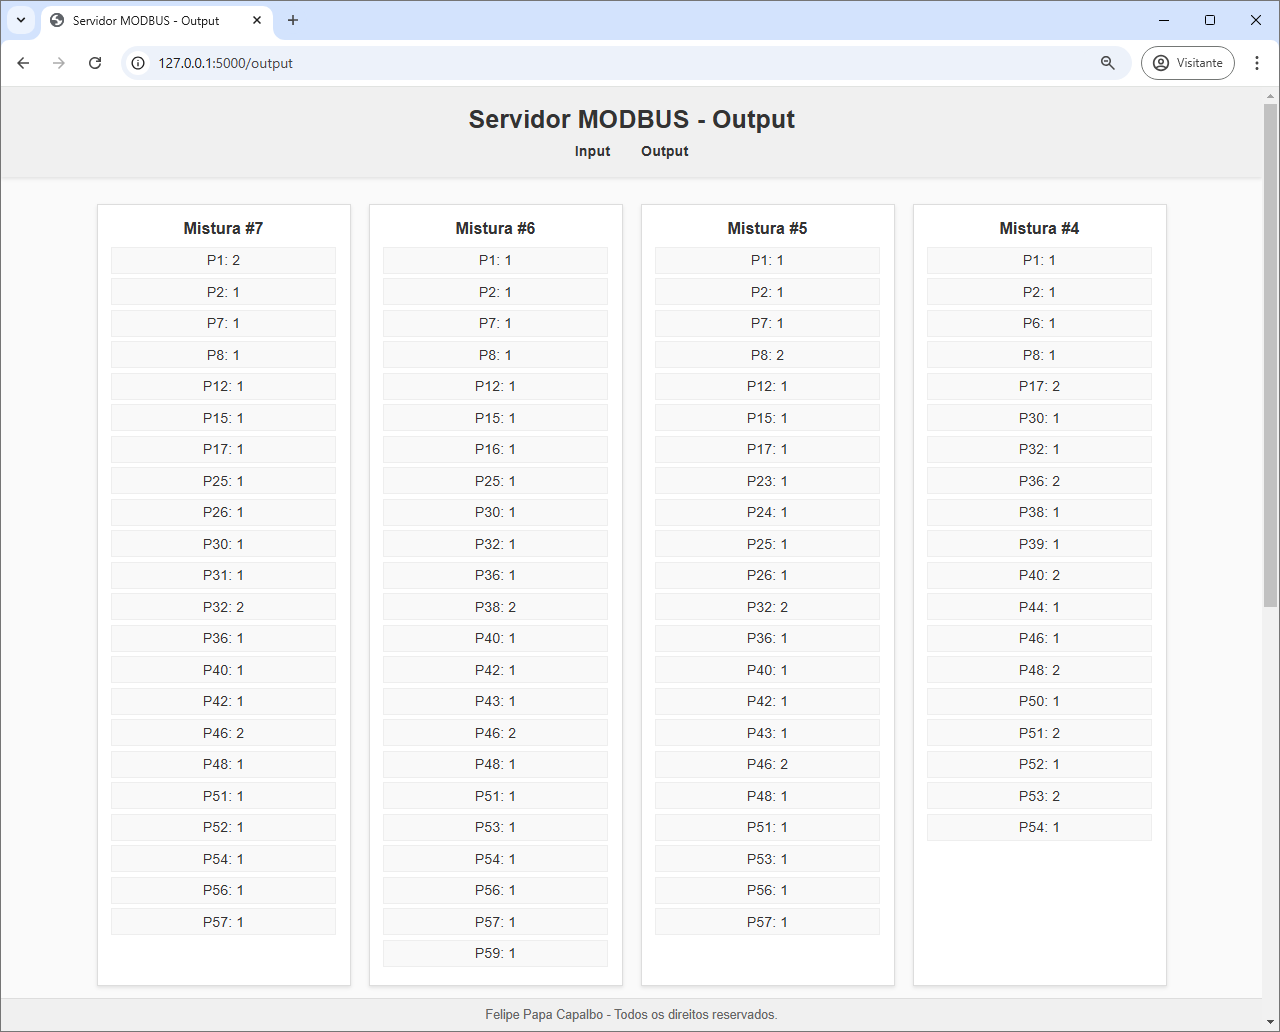
\includegraphics[width=1\textwidth]{figures/TelaOutput.png}
\end{figure}


De forma prática, foi construída uma rota \textit{/output}, na aplicação baseada em \textit{Flask}, que consiste em exibir os dados lidos do servidor \textit{MODBUS}. O \textit{script} utiliza o objeto \textit{DataBank} para armazenar valores nos registros \textit{holding}. Assim, cada nova decisão ou resultado de simulação, enviados pelo \textit{FlexSim}, é gravado na forma de inteiros ou pontos flutuantes. Uma \textit{thread} no \textit{Python} lê periodicamente esses valores, atualiza uma estrutura de dados e fornece as informações em formato \textit{JSON} para a interface \textit{web}. A página de saída, por sua vez, processa esse \textit{JSON} e exibe as decisões do sistema, permitindo a visualização consolidada das soluções advindas do \textit{FlexSim} e do algoritmo de AR.

\chapter{RESULTADOS}

No presente capítulo, serão apresentados os resultados computacionais do trabalho, podendo afirmar sua robustez, justificar as afirmações feitas e responder às questões de pesquisa previamente levantadas.

Para executar os modelos e \textit{scripts} citados, foi utilizado o CPU Intel(R) Core(TM) i5-11400F, com 6 núcleos físicos e 12 \textit{threads}, com \textit{clock} base de 2,60 GHz e máximo de 4,40 GHz (\textit{stock}); 16 GB de memória RAM DDR4 2666 MHz; e GPU Nvidia GeForce RTX 3060 TI 8 GB GDDR6.

\section{MODELO MATEMÁTICO}

Devido à alta demanda computacional dos modelos de AR, o problema teve de ser discretizado, ou seja, dividido em partes menores, preservando seus princípios comportamentais, mas com menos dados. Sob fins de comparação, o modelo matemático, sem discretização (MIP D1), que resolve o problema ao otimizar as misturas a partir de um estoque inicial fixo, de maneira iterativa e sem restrições para repetições de misturas, tem seus valores ótimos representados na Figura \ref{figure:MM}.

\begin{figure}[hbt]
\centering
  \caption{Misturas iterativas resolvidas pelo modelo matemático (MIP D1).}  
  \label{figure:MM}
  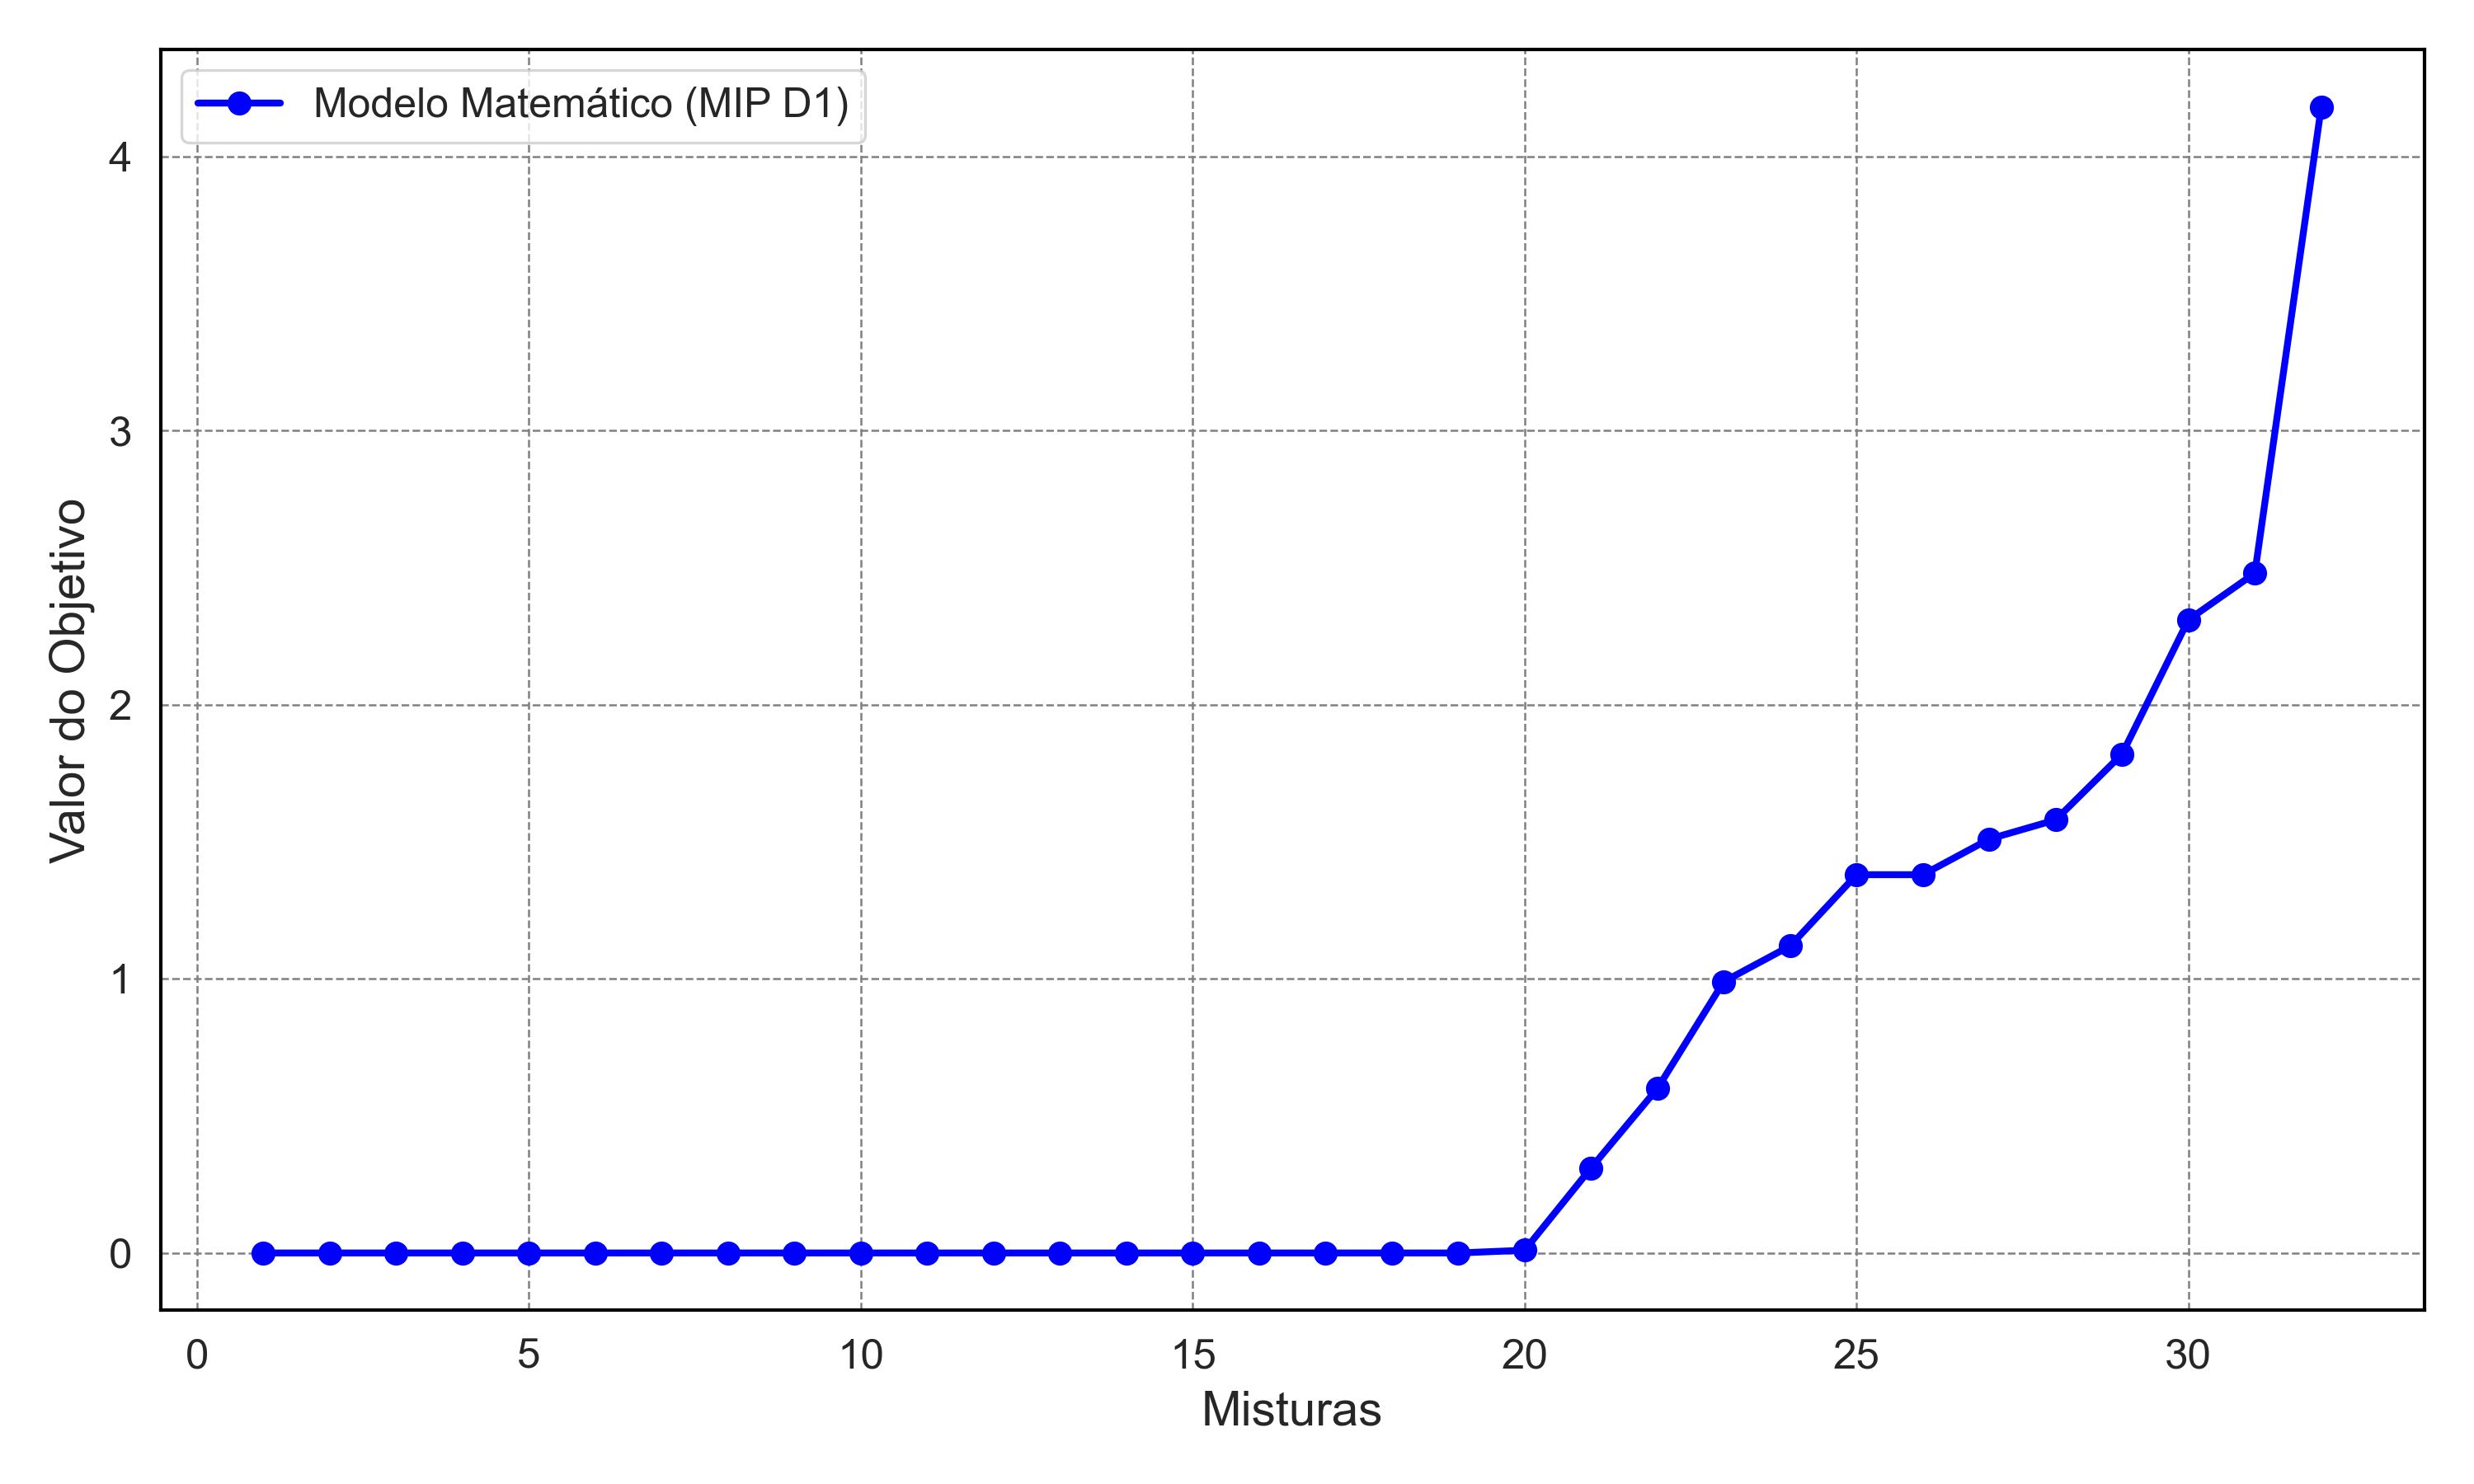
\includegraphics[width=1\textwidth]{figures/ModeloMatematicoQk1D1.png}
\end{figure}

O tempo computacional, especialmente no caso do modelo matemático, é pouco afetado pelas discretizações. A soma dos objetivos e sua variação ao longo das misturas são representados na Tabela \ref{tab:discretizacao_divergencia} e na Figura \ref{figure:DiscMM}, respectivamente.

\begin{table}[htp]
    \centering
    \caption{Impacto da discretização na soma do objetivo e divergência percentual, com 32 misturas.}
    \begin{tabular}{c c c}
         Discretização (D) & Soma Obj. & Divergência (\%) \\
         \hline
         \(1\)   & 19,67  & - \\
         \(2\)   & 19,96  & +1,47\% \\
         \(3\)   & 17,98  & -8,59\% \\
         \(5\)   & 16,92  & -13,98\% \\
         \(6\)   & 16,63  & -15,46\% \\
         \hline
    \end{tabular}
    \label{tab:discretizacao_divergencia}
\end{table}

\begin{figure}[hbt]
\centering
  \caption{Impacto das discretizações ao longo das misturas no modelo matemático.}   
  \label{figure:DiscMM}
  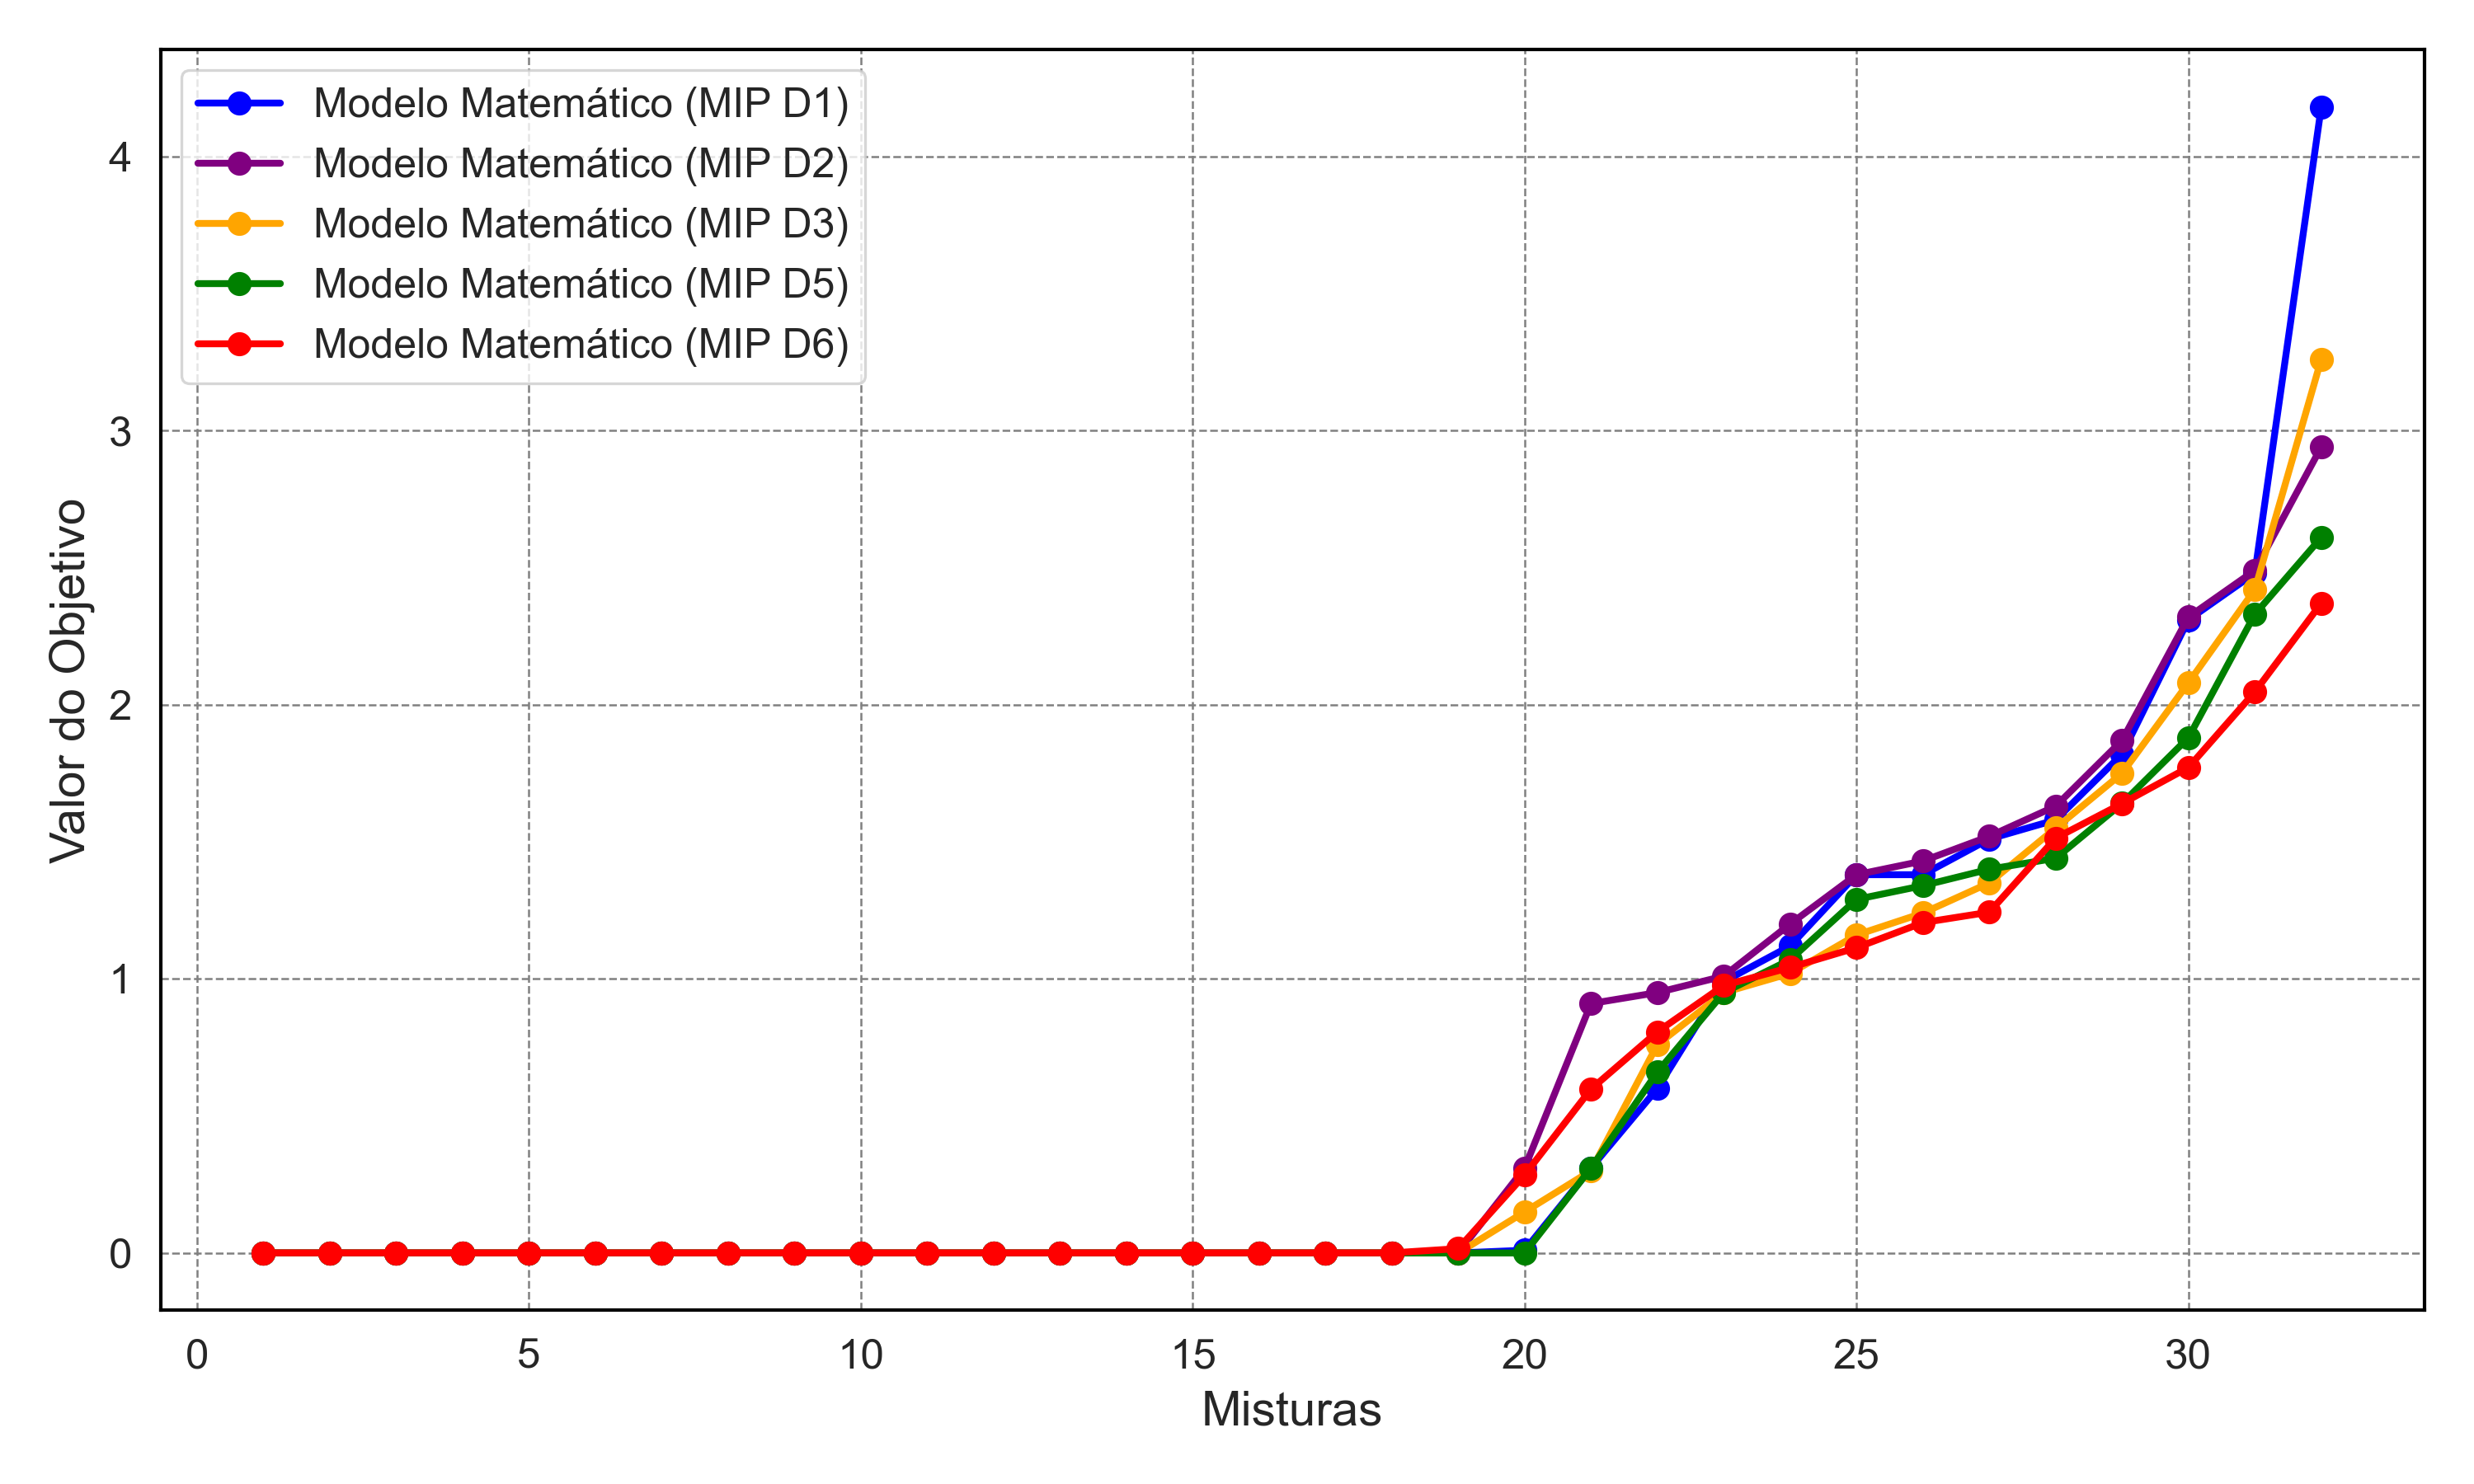
\includegraphics[width=1\textwidth]{figures/Discretizacao_comparacao.png}
\end{figure}

Como o AR e o modelo matemático são comparados sob as mesmas premissas de discretização, as posteriores análises são válidas e viabilizam os testes computacionais, porém divergem da situação real.

\section{APRENDIZADO POR REFORÇO}

A fim de tornar a solução viável computacionalmente e escolher o melhor modelo para a aplicação final no Gêmeo Digital Autônomo, uma série de testes e comparações foram feitos, entre diferentes discretizações, modelos de simulação e funções de recompensa.

\subsection{ABORDAGEM ESTÁTICA E DETERMINÍSTICA}

A Tabela \ref{tab:discretizacao} apresenta o impacto das diferentes discretizações propostas no tempo necessário para processar os 18.432.000 de \textit{timesteps} (iterações do modelo de simulação) definidos.

\begin{table}[htp]
    \centering
    \caption{Impacto da discretização no tempo computacional.}
    \begin{tabular}{c c}
    \toprule
    Discretização (D) & Tempo (horas) \\
    \midrule
    \(1\) & 646,71 \\
    \(2\) & 345,23 \\
    \(3\) & 156,11 \\
    \(5\) & 97,62  \\
    \(6\) & 62,49  \\
    \bottomrule
    \end{tabular}
    \label{tab:discretizacao}
\end{table}

Os resultados mostram que o esforço computacional diminui significativamente com o aumento da discretização (\(D\)), à medida que o problema se simplifica. A discretização \(D=6\) foi escolhida como padrão para os experimentos, pois apresentou um tempo computacional aceitável e não comprometeu a qualidade das soluções encontradas, como visto na Figura \ref{figure:DiscMM} e reafirmado pela Figura \ref{figure:DiscD1D6RLI}.

\begin{figure}[hbt]
\centering
  \caption{Comparação entre os modelos matemáticos (MIP D1), (MIP D6) e modelo de AR (RL I).} 
  \label{figure:DiscD1D6RLI}
  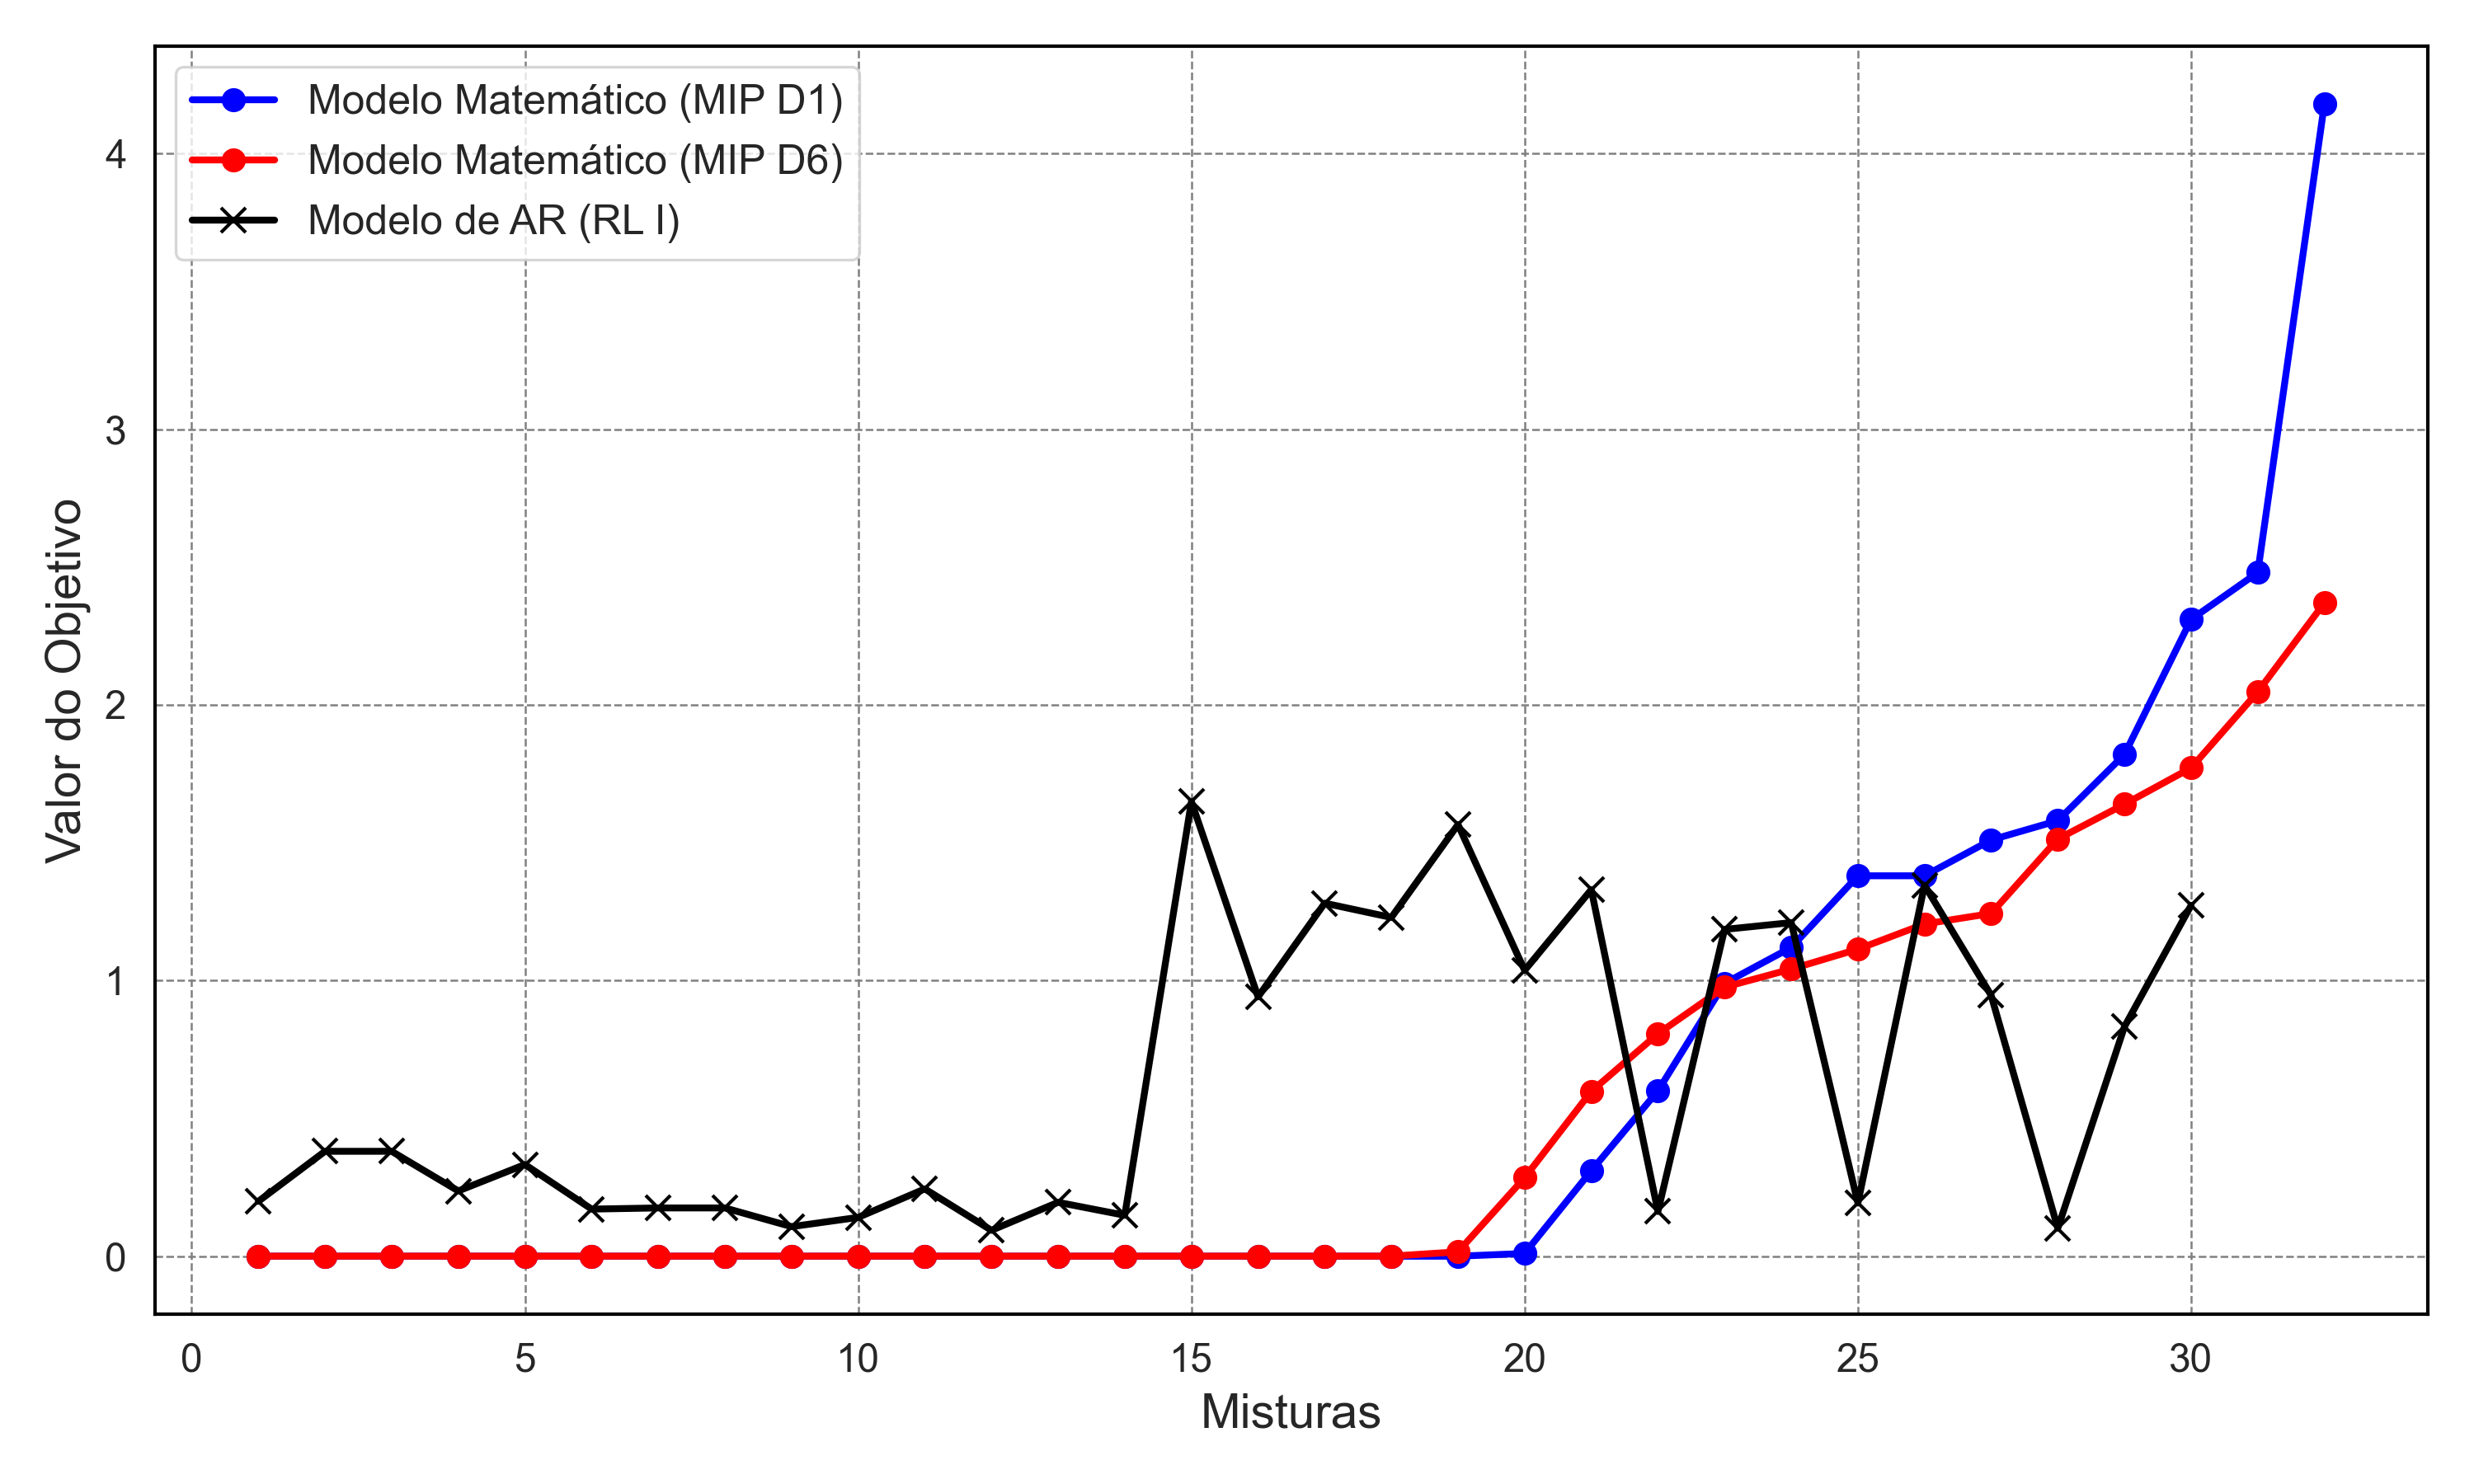
\includegraphics[width=1\textwidth]{figures/MIPD1D6RL1.png}
\end{figure}

No ambiente estático e sem aleatoriedade, os modelos de AR, que são inexatos na tratativa do problema, convergiram a um mesmo conjunto de soluções, após o treinamento, para todos os testes.

A fim de encontrar a melhor função de recompensa, dentre aquelas propostas, para implementar no modelo dinâmico, testes foram feitos sob as mesmas condições de tempo de treino: 18.432.000 \textit{timesteps}.

\begin{table}[htp]
    \centering
    \caption{Comparação entre os modelos quanto ao número de misturas factíveis, soma dos objetivos e \textit{Gap} de otimalidade.}
    \begin{tabular}{l c c c}
    \toprule
    Modelo & Mist. Factíveis & Soma dos Objetivos & \textit{Gap} \\
    \midrule
    MIP (D6)        & 33 & 19,67  & -       \\
    RL I            & 30 & 19,26  & 57,7\%  \\
    RL II           & 29 & 13,88  & 32,9\%  \\
    RL III (0.1)    & 30 & 18,53  & 51,7\%  \\
    RL III (0.2)    & 30 & 15,38  & 25,9\%  \\
    RL III (0.5)    & 30 & 16,18  & 32,4\%  \\
    RL III (1.0)    & 26 & 15,10  & 149,7\% \\
    RL IV           & 29 & 15,48  & 48,2\%  \\
    RL V            & 26 & 17,83  & 194,8\% \\
    RL VI           & 31 & 17,33  & 21,5\%  \\
    RL VII          & 30 & 14,29  & 17,0\%  \\
    \bottomrule
    \end{tabular}
    \label{tab:comparacao_rl}
\end{table}

Como dito anteriormente, no modelo matemático, as restrições são explicitamente impostas e qualquer solução infactível é descartada, garantindo, assim, mistura factível e performance próxima do ótimo global. Já no Aprendizado por Reforço (RL), as restrições são convertidas em recompensas e punições, o que, embora traga flexibilidade, pode levar a explotação local caso as penalizações não sejam bem calibradas, ou caso o tempo de treinamento não seja suficiente, resultando em buscas por recompensas imediatas e menor consistência de soluções.

Os resultados da Tabela \ref{tab:comparacao_rl} indicam que o modelo matemático atingiu o melhor desempenho como referência. O RL I, com penalização fixa, apresentou um \textit{gap} elevado devido à falta de flexibilidade na adaptação às restrições. O RL II, ao incorporar penalizações proporcionais e considerar o estoque, melhorou o equilíbrio entre qualidade e factibilidade, embora a adaptação tenha ocorrido de forma gradual. No RL III, o ajuste da penalização e do \textit{cliprange} trouxe um melhor equilíbrio, mas valores excessivos comprometeram a estabilidade da política. O RL IV, com histórico de decisões, não trouxe ganhos significativos, sugerindo que a inclusão de dados temporais não foi suficiente para melhorar o desempenho. Já o RL V, com penalização extrema, comprometeu severamente o aprendizado, resultando em baixa factibilidade e alto \textit{gap}.

Os modelos RL VI e RL VII apresentaram os melhores desempenhos. O RL VI, com incentivo adicional para soluções ótimas, obteve 31 misturas e reduziu o \textit{gap} para 21,5\%, sugerindo que recompensas positivas melhoram a convergência para soluções de alta qualidade. Já o RL VII, utilizando observação binária do estoque, alcançou 30 misturas e o menor \textit{gap} de 17,0\%, indicando que uma representação simplificada do ambiente contribui para um aprendizado mais eficiente e robusto.

O modelo matemático resolve as misturas encontrando soluções ótimas para a mistura instantânea, sem considerar períodos futuros. Em contrapartida, o AR aprimora o conjunto das misturas ao longo do tempo, maximizando a soma das recompensas. Conforme observado a partir da Mistura 23 na Figura \ref{figure:ModeloMatematicoRLVII}, o modelo matemático seleciona os melhores fardos para o momento presente, sem antecipar as necessidades futuras. Isso resulta na acumulação de fardos cujas características, em média, desviam significativamente do alvo ao longo do tempo. Já no modelo RL VII, com o AR, essa situação é atenuada, pois a diferença entre as propriedades das misturas e o alvo se mantém mais equilibrada ao longo do tempo.

\begin{figure}[hbt]
\centering
  \caption{Comparação entre modelo matemático (MIP D6) e modelo de AR (RL VII).}
  \label{figure:ModeloMatematicoRLVII}
  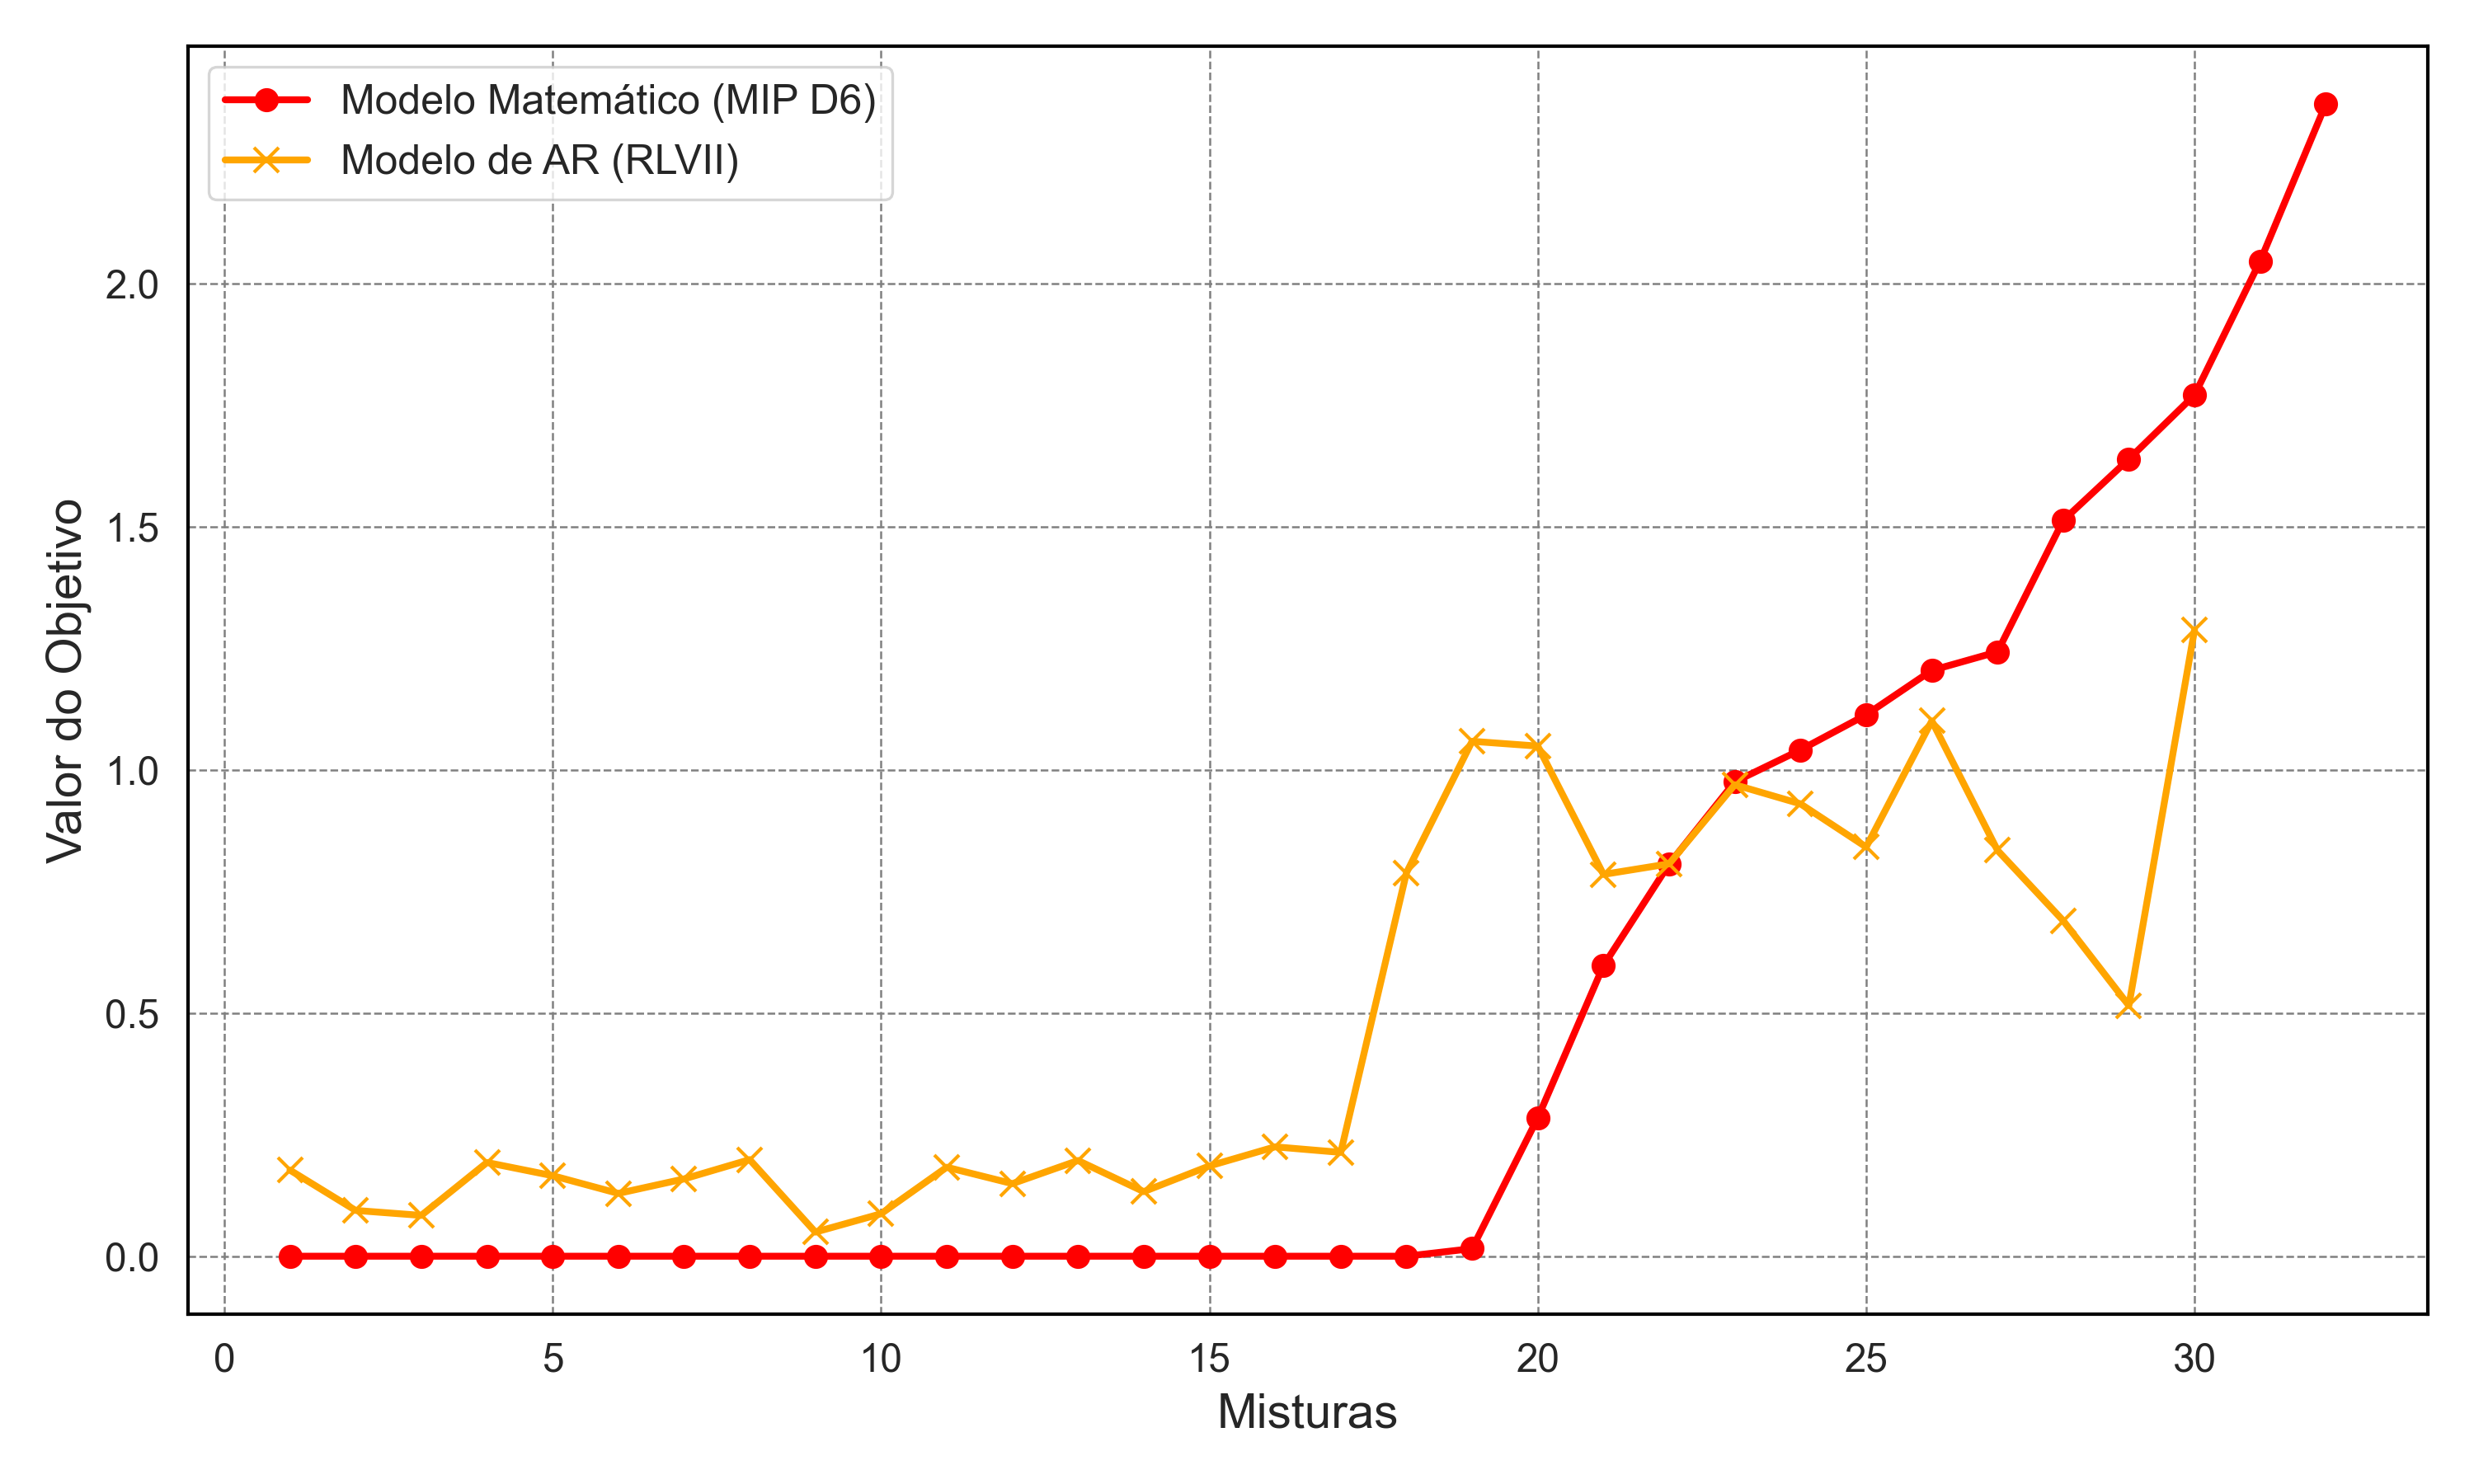
\includegraphics[width=1\textwidth]{figures/ModeloMatematicoRLVII.png}
\end{figure}

\subsection{ABORDAGEM DINÂMICA E ESTOCÁSTICA}

A Figura \ref{figure:DINRLVII} explicita que o modelo dinâmico de aprendizado por reforço (RL VII DIN) apresenta um desempenho mais consistente ao longo do tempo, resultando em menores variações nos valores do objetivo e uma melhor aderência aos parâmetros desejados. Como foram definidas múltiplas réplicas para o modelo dinâmico, a média dos valores do objetivo foi representada. Esse comportamento pode ser explicado pelo fato de o modelo considerar continuamente a chegada de novos fardos, ajustando as decisões com base nas condições futuras.

Em contraste, o modelo estático (RL VII), que opera com um estoque fixo e não se renova, tende a apresentar um aumento progressivo dos desvios das propriedades da mistura em relação ao alvo. À medida que os fardos mais adequados são utilizados, restam opções com características menos favoráveis, resultando em uma degradação gradual da qualidade das misturas.

A abordagem dinâmica permite uma gestão mais eficiente dos recursos ao distribuir de forma equilibrada os fardos ao longo do horizonte de planejamento. Isso se reflete em uma menor dispersão nos valores do objetivo e uma menor ocorrência de picos abruptos de erro, como evidenciado na comparação gráfica. Já o modelo estático, por não incorporar novas informações, apresenta uma variabilidade maior e um desempenho que se deteriora conforme o estoque disponível se reduz.

Como foram definidas múltiplas réplicas para o modelo dinâmico, a média dos valores do objetivo foi representada graficamente ao longo das misturas.

\begin{figure}[hbt]
\centering
  \caption{Comparação entre modelo de AR (RL VII) e modelo de AR dinâmico (RL VII DIN).}
  \label{figure:DINRLVII}
  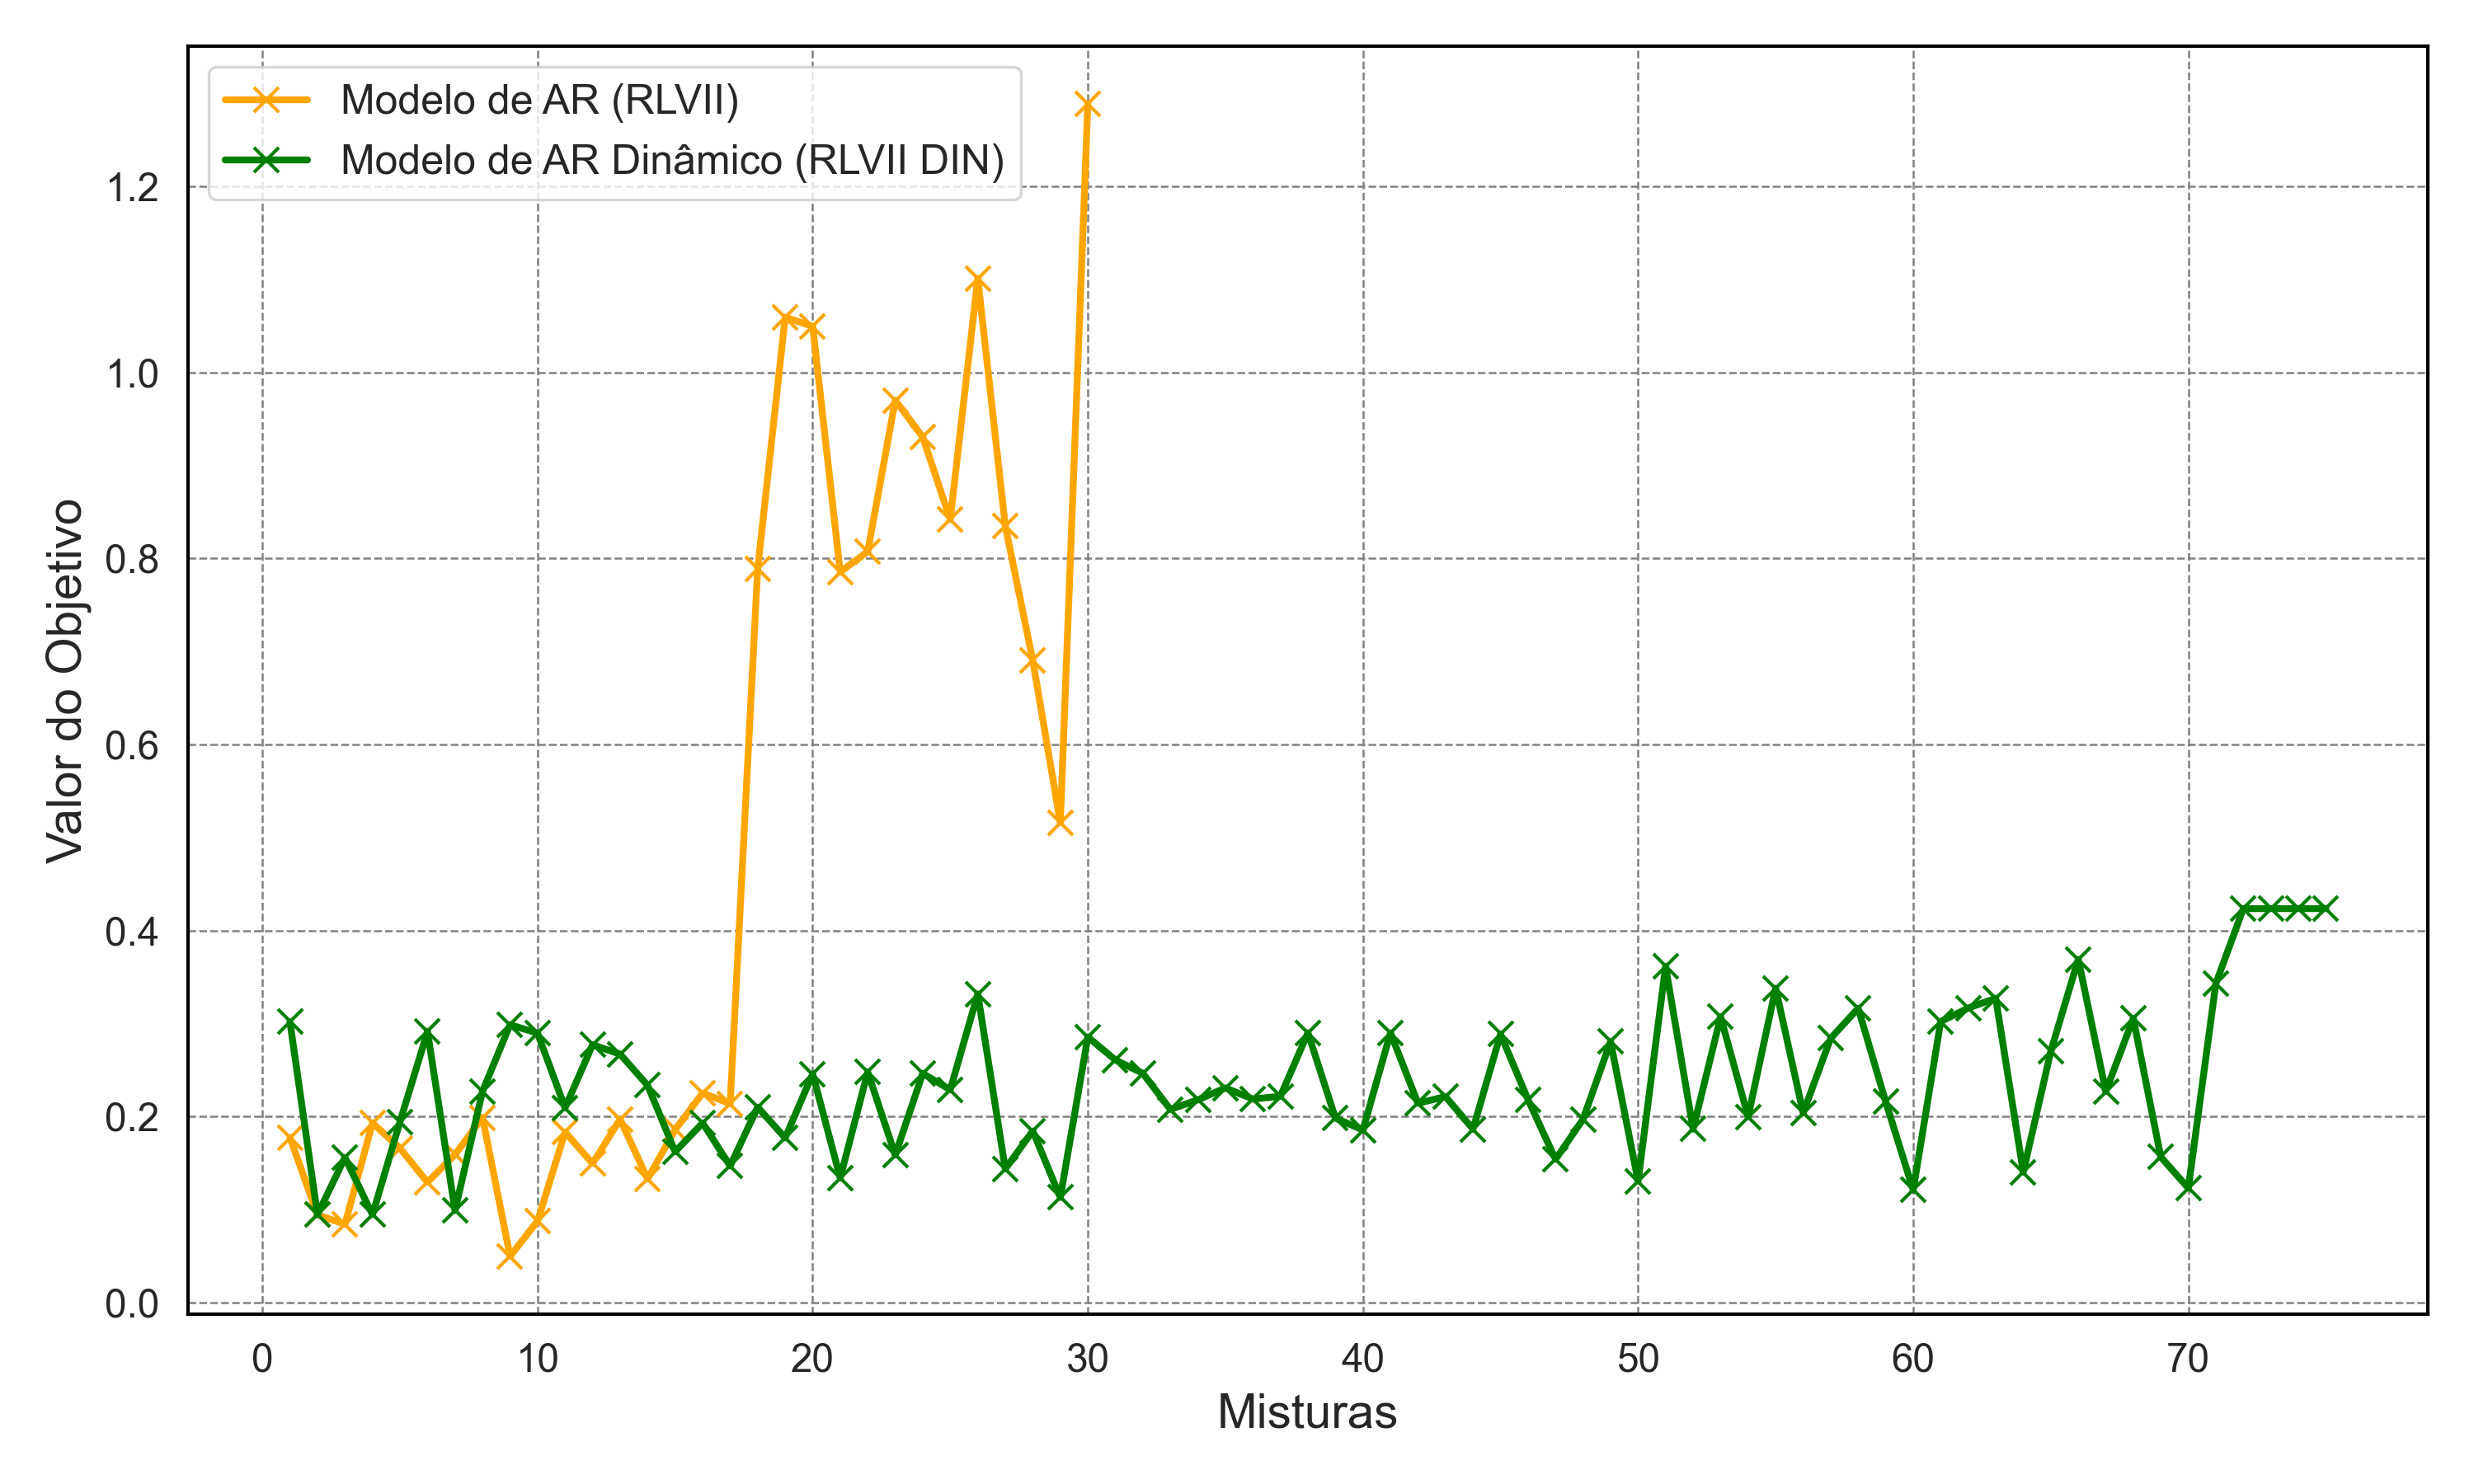
\includegraphics[width=1\textwidth]{figures/DINRLVII.png}
\end{figure}

\subsubsection{ANÁLISE ESTATÍSTICA DO MODELO DINÂMICO (RL VII DIN)}

Devido à incorporação de variabilidades inerentes ao processo real, no modelo de simulação, as soluções propostas não convergem para uma mesma escolha de fardos em todas as réplicas, como acontecera no modelo estático. Essa dispersão nos resultados mostra a importância de se quantificar a precisão estatística das réplicas, permitindo avaliar a robustez das estimativas obtidas, como a média e os intervalos de confiança.

Foram previamente definidas 10 misturas e, para cada réplica, o valor do objetivo médio de cada mistura foi calculado. Em seguida, os dados foram agregados por réplica (calculando-se a média dos valores de objetivo médio para cada grupo).

Os resultados obtidos são resumidos na Tabela~\ref{tab:resultados}.

\begin{table}[ht]
\centering
\caption{Métricas estatísticas agregadas por réplica}
\label{tab:resultados}
\begin{tabular}{@{}ll@{}}
\toprule
Métrica & Valor \\ \midrule
Número de réplicas (grupos únicos) & 10 \\
Média dos \emph{Objetivo Médio} por réplica & 0.2265 \\
Desvio padrão (S) & 0.0080 \\
Variância amostral (S\textsuperscript{2}) & 0.0001 \\ \midrule
Valor crítico \(Z\) (95\% de confiança) & 1.9600 \\
Número mínimo de réplicas (com \(E=0.5\)) & 0.00 (arredondado para 1) \\ \midrule
\(t\) crítico (df = 9) & 2.2622 \\
Margem de erro (usando \(t\)) & 0.0057 \\
Intervalo de confiança para a média & (0.2207, 0.2322) \\ \midrule
Quantil qui-quadrado \(1-\alpha/2\) (df = 9) & 19.0228 \\
Quantil qui-quadrado \(\alpha/2\) (df = 9) & 2.7004 \\
Intervalo de confiança para a variância & (0.0000, 0.0002) \\
\bottomrule
\end{tabular}
\end{table}

Observa-se que os 10 grupos de réplicas resultaram em uma média de 0.2265 para o objetivo médio, com um desvio padrão de 0.0080, indicando baixa variabilidade entre os grupos. A aplicação da fórmula para o número mínimo de réplicas, dada a margem de erro \(E = 0.5\), resultou em um valor inferior a 1 (arredondado para 1), evidenciando que o conjunto de 10 réplicas utilizado excede amplamente a quantidade mínima necessária para obter uma estimativa precisa da média.

O intervalo de confiança para a média, calculado com a distribuição \(t\) de \textit{Student}, foi estimado como \((0.2207, 0.2322)\), enquanto o intervalo de confiança para a variância, com base na distribuição qui-quadrado, foi determinado como \((0.0000, 0.0002)\).

Na Figura \ref{figure:replicas}, a variação do objetivo ao longo das misturas pode ser observada ao longo das 10 réplicas:

\begin{figure}[hbt]
\centering
  \caption{Réplicas (RL VII DIN).}
  \label{figure:replicas}
  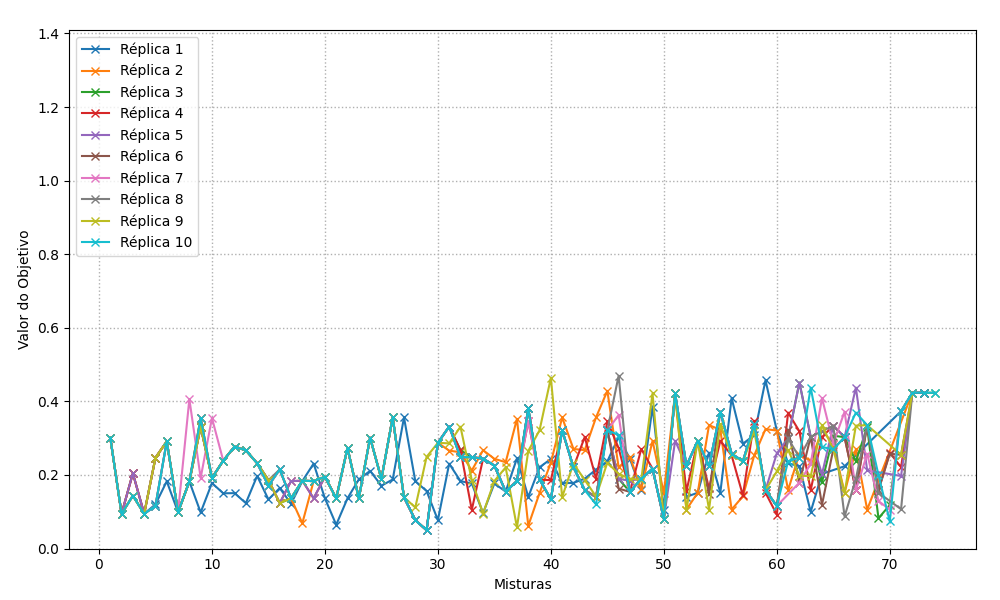
\includegraphics[width=1\textwidth]{figures/replicas.png}
\end{figure}

Na Tabela~\ref{tab:testes} são apresentados os resultados dos testes estatísticos realizados. Cada réplica contém os valores de objetivo para diversas misturas. Para cada réplica foram calculadas a média dos valores, que serviram de insumo para os testes a seguir.

\begin{table}[htp]
    \centering
    \caption{Resultados dos Testes Estatísticos}
    \label{tab:testes}
    \begin{tabular}{lcc}
    \toprule
    Teste & Estatística & p-valor \\
    \midrule
    Shapiro–Wilk     & 0.8201  & 0.0254 \\
    Levene           & 0.2992  & 0.9750 \\
    ANOVA (one-way)  & 0.5176  & 0.8624 \\
    Kruskal–Wallis   & 6.7732  & 0.6607 \\
    Pearson          & 0.3114  & 0.0000 \\
    Regressão Linear & \(\beta = 0.0014\), \(r = 0.3114\) & 0.0000 \\
    \bottomrule
    \end{tabular}
\end{table}

O teste de Shapiro–Wilk apresentou um p-valor de 0.0254, indicando a rejeição da hipótese de normalidade das médias das réplicas ao nível de 5\%. Em contrapartida, o teste de Levene obteve um p-valor de 0.9750, confirmando a homogeneidade das variâncias entre as réplicas, o que valida o uso de testes paramétricos, mesmo que os dados não sejam normalmente distribuídos. Tanto a ANOVA quanto o teste de Kruskal–Wallis não detectaram diferenças significativas entre as réplicas (p-valores de 0.8624 e 0.6607, respectivamente), demonstrando a consistência dos resultados do modelo. A análise de correlação de Pearson revelou uma correlação positiva moderada (r = 0.3114, p < 0.0001) entre o ID da mistura e o valor do objetivo, tendência esta confirmada pela regressão linear, que apontou uma inclinação de 0.0014, indicando que conforme as misturas são feitas e a incerteza propagada para as misturas à frente, o valor do objetivo aumenta gradativamente.

\subsection{PARÂMETROS DE TREINAMENTO}

A Figura \ref{fig:Recompensa} apresenta a evolução da recompensa nos modelos estático e dinâmico. No modelo estático (Figura \ref{fig:RecompensaESTATICO}), observa-se um crescimento gradual e previsível da recompensa, com oscilações reduzidas e estabilização rápida. Esse comportamento evidencia a capacidade do agente de aprender eficientemente em um ambiente sem incertezas, convergindo para uma característica mais explotatória de aprendizado.

No modelo dinâmico (Figura \ref{fig:RecompensaDINAMICO}), a recompensa cresce menos rapidamente, demorando mais para chegar na política ótima local, acompanhada por oscilações significativas na tentativa de encontrar uma melhor. Esse padrão reflete a necessidade de constante adaptação do agente diante das incertezas do ambiente, exigindo certo balanço entre exploração e explotação para lidar com a variabilidade das chegadas e propriedades dos itens.

\begin{figure}[hbt]
\centering
\caption{Recompensas no treinamento do AR.}
\label{fig:Recompensa}
\begin{subfigure}{0.48\textwidth}
    \centering
    \caption{Modelo Estático.}
    \label{fig:RecompensaESTATICO}
    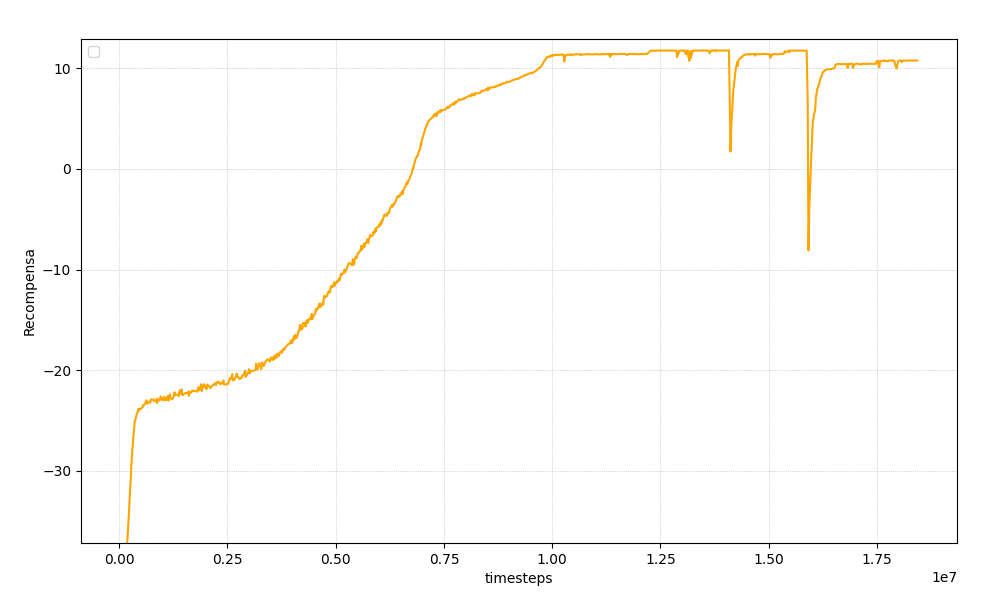
\includegraphics[width=1\textwidth]{figures/RecompensaESTATICO.png}
\end{subfigure}
\hfill
\begin{subfigure}{0.48\textwidth}
    \centering
    \caption{Modelo Dinâmico.}
    \label{fig:RecompensaDINAMICO}
    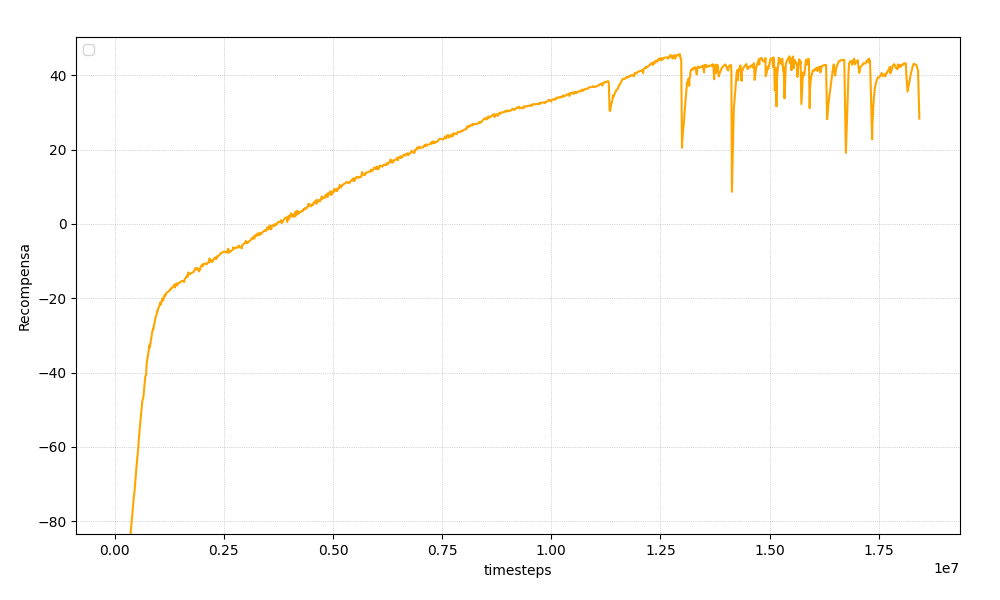
\includegraphics[width=1\textwidth]{figures/RecompensaDIN.png}
\end{subfigure}
\end{figure}

A Figura \ref{fig:ClipFraction} apresenta a evolução do parâmetro \textit{clip\_fraction} durante o treinamento nos modelos estático e dinâmico. Esse parâmetro representa a fração de atualizações de política que foram limitadas pelo hiperparâmetro de \textit{clipping}, influenciando diretamente a estabilidade do aprendizado, de forma que um valor maior de \textit{clip\_fraction} indica uma maior divergência entre políticas naquele instante.

No modelo estático (Figura \ref{fig:ClipFractionESTATICO}), observa-se uma queda acentuada do valor do \textit{clip\_fraction} no início do treinamento, seguida de oscilações esporádicas em estágios posteriores. Isso indica que, impulsionado pela previsibilidade do ambiente, as políticas são mais próximas entre si, conforme o treinamento ocorre.

No modelo dinâmico (Figura \ref{fig:ClipFractionDINAMICO}), o \textit{clip\_fraction} apresenta uma redução mais gradual, com oscilações intensas e frequentes após alcançar valores mínimos. Essa tendência indica que o agente tem maior dificuldade em encontrar estabilidade entre as políticas, quando comparada com a anterior.

\begin{figure}[hbt]
\centering
\caption{\textit{clip\_fraction} no treinamento do AR.}
\label{fig:ClipFraction}
\begin{subfigure}{0.48\textwidth}
    \centering
    \caption{Modelo Estático.}
    \label{fig:ClipFractionESTATICO}
    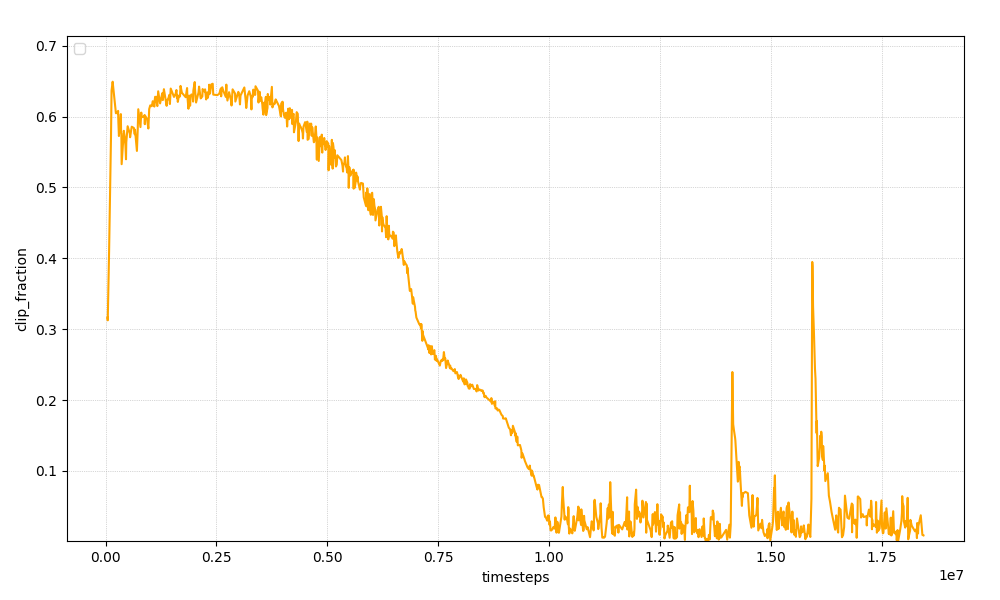
\includegraphics[width=1\textwidth]{figures/ClipFractionESTATICO.png}
\end{subfigure}
\hfill
\begin{subfigure}{0.48\textwidth}
    \centering
    \caption{Modelo Dinâmico.}
    \label{fig:ClipFractionDINAMICO}
    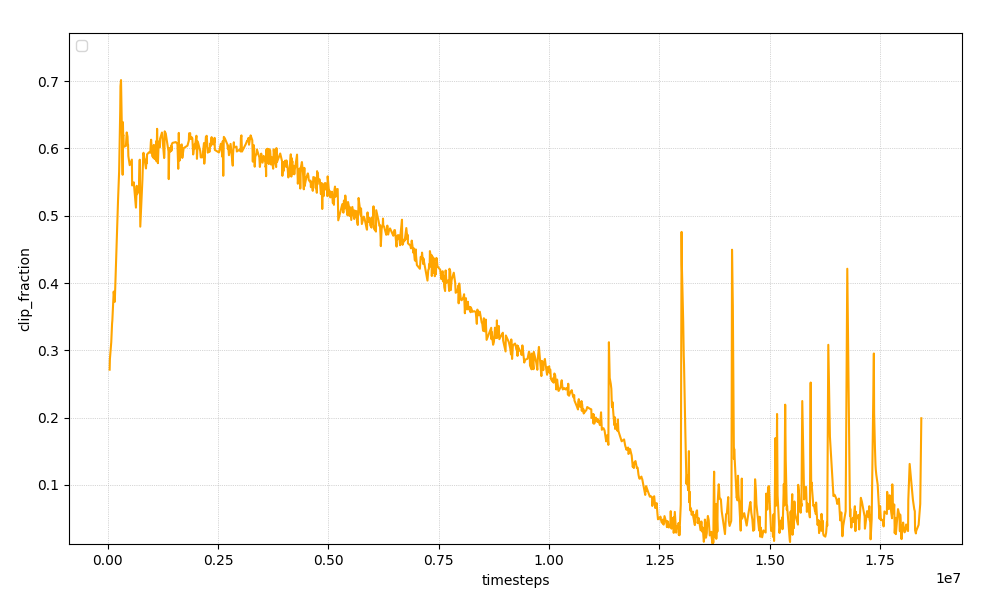
\includegraphics[width=1\textwidth]{figures/ClipFractionDIN.png}
\end{subfigure}
\end{figure}

A Figura \ref{fig:AproxKL} apresenta a evolução da divergência KL aproximada durante o treinamento nos modelos estático e dinâmico. Esse parâmetro avalia a proximidade entre distribuições de probabilidade das políticas sucessivas, refletindo a magnitude das mudanças na estratégia do agente.

No modelo estático (Figura \ref{fig:AproxKLESTATICO}), a divergência KL aumenta no início do treinamento, estabiliza-se e depois apresenta uma redução gradual. Isso sugere que as atualizações de política se tornam progressivamente menores conforme o agente converge para uma solução.

No modelo dinâmico (Figura \ref{fig:AproxKLDINAMICO}), a divergência KL permanece em níveis mais elevados por mais tempo e exibe picos frequentes. Isso indica que o agente realiza ajustes mais frequentes devido às mudanças constantes no ambiente.

\begin{figure}[hbt]
\centering
\caption{Divergência KL no treinamento do AR.}
\label{fig:AproxKL}
\begin{subfigure}{0.48\textwidth}
    \centering
    \caption{Modelo Estático.}
    \label{fig:AproxKLESTATICO}
    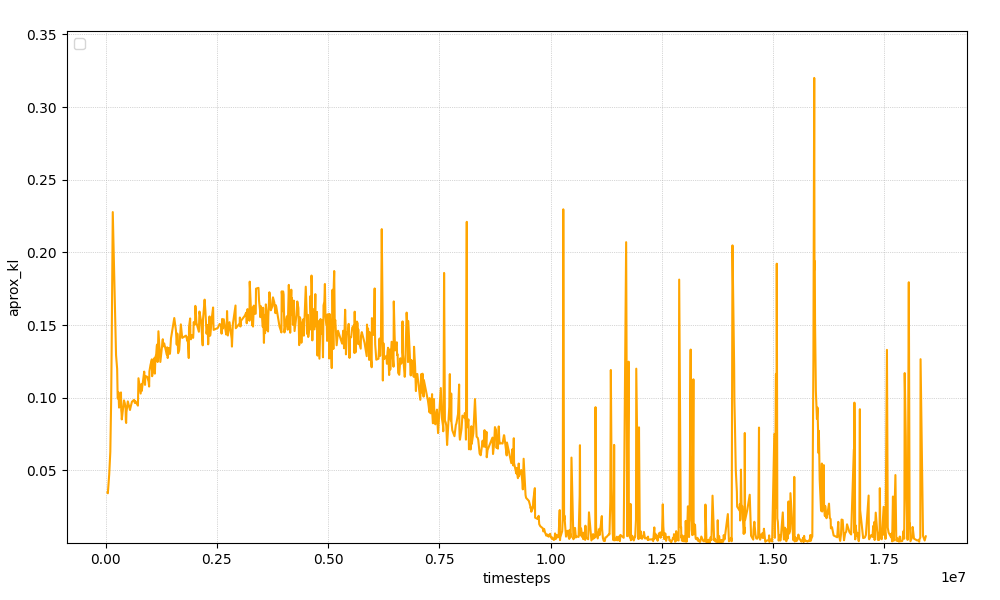
\includegraphics[width=1\textwidth]{figures/AproxKLESTATICO.png}
\end{subfigure}
\hfill
\begin{subfigure}{0.48\textwidth}
    \centering
    \caption{Modelo Dinâmico.}
    \label{fig:AproxKLDINAMICO}
    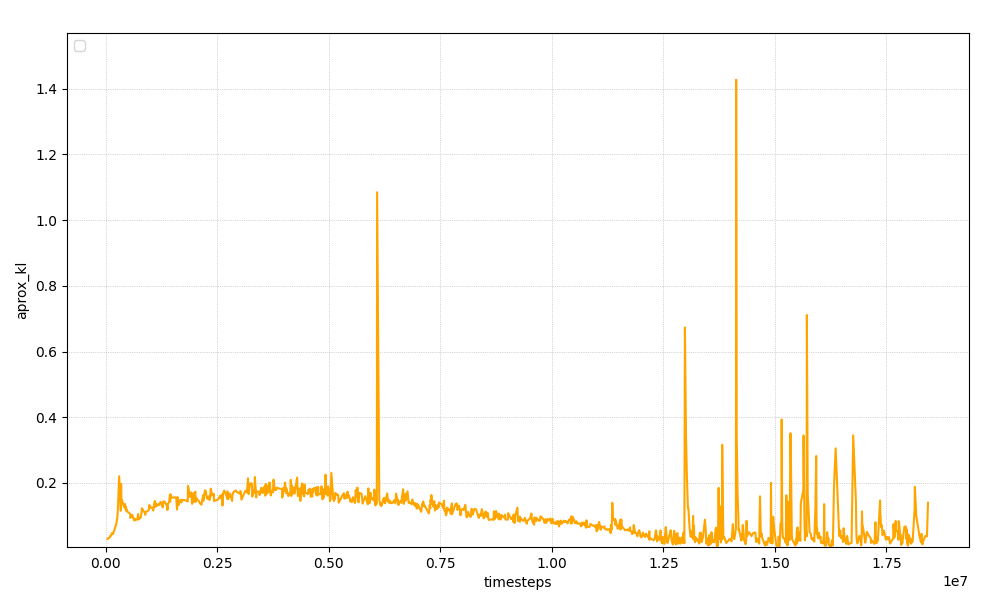
\includegraphics[width=1\textwidth]{figures/AproxKLDINAMICO.png}
\end{subfigure}
\end{figure}

\chapter{CONCLUSÃO}

O trabalho propõe um método alternativo para a mistura de algodão na fiação têxtil, avançando na implementação do Gêmeo Digital Autônomo por meio de ferramentas analíticas e de conectividade. O protocolo desenvolvido integra dados reais e modelos de Aprendizado por Reforço, permitindo uma abordagem adaptativa diante da variabilidade do algodão e das condições operacionais do processo produtivo. Diferente dos métodos tradicionais que oferecem soluções determinísticas e estáticas, o AR possibilita ajustes contínuos conforme novas informações se tornam disponíveis.

Ao atingir o nível 5 de maturidade do Gêmeo Digital, a solução proposta automatiza o processo ao conectar ferramentas complementares. A integração entre dados operacionais e o modelo de AR garante a replicação das dinâmicas do sistema, caracterizando a Dimensão Comportamental do Gêmeo Digital. Já a Dimensão Física é representada de forma simplificada, proporcionando rastreabilidade e controle das operações. Essa estrutura possibilita atualizações contínuas das decisões, operando tanto a montante, ao considerar as características dos fardos disponíveis, quanto a jusante, ao garantir que as misturas atendam às exigências da produção.

A validação do protocolo envolveu a análise de diferentes configurações do modelo de simulação, funções de recompensa e observações, resultando em uma abordagem que equilibra restrições operacionais e eficiência na resolução das misturas. Nos testes realizados, o AR apresentou um \textit{gap} de otimalidade de 17\% (em experimentos pareados ao modelo matemático) que, mesmo demonstrando viabilidade no planejamento das misturas, melhores resultados poderiam ter sido encontrados, caso mais poder computacional estivesse disponível. A aplicação em um cenário dinâmico evidenciou a capacidade do AR em ajustar a tomada de decisão progressivamente diante da chegada de novos fardos, mesmo sem informações exatas sobre suas propriedades e procedências. 

A conectividade estabelecida pelo Sistema de Informações Gerenciais, aliada ao Banco de Dados Relacional e à transmissão eficiente de dados, amplia a aplicabilidade do protocolo em ambientes reais. Novos fardos registrados no sistema atualizam automaticamente o Banco de Dados, refletindo mudanças no modelo de simulação. O agente de AR ajusta a alocação dos fardos e antecipa decisões conforme as expectativas futuras de estoque. Após definir a mistura, os dados são transmitidos via protocolo \textit{MODBUS} ao Sistema de Informações Gerenciais, permitindo que a solução seja visualizada e implementada na operação.

Esse fluxo contínuo, conectando o ambiente físico e virtual, consolida um protocolo de Gêmeo Digital Autônomo de ponta a ponta.













% ----------------------------------------------------------
% Referências bibliográficas
% ----------------------------------------------------------
\bibliography{bibliografia}





% ----------------------------------------------------------
% Glossário
% ----------------------------------------------------------
%
% Consulte o manual da classe abntex2 para orientações sobre o glossário.
%
%\glossary

% ----------------------------------------------------------
% Apêndices
% ----------------------------------------------------------

% ---
% Inicia os apêndices
% ---
\begin{apendicesenv}

% Imprime uma página indicando o início dos apêndices
%\partapendices

% ----------------------------------------------------------
% Apêndice A
% ----------------------------------------------------------
\chapter{DADOS E \textit{SCRIPTS}}

\begin{longtable}{c c c c c}
\caption{Estoque inicial e características médias por procedência.} \label{tab:estoque_inicial} \\
\hline
Procedência & Estoque Inicial & rd & \(+b\) & Micronaire \\
\hline
\endfirsthead
\multicolumn{5}{c}{\tablename\ \thetable\ -- Estoque inicial e características médias por procedência} \\
\hline
Procedência & Estoque Inicial & rd & \(+b\) & Micronaire \\
\hline
\endhead
\hline \multicolumn{5}{r}{} \\
\endfoot
\hline
\endlastfoot
1  & 151,00 & 73,00 & 8,50  & 4,64 \\ 
2  & 143,00 & 81,10 & 6,90  & 3,52 \\ 
3  & 10,00  & 74,40 & 8,20  & 4,28 \\ 
4  & 32,00  & 73,50 & 11,80 & 3,78 \\ 
5  & 132,00 & 64,40 & 13,30 & 3,73 \\ 
6  & 147,00 & 71,80 & 11,10 & 3,82 \\ 
7  & 104,00 & 75,30 & 9,30  & 3,99 \\ 
8  & 108,00 & 78,60 & 8,10  & 4,09 \\ 
9  & 119,00 & 73,70 & 10,10 & 3,07 \\ 
10 & 27,00  & 74,90 & 11,10 & 4,58 \\ 
11 & 44,00  & 79,30 & 7,20  & 3,88 \\ 
12 & 105,00 & 74,80 & 10,60 & 4,31 \\ 
13 & 132,00 & 63,00 & 9,70  & 3,59 \\ 
14 & 9,00   & 75,10 & 9,90  & 4,21 \\ 
15 & 95,00  & 72,90 & 10,80 & 4,02 \\ 
16 & 125,00 & 73,30 & 10,60 & 3,20 \\ 
17 & 140,00 & 73,70 & 9,60  & 4,16 \\ 
18 & 20,00  & 70,70 & 10,10 & 4,77 \\ 
19 & 21,00  & 71,70 & 10,10 & 4,71 \\ 
20 & 21,00  & 67,40 & 12,60 & 4,13 \\ 
21 & 21,00  & 72,50 & 10,50 & 4,78 \\ 
22 & 22,00  & 74,90 & 12,30 & 3,81 \\ 
23 & 118,00 & 74,30 & 10,60 & 3,71 \\ 
24 & 123,00 & 73,00 & 10,80 & 4,03 \\ 
25 & 85,00  & 76,90 & 7,80  & 3,89 \\ 
26 & 98,00  & 76,90 & 10,20 & 3,85 \\ 
27 & 22,00  & 75,10 & 11,30 & 4,16 \\ 
28 & 112,00 & 74,40 & 11,30 & 4,07 \\ 
29 & 3,00   & 76,00 & 9,00  & 3,94 \\ 
30 & 74,00  & 71,90 & 10,10 & 4,36 \\ 
31 & 62,00  & 76,20 & 6,30  & 3,91 \\ 
32 & 109,00 & 66,70 & 9,20  & 3,15 \\ 
33 & 0,00   & 74,30 & 9,50  & 0,00 \\ 
34 & 64,00  & 72,20 & 11,50 & 3,93 \\ 
35 & 4,00   & 77,30 & 9,00  & 4,11 \\ 
36 & 132,00 & 71,10 & 8,50  & 3,49 \\ 
37 & 1,00   & 75,60 & 9,70  & 3,48 \\ 
38 & 105,00 & 74,90 & 9,00  & 3,89 \\ 
39 & 126,00 & 76,80 & 10,60 & 3,78 \\ 
40 & 132,00 & 73,80 & 10,00 & 4,28 \\ 
41 & 1,00   & 74,60 & 10,60 & 3,69 \\ 
42 & 106,00 & 74,60 & 9,40  & 3,59 \\ 
43 & 45,00  & 75,00 & 9,00  & 3,95 \\ 
44 & 124,00 & 74,80 & 10,40 & 4,41 \\ 
45 & 69,00  & 74,70 & 10,30 & 4,11 \\ 
46 & 115,00 & 71,10 & 10,60 & 3,98 \\ 
47 & 78,00  & 73,10 & 9,50  & 3,90 \\ 
48 & 111,00 & 77,90 & 9,40  & 3,30 \\ 
49 & 46,00  & 72,70 & 12,50 & 3,83 \\ 
50 & 46,00  & 74,90 & 12,30 & 3,81 \\ 
51 & 132,00 & 82,80 & 8,10  & 3,75 \\ 
52 & 126,00 & 76,30 & 10,50 & 3,58 \\ 
53 & 110,00 & 67,80 & 7,10  & 4,36 \\ 
54 & 182,00 & 76,10 & 10,70 & 3,80 \\ 
55 & 48,00  & 73,80 & 10,30 & 3,94 \\ 
56 & 124,00 & 74,00 & 9,20  & 4,32 \\ 
57 & 93,00  & 76,50 & 11,30 & 3,86 \\ 
58 & 3,00   & 75,10 & 10,40 & 3,82 \\ 
59 & 76,00  & 72,40 & 9,90  & 3,84 \\ 
60 & 116,00 & 68,40 & 10,70 & 3,80 \\ 
\end{longtable}

\textit{Scripts}, arquivos e demais dados relevantes estão disponíveis no repositório do \textit{GitHub}: \href{https://github.com/FelipePCapalbo/TCC}{https://github.com/FelipePCapalbo/TCC}.


\end{apendicesenv}
% ---

%---------------------------------------------------------------------
% INDICE REMISSIVO
%---------------------------------------------------------------------
\phantompart
\printindex
%---------------------------------------------------------------------

\end{document}
